% This is the Reed College LaTeX thesis template. Most of the work
% for the document class was done by Sam Noble (SN), as well as this
% template. Later comments etc. by Ben Salzberg (BTS). Additional
% restructuring and APA support by Jess Youngberg (JY).
% Your comments and suggestions are more than welcome; please email
% them to cus@reed.edu
%
% See https://www.reed.edu/cis/help/LaTeX/index.html for help. There are a
% great bunch of help pages there, with notes on
% getting started, bibtex, etc. Go there and read it if you're not
% already familiar with LaTeX.
%
% Any line that starts with a percent symbol is a comment.
% They won't show up in the document, and are useful for notes
% to yourself and explaining commands.
% Commenting also removes a line from the document;
% very handy for troubleshooting problems. -BTS

% As far as I know, this follows the requirements laid out in
% the 2002-2003 Senior Handbook. Ask a librarian to check the
% document before binding. -SN

%%
%% Preamble
%%
% \documentclass{<something>} must begin each LaTeX document
%% twoside es útil para la impresión de libros
% \documentclass[12pt,twoside]{templates/unerthesis} 
\documentclass[12pt,oneside]{templates/unerthesis}

% Packages are extensions to the basic LaTeX functions. Whatever you
% want to typeset, there is probably a package out there for it.
% Chemistry (chemtex), screenplcays, you name it.
% Check out CTAN to see: https://www.ctan.org/
%%
%\ifxetex
%  \usepackage{polyglossia}
%  \setmainlanguage{spanish}
  % Tabla en lugar de cuadro
%  \gappto\captionsspanish{\renewcommand{\tablename}{Tabla}
%          \renewcommand{\listtablename}{Índice de tablas}}
%\else
%  \usepackage[spanish,es-tabla]{babel}
%\fi
%\usepackage[spanish]{babel}
%\usepackage[spanish,provide=*]{babel}


%\ifxetex
%  \usepackage{polyglossia}
%  \setmainlanguage{spanish}
  % Tabla en lugar de cuadro
%  \gappto\captionsspanish{\renewcommand{\tablename}{Tabla}
%          \renewcommand{\listtablename}{Índice de tablas}}
%\else
\usepackage[spanish,provide=*]{babel}
\addto\captionsspanish{
  \renewcommand{\tablename}{Tabla}
  \renewcommand{\listtablename}{Índice de tablas}
}
%\fi

\usepackage{graphicx,latexsym}
\usepackage{amsmath}
\usepackage{amssymb,amsthm}
\usepackage{longtable,booktabs,setspace}
\usepackage{chemarr} %% Useful for one reaction arrow, useless if you're not a chem major
\usepackage[hyphens]{url}
% Added by CII
%\usepackage{hyperref}
\usepackage[colorlinks = true,
            linkcolor = blue,
            urlcolor  = blue,
            citecolor = blue,
            anchorcolor = blue]{hyperref}
\usepackage{lmodern}
\usepackage{float}
\floatplacement{figure}{H}
% End of CII addition
\usepackage{rotating}
\usepackage{placeins} % para fijar la posición de las tablas con \FloatBarrier
\usepackage{calc}

\usepackage[]{natbib}

% Next line commented out by CII
%\usepackage{biblatex}
%\usepackage{natbib}
% Comment out the natbib line above and uncomment the following two lines to use the new
% biblatex-chicago style, for Chicago A. Also make some changes at the end where the
% bibliography is included.
%\usepackage{biblatex-chicago}
%\bibliography{thesis}


% Added by CII (Thanks, Hadley!)
% Use ref for internal links
\renewcommand{\hyperref}[2][???]{\autoref{#1}}
\def\chapterautorefname{Chapter}
\def\sectionautorefname{Section}
\def\subsectionautorefname{Subsection}
% End of CII addition

% Added by CII
\usepackage{caption}
\captionsetup{width=5in}
% End of CII addition

% \usepackage{times} % other fonts are available like times, bookman, charter, palatino

% Syntax highlighting #22

% To pass between YAML and LaTeX the dollar signs are added by CII
\title{Herramienta de simulación para dar soporte a la enseñanza de arquitectura de computadoras}
\author{Ruiz Jose Maria}
% The month and year that you submit your FINAL draft TO THE LIBRARY (May or December)
\date{2025}
\division{}
\advisor{Director: Colombani Marcelo Alberto}
\institution{Universidad de Nacional de Entre Rios}
\degree{Maestría en Sistemas de Información}
%If you have two advisors for some reason, you can use the following
% Uncommented out by CII
% End of CII addition

%%% Remember to use the correct department!
\department{}
% if you're writing a thesis in an interdisciplinary major,
% uncomment the line below and change the text as appropriate.
% check the Senior Handbook if unsure.
%\thedivisionof{The Established Interdisciplinary Committee for}
% if you want the approval page to say "Approved for the Committee",
% uncomment the next line
%\approvedforthe{Committee}

% Added by CII
%%% Copied from knitr
%% maxwidth is the original width if it's less than linewidth
%% otherwise use linewidth (to make sure the graphics do not exceed the margin)
\makeatletter
\def\maxwidth{ %
  \ifdim\Gin@nat@width>\linewidth
    \linewidth
  \else
    \Gin@nat@width
  \fi
}
\makeatother

% Definir los comandos CSLLeftMargin y CSLRightInline
\newcommand{\CSLLeftMargin}[1]{#1} % Define \CSLLeftMargin como un simple contenedor
\newcommand{\CSLRightInline}[1]{#1} % Define \CSLRightInline como un simple contenedor


%Added by @MyKo101, code provided by @GerbrichFerdinands
\newlength{\cslhangindent}
\setlength{\cslhangindent}{1.5em}
\newenvironment{CSLReferences}[2] % #1: hanging indent, #2: entry spacing
 {\setlength{\parindent}{0pt}%
  \setlength{\leftskip}{#1 pt\relax}% % Agregar unidad `pt`
  \setlength{\parskip}{#2 pt\relax}% % Agregar unidad `pt`
  \everypar{\setlength{\hangindent}{\cslhangindent}}}
 {\par}

\setlength\parindent{0pt}

% Added by CII

\providecommand{\tightlist}{%
  \setlength{\itemsep}{0pt}\setlength{\parskip}{0pt}}

\Acknowledgements{

}

\Dedication{

}

\Preface{

}

\Abstract{

}

	% Paquetes adicionales
\usepackage{listings}
\usepackage{xcolor}
\usepackage[utf8]{inputenc}
\usepackage[T1]{fontenc}

\lstdefinelanguage{nasm}{
  morekeywords={section, global, extern, mov, add, sub, mul, div, inc, dec, push, pop, call, ret, jmp, je, jne, jz, jnz, loop, int},
  sensitive=false,
  morecomment=[l];,
  morestring=[b]",
}

\lstset{literate=%
    {á}{{\'a}}1
    {é}{{\'e}}1
    {í}{{\'i}}1
    {ó}{{\'o}}1
    {ú}{{\'u}}1
    {Á}{{\'A}}1
    {É}{{\'E}}1
    {Í}{{\'I}}1
    {Ó}{{\'O}}1
    {Ú}{{\'U}}1
    {ñ}{{\~n}}1
    {Ñ}{{\~N}}1
}

\lstset{
  basicstyle=\ttfamily\small,
  breaklines=true,
  frame=single,
  language=nasm,
  keywordstyle=\color{blue},
  commentstyle=\color{gray},
  stringstyle=\color{red},
  showstringspaces=false,
  numbers=left,
  numberstyle=\tiny\color{gray},
  stepnumber=1,
  numbersep=5pt,
  tabsize=2,
  captionpos=b,
  breakatwhitespace=false,
  showspaces=false,
  showtabs=false,
  columns=flexible,
  keepspaces=true,
}
	\usepackage{booktabs}
\usepackage{longtable}
\usepackage{array}
\usepackage{multirow}
\usepackage{wrapfig}
\usepackage{float}
\usepackage{colortbl}
\usepackage{pdflscape}
\usepackage{tabu}
\usepackage{threeparttable}
\usepackage{threeparttablex}
\usepackage[normalem]{ulem}
\usepackage{makecell}
\usepackage{xcolor}
% End of CII addition
%%
%% End Preamble
%%
%
\let\chaptername\relax
\begin{document}
%\bibliographystyle{apalike}
%\bibliographystyle{IEEEtran}

% Everything below added by CII
  \maketitle

\frontmatter % this stuff will be roman-numbered
\pagestyle{empty} % this removes page numbers from the frontmatter



%  \hypersetup{linkcolor=black}
  \setcounter{tocdepth}{1}
  \setlength{\parskip}{0pt}
  \tableofcontents

\setlength\parskip{1em plus 0.1em minus 0.2em}

  \listoftables

  \listoffigures



\mainmatter % here the regular arabic numbering starts
\pagestyle{fancyplain} % turns page numbering back on

\hypertarget{resumen}{%
\chapter*{Resumen}\label{resumen}}
\addcontentsline{toc}{chapter}{Resumen}

Existe un consenso creciente en el uso de herramientas de simulación en la enseñanza para procesos dinámicos complejos, como las operaciones intrínsecas de la computadora, que permiten representar de forma visual e interactiva la organización y arquitectura interna de la computadora, facilitando así la comprensión de su funcionamiento por parte de los alumnos y el desarrollo de los temas por parte del docente. En este contexto, los simuladores juegan una pieza clave en el campo de la Arquitectura de Computadoras, permitiendo conectar fundamentos teóricos con la experiencia práctica, simplificando abstracciones y haciendo más rica la labor docente.
La arquitectura x86 es ampliamente utilizada en computadoras de escritorio y servidores. Este documento pretende realizar una comparación de los simuladores x86 que más se adecuan en el dictado de la asignatura Arquitectura de Computadoras de la carrera Licenciatura en Sistemas, establecer los criterios de evaluación y evaluar los simuladores seleccionados de acuerdo con estos criterios.

La presente investigación surge en el marco del proyecto de investigación I/D novel PID-UNER 7065: ``Enseñanza/aprendizaje de asignatura Arquitectura de Computadoras con herramientas de simulación de sistemas de cómputos''. El Proyecto es llevado a cabo en la Facultad de Ciencias de la Administración de la Universidad Nacional de Entre Ríos, se vincula directamente con la asignatura Arquitectura en Computadoras que se dicta en segundo año de la carrera Licenciatura en Sistemas perteneciente a la Facultad de Ciencias de la Administración de la Universidad Nacional de Entre Ríos.

Palabras clave: x86, simulador, aprendizaje, enseñanza, arquitectura de computadoras.

\hypertarget{agradecimientos}{%
\chapter*{Agradecimientos}\label{agradecimientos}}
\addcontentsline{toc}{chapter}{Agradecimientos}

Agradecimientos aquí.

\hypertarget{intro}{%
\chapter{Introducción}\label{intro}}

El uso cotidiano de dispositivos como computadoras personales, teléfonos móviles y relojes inteligentes está sustentado en arquitecturas computacionales específicas, cuya comprensión es fundamental para el desarrollo eficiente de soluciones informáticas.

Es esencial que los estudiantes de Arquitectura de Computadoras comprendan tanto la estructura como el funcionamiento interno de una computadora, y adquieran experiencia práctica con ellas. Para lograrlo, es fundamental disponer de un laboratorio bien equipado con el hardware adecuado y suficiente tiempo para que los estudiantes se familiaricen con las herramientas prácticas. En este contexto, se han desarrollado numerosos simuladores que facilitan la comprensión de la estructura y el funcionamiento de las computadoras, proporcionando valiosas experiencias de aprendizaje. Este trabajo se inscribe en dicha problemática educativa y busca contribuir con el desarrollo de una herramienta de simulación adaptada a las necesidades de la enseñanza de arquitectura de computadoras.

Esta tesis, inscrita en la Maestría en Sistemas de Información de la Facultad de Ciencias de la Administración, está directamente vinculada con el proyecto de investigación I/D novel PID-UNER 7065, titulado ``Enseñanza/aprendizaje de Arquitectura de Computadoras con herramientas de simulación de sistemas de cómputo'', desarrollado en la Facultad de Ciencias de la Administración de la Universidad Nacional de Entre Ríos \protect\hyperlink{ref-colombani_pid_2022}{{[}1{]}}.

La asignatura Arquitectura de Computadoras forma parte del plan de estudios de la carrera de Licenciatura en Sistemas, Universidad Nacional de Entre Ríos. Su objetivo es que los estudiantes comprendan la estructura y funcionamiento de las computadoras, y la ejecución lógica de un programa a nivel de instrucciones de máquina.

Para comprender los fundamentos de la arquitectura de computadoras, resulta necesario abordar su estructura básica y funcionamiento interno, comenzando por una descripción funcional general del sistema.

Desde una perspectiva funcional, una computadora es un sistema que capta datos de entrada, los procesa de acuerdo con instrucciones codificadas, y produce salidas a través de dispositivos periféricos o almacenamiento. Esta dinámica operativa constituye la base para comprender su arquitectura interna y los principios que rigen su diseño.

El procesamiento se realiza a través del procesador o CPU, y es en este componente donde los estudiantes encuentran mayor complejidad y dificultades para comprender su funcionamiento.

A pesar de que es posible explicar las partes del procesador, su funcionamiento, la interacción de sus componentes y enseñar lenguaje ensamblador mediante prácticas, los estudiantes suelen tener dificultades para lograr una comprensión completa del funcionamiento.

Sin embargo, la utilización de simuladores permite afianzar los conocimientos de los temas vistos en las clases teóricas, por ello, los simuladores deben ser simples, intuitivos y visualmente atractivos, para que los estudiantes puedan centrarse en los conceptos de arquitectura y no en el aprendizaje de la herramienta en sí.

La simulación es un término de uso diario en muchos contextos: medicina, militar, entretenimiento, educación, etc., debido a que permite ayudar a comprender cómo funciona un sistema, responder preguntas como ``qué pasaría si'', con el fin de brindar hipótesis sobre cómo o por qué ocurren ciertos fenómenos.

En este contexto, es necesario comprender con mayor profundidad qué se entiende por simulación y cómo esta técnica puede aplicarse en entornos educativos, se define simulación como el proceso de imitar el funcionamiento de un sistema a medida que avanza en el tiempo. Para llevar a cabo una simulación, es necesario construir un modelo conceptual que represente las características y comportamientos del sistema de interés. La simulación permite observar cómo dicho modelo evoluciona en el tiempo, replicando dinámicas reales o hipotéticas \protect\hyperlink{ref-banks_discrete-event_2010}{{[}2{]}}, \protect\hyperlink{ref-law_simulation_2015}{{[}3{]}}, \protect\hyperlink{ref-robinson_simulation_2014}{{[}4{]}}.

Con los avances en el mundo digital, la simulación se ha convertido en una metodología de solución de problemas indispensable para ingenieros, docentes, diseñadores y gerentes. La complejidad intrínseca de los sistemas informáticos los hace difícil comprender y costosos de desarrollar sin utilizar simulación \protect\hyperlink{ref-law_simulation_2015}{{[}3{]}}.

Muchas veces en el ámbito educativo, resulta difícil transmitir fundamentos teóricos de la organización y arquitectura interna de las computadoras debido a la complejidad de los procesos involucrados. Cuando se emplean exclusivamente métodos de enseñanza tradicionales ---como pizarras, libros de texto o diapositivas---, estos resultan insuficientes para representar de manera efectiva las complejidades involucradas en la arquitectura de las computadoras \protect\hyperlink{ref-lion_simuladores_2005}{{[}5{]}}, \protect\hyperlink{ref-contreras_uso_2010}{{[}6{]}}, \protect\hyperlink{ref-garcia-garcia_pbbcache_2020}{{[}7{]}}.

Es evidente la necesidad de utilizar nuevas tecnologías como recursos didácticos y medios de transferencia de conocimiento, ya que ayudan a los estudiantes a relacionar conceptos abstractos con realidades concretas. Estas tecnologías permiten situar al estudiante en un contexto que imita aspectos de la realidad, posibilitando la detección y análisis de problemáticas semejantes a las que se presentan en entornos reales. Este enfoque promueve un mejor entendimiento a través del trabajo exploratorio, la inferencia, el aprendizaje por descubrimiento y el desarrollo de habilidades \protect\hyperlink{ref-nova_tool_2013}{{[}8{]}}, \protect\hyperlink{ref-mustafa_evaluating_2010}{{[}9{]}}.

Un simulador de arquitectura es una herramienta que imita el hardware de un sistema, representando sus aspectos arquitectónicos y funciones. Permiten realizar cambios, pruebas y ejecutar programas sin riesgo de dañar componentes ni depender de equipos físicos disponibles \protect\hyperlink{ref-radivojevic_design_2011}{{[}10{]}}.

Algunas herramientas ofrecen una representación en forma visual e interactiva de la organización y arquitectura interna de la computadora, facilitando así la comprensión de su funcionamiento. En este sentido, los simuladores juegan una pieza clave en el campo de la Arquitectura de Computadores, permitiendo conectar fundamentos teóricos con la experiencia práctica, simplificando abstracciones y facilitando la labor docente \protect\hyperlink{ref-nikolic_survey_2009}{{[}11{]}}, \protect\hyperlink{ref-hasan_survey_2012}{{[}12{]}}, \protect\hyperlink{ref-hennessy2017computer}{{[}13{]}}, \protect\hyperlink{ref-stallings_computer_2021}{{[}14{]}}.

Dentro del estudio de las arquitecturas de computadoras, la arquitectura x86 ocupa un lugar destacado debido a su amplia difusión y compatibilidad. A continuación, se presenta una breve evolución de esta arquitectura, que justifica su inclusión en el diseño de herramientas de simulación para la enseñanza. Comenzó con el procesador Intel 8086 en 1978 como una arquitectura de 16 bits. Evolucionó a una arquitectura de 32 bits con el procesador Intel 80386 en 1985 (i386 o x86-32) y posteriormente a 64 bits con las extensiones de AMD (AMD64) y su adopción por Intel (Intel 64) \protect\hyperlink{ref-intel_64_2025}{{[}15{]}}, \protect\hyperlink{ref-amd_developer_2024}{{[}16{]}}.

A pesar de la aparición de nuevas arquitecturas como ARM o RISC-V, que serán analizadas comparativamente en capítulos posteriores, la arquitectura x86 conserva una alta relevancia en contextos educativos y profesionales. Por ello, se considera pertinente su inclusión como base para el desarrollo de herramientas de simulación.

Un procesador x86-64 mantiene la compatibilidad con los modos x86 existentes de 16 y 32 bits, y permite ejecutar aplicaciones de 16 y 32 bits, como así también de 64 bits. Esta compatibilidad hacia atrás protege las principales inversiones en aplicaciones y sistemas operativos desarrollados para la arquitectura x86 \protect\hyperlink{ref-intel_64_2025}{{[}15{]}}, \protect\hyperlink{ref-amd_developer_2024}{{[}16{]}}, \protect\hyperlink{ref-abel_ibm_2000}{{[}17{]}}.

Por ello, la enseñanza de la arquitectura x86 es de gran relevancia en la asignatura Arquitecturas de Computadoras debido a los diferentes temas que aborda.

Como alternativa al equipamiento físico, los simuladores permiten suplir limitaciones de hardware y tiempo, brindando una experiencia de aprendizaje más accesible y replicable \protect\hyperlink{ref-skrien_cpu_2001}{{[}18{]}}.

\hypertarget{justificaciuxf3n}{%
\section{Justificación}\label{justificaciuxf3n}}

Los estudiantes y docentes de la asignatura de Arquitectura de Computadoras enfrentan múltiples desafíos a la hora de abordar los complejos conceptos teóricos inherentes a la arquitectura x86. Para los estudiantes, en particular, la introducción a la arquitectura de una computadora puede resultar abrumadora debido a la abstracción y el nivel de detalle técnico requerido. Por su parte, los docentes se ven limitados en la capacidad de ilustrar estos conceptos de manera gradual y progresiva debido a la falta de herramientas didácticas específicas para esta arquitectura. Ante estos desafíos, los simuladores juegan un papel crucial como herramientas de apoyo, al permitir la exploración y experimentación con los conceptos de forma visual e interactiva.

La necesidad de desarrollar un simulador específico para la arquitectura x86 se fundamenta en las limitaciones de los simuladores actuales, que no se adaptan de manera efectiva al plan de estudios específico de la asignatura Arquitectura de Computadoras, tal como se dicta en la Universidad Nacional de Entre Ríos. Aunque existen simuladores que apoyan la enseñanza de la arquitectura x86 en otros contextos \protect\hyperlink{ref-radivojevic_design_2011}{{[}10{]}}, \protect\hyperlink{ref-nikolic_survey_2009}{{[}11{]}}, estos tienden a incluir una gran cantidad de contenidos preestablecidos. Si bien dichos contenidos son relevantes, introducir la arquitectura x86 en su totalidad desde las primeras instancias del curso puede resultar contraproducente para estudiantes principiantes, debido a la complejidad técnica y a la extensa cantidad de conceptos involucrados.

Esta tesis propone un enfoque alternativo: el desarrollo de una herramienta de simulación específicamente diseñada para apoyar la enseñanza de los contenidos de la asignatura Arquitectura de Computadoras. El sistema simulará una computadora basada en la arquitectura x86, ofreciendo una representación progresiva de su estructura y funcionamiento. Abordará de forma modular los principales componentes del sistema: la unidad central de procesamiento (CPU), la memoria principal, el módulo de entrada/salida (E/S) y los buses de comunicación.

Entre sus funcionalidades clave, permitirá:
- Visualizar en detalle cada una de las etapas del ciclo de ejecución de instrucciones (fetch y execute).
- Trabajar con un repertorio limitado y escalable de instrucciones en lenguaje ensamblador.
- Ejecutar programas de forma paso a paso o completa.
- Gestionar interrupciones básicas para simular la interacción con periféricos como teclado y pantalla.
- Evaluar el rendimiento de los programas a partir de métricas observables durante la simulación.

Estas características facilitarán una comprensión progresiva de la arquitectura x86 y promoverán una experiencia de aprendizaje alineada con los objetivos del curso.

\begin{table}[!h]
\centering
\caption{\label{tab:funcionalidadessimulador}Funcionalidades principales del simulador propuesto}
\centering
\resizebox{\ifdim\width>\linewidth\linewidth\else\width\fi}{!}{
\begin{tabular}[t]{>{\raggedright\arraybackslash}p{4cm}|>{\raggedright\arraybackslash}p{5cm}>{\raggedright\arraybackslash}p{5cm}}
\toprule
\multicolumn{1}{>{\centering\arraybackslash}p{4cm}}{\cellcolor[HTML]{D3D3D3}{\textbf{Componente}}} & \multicolumn{1}{>{\centering\arraybackslash}p{5cm}}{\cellcolor[HTML]{D3D3D3}{\textbf{Funcionalidad.Principal}}} & \multicolumn{1}{>{\centering\arraybackslash}p{5cm}}{\cellcolor[HTML]{D3D3D3}{\textbf{Propósito.Didáctico}}}\\
\midrule
\textbf{CPU} & Ciclo de instrucción, ejecución paso a paso & Comprender la secuencia de ejecución\\
\textbf{Memoria} & Lectura/escritura en tiempo real & Visualizar acceso a datos\\
\textbf{E/S} & Gestión básica de teclado/pantalla & Simular interacción con periféricos\\
\textbf{Instrucciones} & Conjunto limitado y ampliable & Acompañar el avance del curso\\
\textbf{Evaluación} & Métricas de rendimiento & Analizar eficiencia de programas\\
\bottomrule
\end{tabular}}
\end{table}

Contar con un simulador adaptado específicamente a los contenidos de esta asignatura no solo facilita el proceso de aprendizaje, al presentar los conceptos de manera progresiva y alineada con la currícula, sino que también permite una experiencia de aprendizaje contextualizada. Esto fomenta un aprendizaje significativo, en el cual los estudiantes pueden conectar teoría y práctica de manera efectiva a través de una herramienta diseñada para abordar de forma gradual y específica los conceptos fundamentales del curso.

Para garantizar que el simulador sea robusto, modular, flexible y fácil de modificar o ampliar, se explorará la utilización de técnicas formales de modelado y simulación, como las redes de Petri y DEVS (Discrete Event System Specification). Estas técnicas permiten una separación conceptual entre las capas de modelado y simulación, lo cual facilita tanto la comprensión del software como su adaptación. Además, estas metodologías permiten que las simulaciones escalen de forma transparente, posibilitando su ejecución en entornos de cómputo paralelo o distribuido sin necesidad de modificar el modelo, lo que representa una ventaja significativa en términos de escalabilidad \protect\hyperlink{ref-peterson_petri_1981}{{[}19{]}}, \protect\hyperlink{ref-zeigler_theory_2000}{{[}20{]}}, \protect\hyperlink{ref-zeigler_theory_2018}{{[}21{]}}.

\hypertarget{objetivos}{%
\section{Objetivos}\label{objetivos}}

El objetivo principal de esta tesis es desarrollar una herramienta de simulación centrada en la arquitectura x86, orientada a fortalecer los procesos de enseñanza y aprendizaje de la asignatura Arquitectura de Computadoras. La herramienta estará alineada con los contenidos y objetivos formativos establecidos en la currícula vigente. En función de este objetivo general, se plantean los siguientes objetivos específicos:

\begin{enumerate}
\def\labelenumi{\arabic{enumi}.}
\tightlist
\item
  Estudiar y evaluar diferentes herramientas actuales de simulación destinadas a dar apoyo a la enseñanza de la arquitectura x86.
\item
  Diseñar e implementar una herramienta didáctica que facilite la enseñanza de los contenidos clave de la asignatura Arquitectura de Computadoras. Para ello, la herramienta deberá contemplar las siguientes funcionalidades:

  \begin{itemize}
  \tightlist
  \item
    Una visión global de la estructura y funcionamiento de la computadora.
  \item
    Generación y ejecución de programas en ensamblador.
  \item
    Repertorio de instrucciones x86 reducido y habilitado progresivamente.
  \item
    Simulación visual e interactiva de micropasos de instrucciones.
  \item
    Gestión de interrupciones y comunicación con periféricos.
  \item
    Medidas de rendimiento de ejecución de programas.
  \end{itemize}
\end{enumerate}

\hypertarget{metodologuxeda-de-desarrollo}{%
\section{Metodología de desarrollo}\label{metodologuxeda-de-desarrollo}}

La metodología de desarrollo de este simulador específico para la arquitectura x86 sigue una serie de etapas diseñadas para garantizar una progresión coherente y eficaz desde la fase de análisis hasta el diseño e implementación del simulador, de manera que se ajuste al plan de estudios de la asignatura Arquitectura de Computadoras en la Universidad Nacional de Entre Ríos.

\begin{enumerate}
\def\labelenumi{\arabic{enumi}.}
\item
  Análisis de requerimientos: En esta etapa inicial, se identifican y definen los objetivos específicos del simulador, así como los requerimientos técnicos y pedagógicos necesarios para su alineación con la currícula. Este análisis establece una base sólida y clara para todas las fases subsecuentes del proyecto, asegurando que el simulador cumpla con las necesidades educativas y técnicas del curso.
\item
  Revisión y recopilación de información: Se realiza una investigación sistemática sobre los simuladores existentes que abordan la arquitectura x86, considerando su aplicabilidad en contextos educativos. Este paso incluye un análisis de las características, ventajas y limitaciones de los simuladores existentes, proporcionando una comprensión más profunda del contexto educativo y permitiendo identificar áreas de mejora en relación con el objetivo del proyecto.
\item
  Estudio comparativo: A partir de la información recopilada, se realiza un estudio comparativo detallado de las características de los simuladores disponibles en el mercado. Esta etapa busca evaluar cuáles de sus funcionalidades pueden adaptarse o modificarse y cuáles deberían excluirse, de acuerdo con los objetivos del simulador y las necesidades específicas del plan de estudios. Los hallazgos de este análisis comparativo constituirán una base sólida para orientar las decisiones de diseño del simulador.
\item
  Diseño y planificación del simulador: Con base en los hallazgos previos, se define la arquitectura, las funcionalidades y los módulos específicos del simulador. El diseño se enfoca en facilitar el aprendizaje progresivo de los estudiantes, implementando un repertorio de instrucciones que se habiliten a medida que avanzan en el curso. En esta etapa, se utilizan técnicas formales de modelado, como redes de Petri y DEVS (Discrete Event System Specification), para establecer una estructura modular, robusta y flexible que facilite tanto la comprensión como la modificación futura de la herramienta.
\item
  Construcción y desarrollo: En esta fase, se lleva a cabo la implementación del simulador de acuerdo con el diseño previamente definido. Cada funcionalidad se implementa y verifica de manera secuencial, asegurando su conformidad con los requerimientos técnicos y pedagógicos definidos. También se realizan pruebas parciales para asegurar la precisión y funcionalidad de cada módulo, lo que permite identificar y corregir errores tempranamente.
\item
  \textbf{Evaluación y ajuste}: Finalmente, se somete el simulador a una serie de pruebas con estudiantes o expertos en la materia para evaluar su efectividad en el aprendizaje de los conceptos de arquitectura de computadoras. Los resultados obtenidos en esta fase permiten realizar ajustes y optimizaciones necesarias, mejorando la herramienta y asegurando que cumpla con su propósito educativo de manera efectiva.
\end{enumerate}

\hypertarget{organizaciuxf3n-del-documento}{%
\section{Organización del documento}\label{organizaciuxf3n-del-documento}}

El resto de este documento se estructura de la siguiente manera:

\begin{itemize}
\item
  En el Capítulo (\ref{arquitectura}), se presenta una descripción detallada de la arquitectura x86, definiendo sus características y el conjunto de instrucciones que la componen. Esta base teórica es fundamental para comprender los aspectos que se simularán en el proyecto.
\item
  El Capítulo (\ref{simulacion}) explora el papel de la simulación desde una perspectiva didáctica, enfatizando su valor como herramienta de apoyo en la enseñanza de Arquitectura de Computadoras. Aquí se revisan los beneficios de los simuladores en la enseñanza y los desafíos que ayudan a resolver en la formación de los estudiantes.
\item
  En el Capítulo (\ref{comparativa}), se realiza un análisis comparativo de los simuladores actuales, evaluándolos según criterios previamente establecidos. Este análisis permite identificar las limitaciones y fortalezas de cada simulador y establecer el contexto para la propuesta de esta tesis.
\item
  Finalmente, en el Capítulo (\ref{desarrollo}), se describe el desarrollo de un simulador específico que se ajusta a los objetivos de enseñanza y aprendizaje de la arquitectura x86 en el contexto de la currícula. Este simulador está diseñado como una herramienta práctica y accesible para facilitar la comprensión de conceptos complejos en la asignatura.
\end{itemize}

\hypertarget{arquitectura}{%
\chapter{Arquitectura de computadoras}\label{arquitectura}}

Este capítulo aborda los conceptos fundamentales de la arquitectura de computadoras, incluyendo las filosofías de diseño CISC y RISC, la evolución de la arquitectura x86 y una introducción al lenguaje ensamblador. Estos temas constituyen la base necesaria para comprender el funcionamiento interno de los sistemas informáticos.

\hypertarget{introducciuxf3n-a-la-arquitectura-de-computadoras}{%
\section{Introducción a la arquitectura de computadoras}\label{introducciuxf3n-a-la-arquitectura-de-computadoras}}

La arquitectura de computadoras es una disciplina central en el campo de la informática que estudia el diseño, la organización y la interacción entre los componentes de un sistema computacional. Esta área abarca tanto aspectos de hardware como de software que interactúan directamente con él, proporcionando principios fundamentales para construir sistemas eficientes, robustos y adaptables. Comprender su funcionamiento resulta esencial para analizar cómo se implementan, optimizan y escalan los sistemas informáticos en diversos contextos tecnológicos \protect\hyperlink{ref-stallings_computer_2021}{{[}14{]}}, \protect\hyperlink{ref-tanenbaum_structured_2016}{{[}22{]}}, \protect\hyperlink{ref-murdocca_principles_2000}{{[}23{]}}, \protect\hyperlink{ref-bryant2015computer}{{[}24{]}}.

Uno de los conceptos clave en esta disciplina es la distinción entre \textbf{arquitectura de computadoras} y \textbf{organización de computadoras}. La arquitectura se refiere a los elementos visibles para el programador, como el conjunto de instrucciones, los registros y los modos de direccionamiento. La organización, en cambio, se enfoca en los detalles físicos de implementación, tales como el diseño de circuitos y los ciclos de reloj necesarios para cada operación \protect\hyperlink{ref-hennessy2017computer}{{[}13{]}}, \protect\hyperlink{ref-stallings_computer_2021}{{[}14{]}}, \protect\hyperlink{ref-tanenbaum_structured_2016}{{[}22{]}}, \protect\hyperlink{ref-murdocca_principles_2000}{{[}23{]}}, \protect\hyperlink{ref-bryant2015computer}{{[}24{]}}.

Distinguir esta diferencia es crucial para analizar cómo los diseños arquitectónicos han evolucionado en respuesta a las crecientes demandas de rendimiento, eficiencia energética y escalabilidad. En este sentido, arquitecturas como ARM y RISC-V se han consolidado en sistemas embebidos y dispositivos móviles debido a su simplicidad estructural y bajo consumo energético \protect\hyperlink{ref-waterman_risc-v_2014}{{[}25{]}}, \protect\hyperlink{ref-harris2015digital}{{[}26{]}}, \protect\hyperlink{ref-null_essentials_2014}{{[}27{]}}. En contraste, la arquitectura x86 ha adoptado un enfoque híbrido que combina características de CISC y RISC, permitiéndole adaptarse a los exigentes requerimientos del mercado \protect\hyperlink{ref-stallings_computer_2021}{{[}14{]}}, \protect\hyperlink{ref-bryant2015computer}{{[}24{]}}, \protect\hyperlink{ref-patterson_computer_2014}{{[}28{]}}.

El análisis de una arquitectura de computadoras implica examinar múltiples dimensiones técnicas que inciden en su desempeño y aplicabilidad. Entre las más relevantes se encuentran:

\begin{itemize}
\tightlist
\item
  \textbf{Repertorio de instrucciones}: conjunto de operaciones que el procesador puede ejecutar directamente.
\item
  \textbf{Capacidad de procesamiento}: determinada por el número de bits con los que opera la CPU (por ejemplo, 32 o 64 bits).
\item
  \textbf{Modos de direccionamiento de memoria}: mecanismos mediante los cuales una instrucción accede a posiciones de memoria, como el direccionamiento directo, indirecto, segmentado o lineal.
\item
  \textbf{Jerarquía de memoria y mecanismos de entrada/salida}: estructuras que influyen en la eficiencia del acceso a datos y en la interacción con dispositivos periféricos.
\item
  \textbf{Grado de paralelismo}: capacidad de ejecutar múltiples instrucciones o tareas simultáneamente, ya sea a nivel de instrucción (ILP) o de procesos (TLP).
\end{itemize}

Estos dimensiones técnicas adquieren especial relevancia en sistemas contemporáneos aplicados a inteligencia artificial, internet de las cosas (IoT), computación en la nube y ciberseguridad, donde el equilibrio entre rendimiento, consumo energético y escalabilidad resulta determinante \protect\hyperlink{ref-harris2015digital}{{[}26{]}}, \protect\hyperlink{ref-patterson_computer_2016}{{[}29{]}}, \protect\hyperlink{ref-belli2020iot}{{[}30{]}}.

Un componente esencial en el estudio de esta disciplina es la \textbf{arquitectura del conjunto de instrucciones (ISA, por sus siglas en inglés)}, que define la interfaz entre el hardware y el software \protect\hyperlink{ref-hennessy2017computer}{{[}13{]}}. La ISA especifica las operaciones disponibles, la codificación de las instrucciones y las formas de manipular los datos. Esta interfaz es fundamental para el diseño de compiladores, sistemas operativos y herramientas de simulación, ya que permite abstraer el funcionamiento del hardware a nivel lógico y facilita la portabilidad del software.

El diseño arquitectónico implica tomar decisiones que suponen compromisos (\emph{trade-offs}), tales como la complejidad del hardware frente al rendimiento, o la eficiencia energética frente a la flexibilidad funcional. Estas decisiones determinan la aplicabilidad de una arquitectura en distintos dominios tecnológicos. Por ejemplo:

\begin{itemize}
\tightlist
\item
  La arquitectura \textbf{x86} resulta adecuada para entornos que requieren alto rendimiento y compatibilidad con software legado.
\item
  La arquitectura \textbf{ARM} se prefiere en dispositivos móviles debido a su bajo consumo energético \protect\hyperlink{ref-harris2015digital}{{[}26{]}}, \protect\hyperlink{ref-patterson_computer_2016}{{[}29{]}}, \protect\hyperlink{ref-belli2020iot}{{[}30{]}}.
\item
  \textbf{RISC-V}, por su parte, destaca por su apertura, modularidad y flexibilidad, lo que la convierte en una alternativa atractiva para investigación, docencia y aplicaciones personalizadas \protect\hyperlink{ref-waterman_risc-v_2014}{{[}25{]}}, \protect\hyperlink{ref-patterson_computer_2017}{{[}31{]}}.
\end{itemize}

En síntesis, el estudio de la arquitectura de computadoras permite comprender el funcionamiento interno de los sistemas, optimizar el desarrollo de soluciones tecnológicas complejas y fomentar la innovación en ingeniería de sistemas. Su enseñanza resulta fundamental en la formación en ciencias de la computación y disciplinas afines.

Desde una perspectiva educativa, el uso de herramientas de simulación contribuye a una comprensión progresiva de los conceptos arquitectónicos, al permitir experimentar con distintas arquitecturas y observar de forma interactiva el comportamiento del hardware \protect\hyperlink{ref-akram2019survey}{{[}32{]}}, \protect\hyperlink{ref-menchonherramientas}{{[}33{]}}. Esta dimensión didáctica adquiere especial importancia en el desarrollo de la herramienta propuesta en esta tesis, centrada en la arquitectura x86. Dicha arquitectura, ampliamente difundida en contextos académicos e industriales, también presenta desafíos significativos desde el punto de vista pedagógico, debido a su complejidad estructural y diversidad funcional.

\hypertarget{arquitecturas-von-neumann-y-harvard}{%
\section{Arquitecturas Von Neumann y Harvard}\label{arquitecturas-von-neumann-y-harvard}}

Comprender las arquitecturas modernas requiere el análisis de dos modelos conceptuales fundamentales que sentaron las bases del diseño actual de sistemas computacionales: Von Neumann y Harvard. Estos modelos arquitectónicos no solo constituyen la base teórica de muchas arquitecturas contemporáneas, sino que también permiten identificar sus fortalezas, limitaciones y áreas de aplicación.

\hypertarget{arquitectura-von-neumann}{%
\subsection{Arquitectura Von Neumann}\label{arquitectura-von-neumann}}

La arquitectura Von Neumann, formalizada por John von Neumann en 1945 en su influyente documento ``First Draft of a Report on the EDVAC'' \protect\hyperlink{ref-vonneumann1945first}{{[}34{]}}, establece un modelo computacional en el cual tanto los datos como las instrucciones residen en una única memoria y comparten un mismo bus de comunicación. Esta arquitectura se caracteriza por sus cuatro componentes fundamentales: la unidad central de procesamiento (CPU), la unidad de control, la memoria y los dispositivos de entrada/salida. La unificación del espacio de memoria facilita el diseño del sistema y la programación, sin embargo, esta unificación también origina una limitación conocida como el `cuello de botella de Von Neumann', que se refiere a la imposibilidad de acceder simultáneamente a datos e instrucciones debido al uso compartido del mismo bus, lo cual reduce la eficiencia del procesamiento, particularmente en aplicaciones con uso intensivo de datos \protect\hyperlink{ref-hennessy2017computer}{{[}13{]}}, \protect\hyperlink{ref-stallings_computer_2021}{{[}14{]}}.

\begin{figure}

{\centering 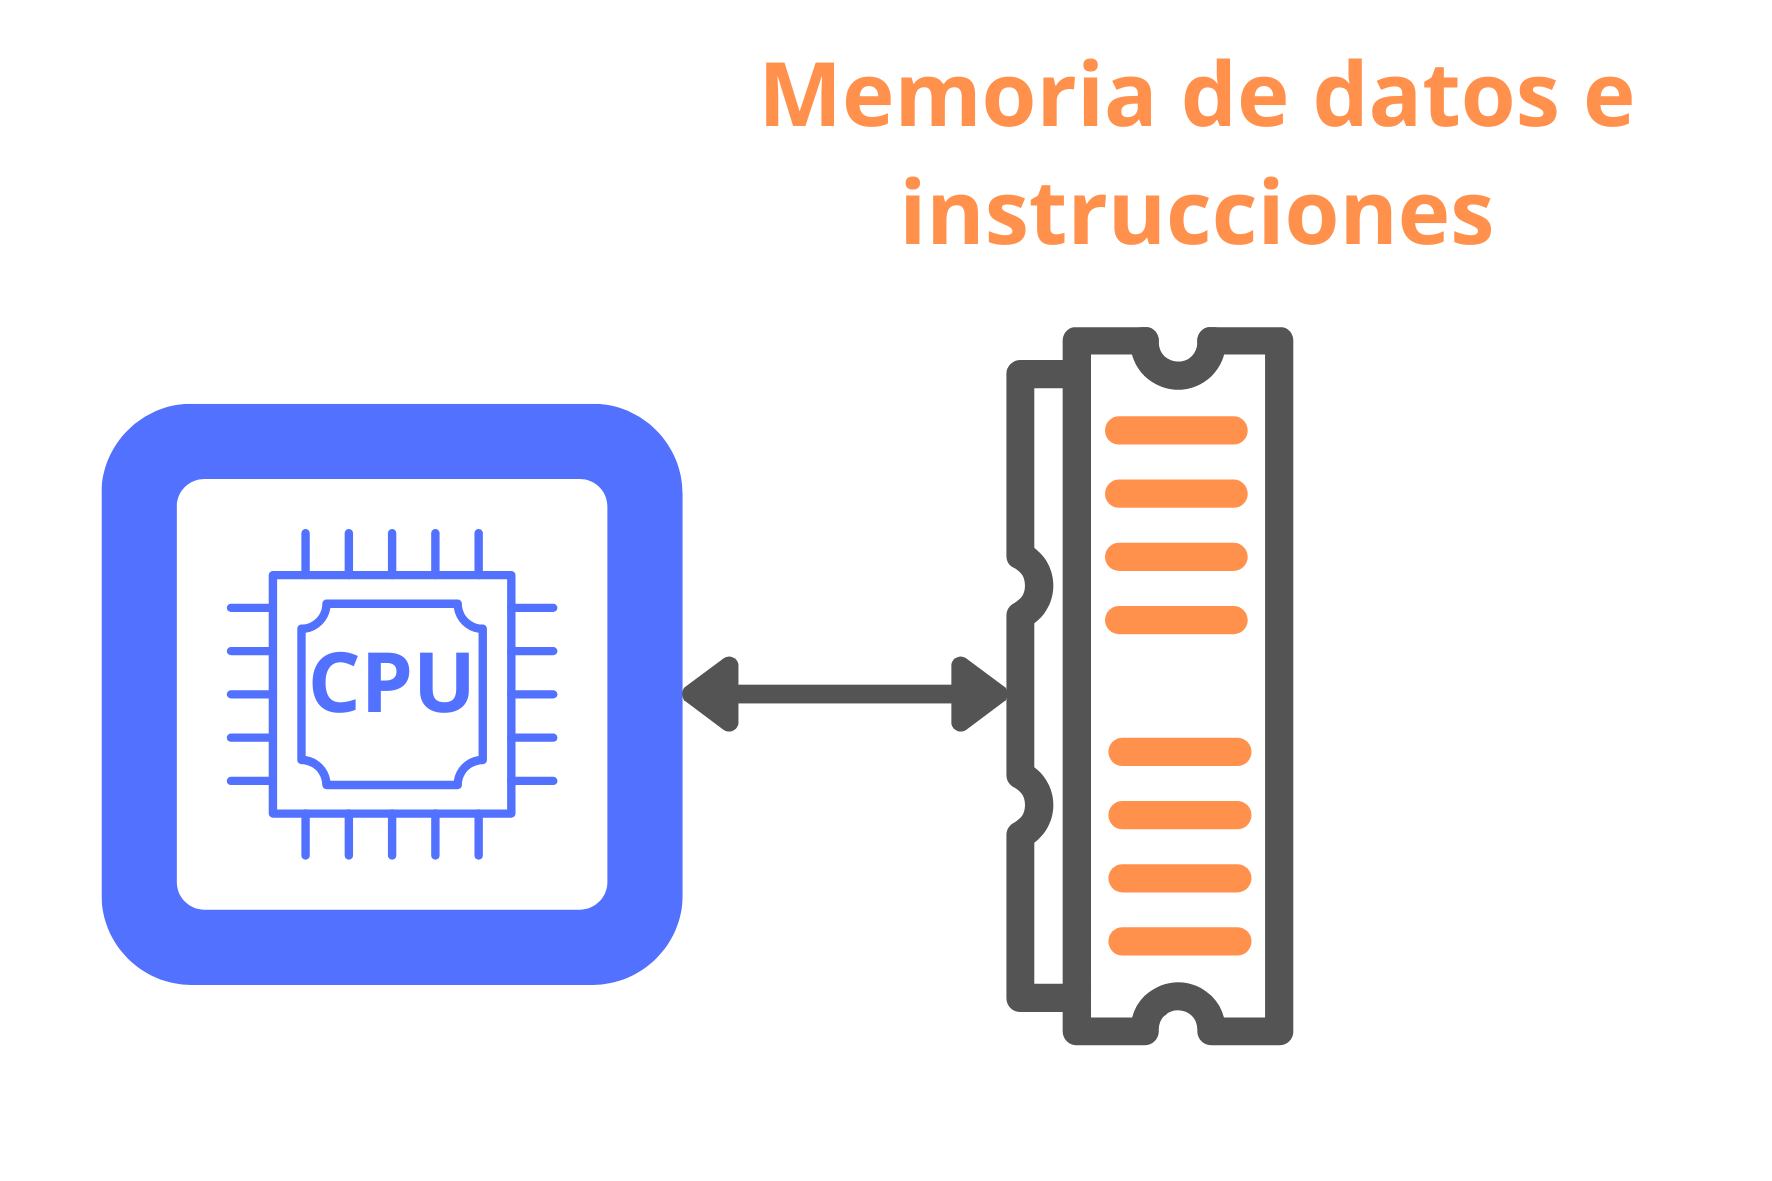
\includegraphics[width=0.85\linewidth]{images/vonneumann} 

}

\caption{Arquitectura Von Neumann}\label{fig:vonneumann}
\end{figure}

\hypertarget{arquitectura-harvard}{%
\subsection{Arquitectura Harvard}\label{arquitectura-harvard}}

Mientras la arquitectura Von Neumann se convertía en el paradigma dominante, paralelamente se desarrollaba un enfoque alternativo. La arquitectura Harvard tiene su origen en el diseño del Harvard Mark I, una computadora electromecánica desarrollada entre 1939 y 1944 durante la Segunda Guerra Mundial en la Universidad de Harvard bajo la dirección de Howard Aiken y con el apoyo de IBM \protect\hyperlink{ref-ceruzzi_history_2003}{{[}35{]}}, \protect\hyperlink{ref-williams1998history}{{[}36{]}}. El Harvard Mark I sentó las bases para un modelo arquitectónico diferente al de Von Neumann, caracterizado por una separación física entre instrucciones y datos.En este modelo, los datos y las instrucciones residen en memorias físicamente separadas, accedidas a través de buses independientes, lo cual mejora la eficiencia del procesamiento al eliminar la competencia por el bus entre instrucciones y datos. Esta organización evita el cuello de botella característico de Von Neumann y permite un acceso paralelo que incrementa el rendimiento en escenarios críticos para la eficiencia. A continuación, se presenta una comparación sistemática entre ambos modelos, a fin de comprender mejor sus implicancias técnicas y contextos de aplicación \protect\hyperlink{ref-tanenbaum_structured_2016}{{[}22{]}}. Debido a su eficiencia, esta arquitectura se ha adoptado ampliamente en sistemas embebidos, microcontroladores y procesadores de señal digital (DSP) \protect\hyperlink{ref-noergaard2012embedded}{{[}37{]}}.

\begin{figure}

{\centering 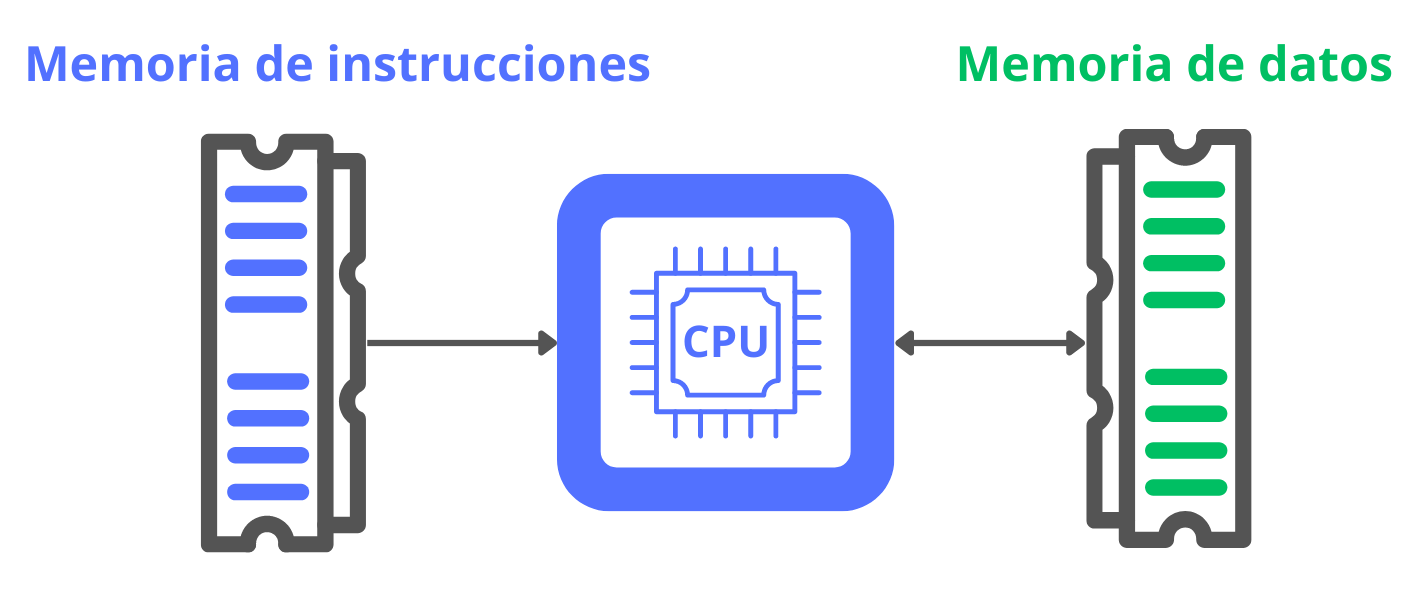
\includegraphics[width=0.85\linewidth]{images/harvard} 

}

\caption{Arquitectura Harvard}\label{fig:harvard}
\end{figure}

\hypertarget{comparativa-entre-von-neumann-y-harvard}{%
\subsection{Comparativa entre Von Neumann y Harvard}\label{comparativa-entre-von-neumann-y-harvard}}

Como señalan Stallings \protect\hyperlink{ref-stallings_computer_2021}{{[}14{]}} y Hennessy \protect\hyperlink{ref-hennessy2017computer}{{[}13{]}}, la arquitectura Von Neumann continúa siendo una alternativa predominante cuando se priorizan la simplicidad del diseño, la flexibilidad en la asignación de memoria y la compatibilidad con software de propósito general, como ocurre en muchas computadoras personales y servidores contemporáneos. En cambio, la arquitectura Harvard ha demostrado ventajas significativas en aplicaciones que demandan procesamiento en tiempo real y eficiencia energética, como dispositivos móviles, microcontroladores y entornos de control industrial. La elección entre ambas arquitecturas responde, en última instancia, a requerimientos específicos del sistema, ya sea por su complejidad, restricciones energéticas o necesidades de rendimiento paralelo.

Para una comparación más sistemática, se pueden establecer criterios como tipo de memoria, estructura de buses, capacidad de acceso paralelo, casos de uso representativos, ventajas y limitaciones.

\begin{table}[!h]
\centering
\caption{\label{tab:unnamed-chunk-1}Cuadro comparativo entre arquitecturas Von Neumann y Harvard}
\centering
\resizebox{\ifdim\width>\linewidth\linewidth\else\width\fi}{!}{
\begin{tabular}[t]{>{\raggedright\arraybackslash}p{4cm}|>{\raggedright\arraybackslash}p{5cm}>{\raggedright\arraybackslash}p{5cm}}
\toprule
\multicolumn{1}{>{\centering\arraybackslash}p{4cm}}{\cellcolor[HTML]{D3D3D3}{\textbf{Característica}}} & \multicolumn{1}{>{\centering\arraybackslash}p{5cm}}{\cellcolor[HTML]{D3D3D3}{\textbf{Von.Neumann}}} & \multicolumn{1}{>{\centering\arraybackslash}p{5cm}}{\cellcolor[HTML]{D3D3D3}{\textbf{Harvard}}}\\
\midrule
\textbf{Memoria} & Única para datos e instrucciones & Separada para datos e instrucciones\\
\textbf{Buses} & Bus compartido & Buses independientes\\
\textbf{Acceso simultáneo} & No & Sí\\
\textbf{Ejemplo típico} & Intel x86 & AVR, PIC\\
\textbf{Ventaja principal} & Diseño más simple & Mayor rendimiento\\
\addlinespace
\textbf{Limitación principal} & Cuello de botella & Diseño más complejo\\
\bottomrule
\end{tabular}}
\end{table}

Ambos modelos conceptuales han tenido una influencia decisiva en el diseño de arquitecturas contemporáneas. Mientras que el modelo Von Neumann ofrece un enfoque unificado que simplifica el desarrollo de software y hardware, la arquitectura Harvard destaca por su capacidad para mejorar el rendimiento mediante el acceso paralelo a instrucciones y datos. Esta distinción resulta crucial al analizar el diseño de arquitecturas modernas como x86, que constituye el foco de esta tesis. Comprender las implicancias de estas decisiones arquitectónicas es esencial para evaluar el impacto en el rendimiento, la eficiencia energética y la escalabilidad de los sistemas actuales.

El contraste entre estos dos modelos ha dado lugar a enfoques intermedios que buscan capitalizar las ventajas de ambos. Como resultado de esta evolución, emergen las denominadas arquitecturas híbridas, las cuales integran características de ambos modelos para optimizar el rendimiento y la flexibilidad del sistema.

\hypertarget{arquitecturas-huxedbridas}{%
\subsection{Arquitecturas híbridas}\label{arquitecturas-huxedbridas}}

Muchas arquitecturas contemporáneas implementan un enfoque híbrido, también conocido como arquitectura Harvard modificada. Este modelo emplea memorias separadas para datos e instrucciones a nivel microarquitectónico a menudo mediante la utilización de memorias caché de nivel 1 (L1) separadas para instrucciones y datos. No obstante, desde la perspectiva del programador, el modelo de memoria se mantiene unificado, facilitando el desarrollo de software sin exponer la complejidad del diseño interno. Esta dualidad permite optimizar la implementación física del procesador sin complicar el modelo de programación \protect\hyperlink{ref-hennessy2017computer}{{[}13{]}}, \protect\hyperlink{ref-stallings_computer_2021}{{[}14{]}}, \protect\hyperlink{ref-null_essentials_2014}{{[}27{]}}, \protect\hyperlink{ref-patterson_computer_2017}{{[}31{]}}.

\begin{figure}

{\centering 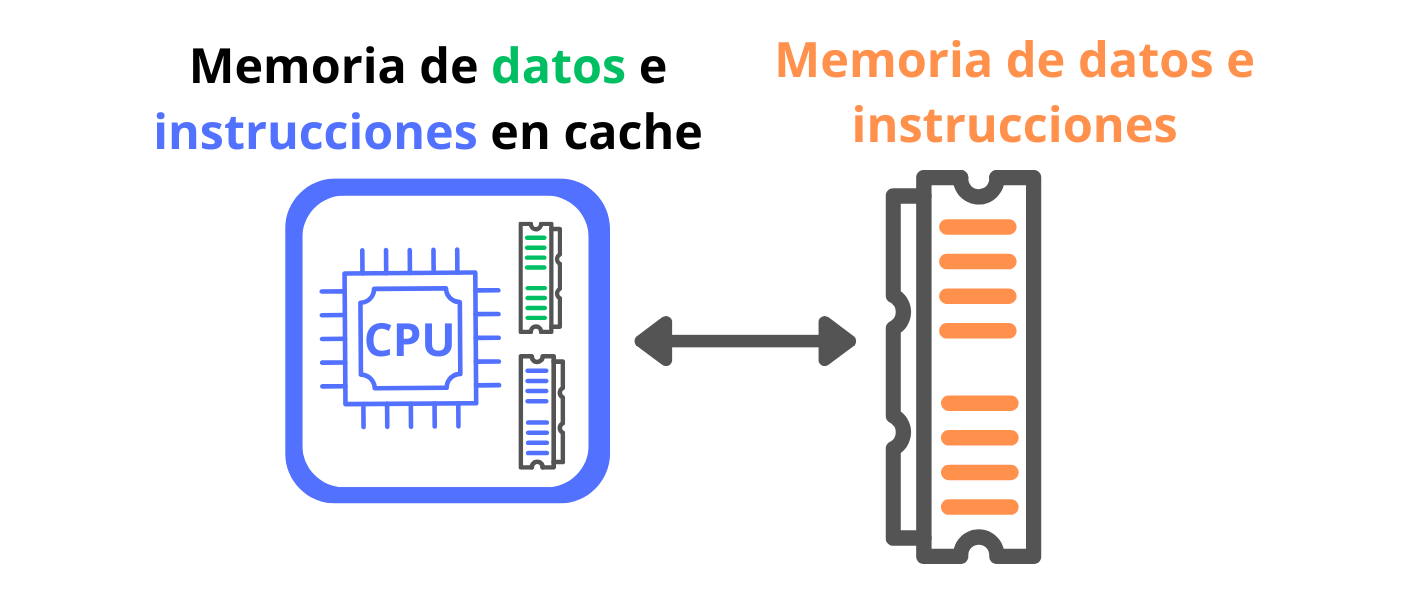
\includegraphics[width=0.85\linewidth]{images/hibrida} 

}

\caption{Arquitectura Híbridas}\label{fig:hibrida}
\end{figure}

Esta aproximación híbrida se implementa en arquitecturas modernas como ARM Cortex y los procesadores Intel Core, los cuales incorporan cachés separadas para instrucciones y datos con el objetivo de optimizar el rendimiento del pipeline, lo que facilita una mayor paralelización del procesamiento y reduce los conflictos en el acceso a memoria. A pesar de que el modelo de memoria visible para el programador se presenta como unificado, a nivel interno se implementan mecanismos característicos de la arquitectura Harvard, como el uso de memorias caché separadas para instrucciones y datos \protect\hyperlink{ref-arm2021architecture}{{[}38{]}}, \protect\hyperlink{ref-intel_microarchitecture_2021}{{[}39{]}}.

La adopción de arquitecturas híbridas, como la Harvard modificada, ha permitido a los diseñadores combinar la flexibilidad del modelo Von Neumann con la eficiencia del modelo Harvard. Esta convergencia no solo optimiza el rendimiento de los sistemas, sino que también responde a las exigencias contemporáneas en términos de consumo energético y capacidad de procesamiento paralelo. En este sentido, la distinción entre ambos modelos continúa siendo un eje conceptual clave para comprender la evolución de las arquitecturas modernas y su adaptación a diferentes escenarios tecnológicos.

En síntesis, la comprensión de las arquitecturas fundamentales ---Von Neumann, Harvard e híbridas--- resulta esencial para el desarrollo de herramientas de simulación efectivas en la enseñanza de arquitectura de computadoras. Los conceptos explorados en esta sección proporcionan los fundamentos conceptuales esenciales para el diseño y desarrollo de la herramienta de simulación propuesta en esta tesis.

\hypertarget{tipos-de-arquitecturas}{%
\section{Tipos de arquitecturas}\label{tipos-de-arquitecturas}}

El análisis de diversas arquitecturas de computadoras, y particularmente de sus repertorios de instrucciones (Instruction Set Architecture, ISA), es esencial para comprender sus ventajas, limitaciones y áreas de aplicación. Esta evaluación comparativa permite a los diseñadores y educadores seleccionar la ISA más adecuada para sus necesidades, considerando factores como la eficiencia energética, la complejidad del hardware, la compatibilidad y el soporte educativo.

Aunque arquitecturas como PowerPC, SPARC o MIPS desempeñaron un papel central en la evolución de la computación, su adopción ha disminuido significativamente en contextos industriales y académicos, debido al desplazamiento por plataformas con mayor soporte comercial y vigencia tecnológica \protect\hyperlink{ref-stallings_computer_2021}{{[}14{]}}. Su menor vigencia actual responde al surgimiento de arquitecturas más eficientes y con mejor respaldo comercial, como x86, ARM y RISC-V, que han captado la atención tanto del mercado como del ámbito educativo \protect\hyperlink{ref-hennessy2017computer}{{[}13{]}}, \protect\hyperlink{ref-waterman_risc-v_2014}{{[}25{]}}, \protect\hyperlink{ref-null_essentials_2014}{{[}27{]}}, \protect\hyperlink{ref-arm_evolution_2025}{{[}40{]}}. Por ello, esta sección se enfoca en aquellas arquitecturas que mantienen relevancia comercial o presentan un valor pedagógico significativo en el desarrollo de simuladores educativos.

\hypertarget{arquitectura-x86}{%
\subsection{Arquitectura x86}\label{arquitectura-x86}}

La arquitectura x86, desarrollada inicialmente por Intel, ha dominado el mercado de computadoras de escritorio y servidores durante décadas, gracias a su evolución constante y soporte del ecosistema de software \protect\hyperlink{ref-hennessy2017computer}{{[}13{]}}. Su conjunto de instrucciones (ISA, por sus siglas en inglés Instruction Set Architecture) incluye una amplia gama de operaciones, lo que otorga flexibilidad, aunque complica el diseño del hardware. Este equilibrio entre compatibilidad y rendimiento hace que x86 sea una opción preferida para entornos donde la capacidad de procesamiento es prioritaria, como en servidores y estaciones de trabajo \protect\hyperlink{ref-hennessy2017computer}{{[}13{]}}, \protect\hyperlink{ref-intel_whitepaper_2023}{{[}41{]}}.

\hypertarget{arquitectura-arm}{%
\subsection{Arquitectura ARM}\label{arquitectura-arm}}

Reconocida por su alta eficiencia energética, la arquitectura ARM es la columna vertebral de dispositivos móviles y sistemas embebidos. Basada en el paradigma de conjunto de instrucciones reducidas (RISC), ARM simplifica el diseño del hardware y optimiza el consumo energético, características que la posicionan como una opción preferente para aplicaciones como smartphones y tablets. Aunque su rendimiento máximo en tareas de cómputo intensivo suele ser inferior al de x86, su equilibrio entre eficiencia energética y capacidad computacional resulta decisivo en mercados donde la autonomía y la disipación térmica son factores críticos, como los dispositivos móviles y el IoT \protect\hyperlink{ref-patterson_computer_2014}{{[}28{]}}, \protect\hyperlink{ref-arm_evolution_2025}{{[}40{]}}.

\hypertarget{arquitectura-risc-v}{%
\subsection{Arquitectura RISC-V}\label{arquitectura-risc-v}}

Como arquitectura de código abierto, RISC-V ofrece una alternativa personalizable a los modelos propietarios, destacándose en entornos académicos y de desarrollo especializado. Su ISA flexible permite a los desarrolladores personalizar sistemas según necesidades específicas, haciéndola especialmente atractiva para investigación, educación y aplicaciones embebidas. Basada en principios RISC, RISC-V combina eficiencia energética con un diseño de hardware simplificado, y su creciente ecosistema la posiciona como una fuerte competidora frente a arquitecturas establecidas como ARM. No obstante, RISC-V enfrenta desafíos para su adopción masiva, en parte debido a la falta de estándares unificados, la fragmentación de su ecosistema y la limitada presencia de proveedores comerciales consolidados, lo que dificulta su despliegue en entornos productivos críticos.\protect\hyperlink{ref-hennessy2017computer}{{[}13{]}}, \protect\hyperlink{ref-waterman_risc-v_2014}{{[}25{]}}, \protect\hyperlink{ref-harris2015digital}{{[}26{]}}, \protect\hyperlink{ref-patterson2016computer}{{[}42{]}}.

\hypertarget{comparativa-entre-arquitecturas}{%
\subsection{Comparativa entre arquitecturas}\label{comparativa-entre-arquitecturas}}

Las características distintivas de cada arquitectura condicionan su idoneidad para diversas aplicaciones. Por ejemplo, mientras x86 sobresale en entornos de alto rendimiento, ARM domina en dispositivos móviles gracias a su eficiencia energética. Por su parte, arquitecturas como RISC-V han encontrado aplicaciones relevantes en sistemas embebidos, plataformas educativas y diseños personalizados, aunque su presencia comercial difiere notablemente. La selección adecuada de una arquitectura impacta significativamente en el éxito de un proyecto, desde el diseño hasta su implementación final. Además, comprender las diferencias entre estas arquitecturas, en particular sus repertorios de instrucciones y principios de diseño, resulta fundamental en el ámbito educativo, dado que facilita el desarrollo de herramientas didácticas que simulan sus principios operativos y ayudan a los estudiantes a visualizar el funcionamiento real de los sistemas computacionales \protect\hyperlink{ref-patterson_computer_2014}{{[}28{]}}, \protect\hyperlink{ref-arm_evolution_2025}{{[}40{]}}.

\begin{table}[!h]
\centering
\caption{\label{tab:aplicacionessimulacion}Aplicaciones de la simulación en distintos sectores}
\centering
\resizebox{\ifdim\width>\linewidth\linewidth\else\width\fi}{!}{
\fontsize{10}{12}\selectfont
\begin{tabular}[t]{>{\raggedright\arraybackslash}p{4cm}|>{\raggedright\arraybackslash}p{4cm}>{\raggedright\arraybackslash}p{4cm}}
\toprule
\multicolumn{1}{>{\centering\arraybackslash}p{4cm}}{\cellcolor[HTML]{D3D3D3}{\textbf{Sector}}} & \multicolumn{1}{>{\centering\arraybackslash}p{4cm}}{\cellcolor[HTML]{D3D3D3}{\textbf{Aplicación}}} & \multicolumn{1}{>{\centering\arraybackslash}p{4cm}}{\cellcolor[HTML]{D3D3D3}{\textbf{Beneficio principal}}}\\
\midrule
\textbf{Automotriz} & Pruebas de colisión virtuales & Reducción de costos y aumento de seguridad\\
\addlinespace[10pt]
\textbf{Aeroespacial} & Simuladores de vuelo & Entrenamiento sin riesgo\\
\addlinespace[10pt]
\textbf{Medicina} & Simulación de cirugías & Entrenamiento sin comprometer pacientes\\
\addlinespace[10pt]
\textbf{Educación} & Simuladores para arquitectura de computadoras & Comprensión de procesos abstractos\\
\addlinespace[10pt]
\bottomrule
\end{tabular}}
\end{table}

En el contexto de la enseñanza de arquitectura de computadoras, estas arquitecturas permiten abordar distintos niveles de complejidad y estilos de diseño, lo que resulta clave para la construcción de simuladores educativos efectivos.

\hypertarget{repertorio-de-instrucciones}{%
\section{Repertorio de instrucciones}\label{repertorio-de-instrucciones}}

El repertorio de instrucciones, o Instruction Set Architecture (ISA), es el conjunto de operaciones que un procesador puede ejecutar, incluyendo su representación binaria y el conjunto de reglas que definen la interacción entre el software y el hardware. El ISA define la interfaz entre el hardware y el software, abarcando instrucciones aritméticas, lógicas, de control y de manipulación de datos, así como los modos de direccionamiento y los formatos de instrucción. Por su influencia directa en el rendimiento, la eficiencia energética y la versatilidad del sistema, el ISA constituye un componente esencial en el diseño de arquitecturas de computadoras \protect\hyperlink{ref-hennessy2017computer}{{[}13{]}}, \protect\hyperlink{ref-stallings_computer_2021}{{[}14{]}}, \protect\hyperlink{ref-null_essentials_2014}{{[}27{]}}.

\hypertarget{caracteruxedsticas-clave-del-isa}{%
\subsection{Características clave del ISA}\label{caracteruxedsticas-clave-del-isa}}

Entre las características fundamentales a considerar en el diseño de un repertorio de instrucciones se encuentran las siguientes \protect\hyperlink{ref-hennessy2017computer}{{[}13{]}}:

\begin{itemize}
\tightlist
\item
  \textbf{Tipos de operandos}: representan los datos que las instrucciones pueden manipular, como enteros, números en punto flotante, caracteres y direcciones de memoria. Un ISA eficiente debe soportar una amplia variedad de operandos para maximizar su versatilidad.
\item
  \textbf{Tipos de operaciones}: incluyen las operaciones que el procesador puede realizar, como aritméticas (suma, resta), lógicas (AND, OR), de control (saltos, llamadas a subrutinas) y de manipulación de datos (almacenamiento, carga). Diversos autores destacan que un ISA bien diseñado debe lograr un equilibrio entre funcionalidad, simplicidad y eficiencia de implementación, aspectos fundamentales en el diseño de arquitecturas modernas \protect\hyperlink{ref-hennessy2017computer}{{[}13{]}}, \protect\hyperlink{ref-null_essentials_2014}{{[}27{]}}.
\item
  \textbf{Modos de direccionamiento}: determinan cómo se especifican los operandos en las instrucciones. Entre los modos más comunes se encuentran el inmediato, directo, indirecto, mediante registros, con desplazamiento y basado en pila. Cada uno ofrece distintos niveles de eficiencia, flexibilidad y complejidad, siendo fundamentales para optimizar el acceso a datos y la ejecución de instrucciones.
\item
  \textbf{Formato de las instrucciones}: que definen las reglas para acceder a los operandos dentro de las instrucciones, se exploran con mayor detalle en la siguiente subsección.
\end{itemize}

\begin{figure}

{\centering 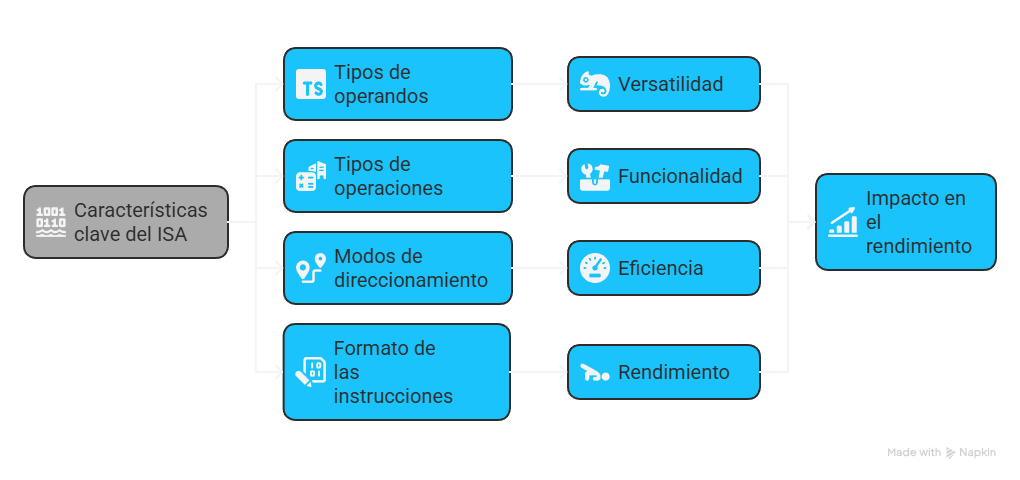
\includegraphics[width=1\linewidth]{images/isa} 

}

\caption{Características repertorio de instrucciones}\label{fig:repInstCaracteristicas}
\end{figure}

El diseño de un repertorio de instrucciones eficiente y versátil es un desafío complejo que requiere un equilibrio entre funcionalidad, rendimiento y facilidad de uso. La selección adecuada de operandos, operaciones y modos de direccionamiento, junto con un formato de instrucción bien estructurado, son aspectos fundamentales para lograr una arquitectura de computadoras efectiva y adaptable a diversas aplicaciones. Estas características no solo definen las capacidades funcionales de un procesador, sino que también condicionan la manera en que las instrucciones interactúan con la memoria y los registros. A continuación, se profundiza en los modos de direccionamiento, uno de los elementos que más influye en la flexibilidad y eficiencia del repertorio de instrucciones.

\hypertarget{modos-de-direccionamiento}{%
\subsection{Modos de direccionamiento}\label{modos-de-direccionamiento}}

Los modos de direccionamiento definen los mecanismos mediante los cuales una instrucción especifica la ubicación de sus operandos, permitiendo así al procesador acceder a los datos en memoria o registros en tiempo de ejecución. A continuación, se describen los modos de direccionamiento más comúnmente implementados en las arquitecturas modernas \protect\hyperlink{ref-hennessy2017computer}{{[}13{]}}, \protect\hyperlink{ref-stallings_computer_2021}{{[}14{]}}:

\begin{enumerate}
\def\labelenumi{\alph{enumi})}
\tightlist
\item
  \textbf{Inmediato}: el operando está directamente incluido en la instrucción, permitiendo acceso rápido a valores constantes. Es eficiente para operaciones simples, aunque limitado a operandos pequeños.
\item
  \textbf{Directo}: la instrucción contiene la dirección de memoria del operando. Es fácil de usar, pero está restringido por el rango de direcciones accesibles.
\item
  \textbf{Indirecto}: la instrucción apunta a una dirección que contiene la ubicación real del operando, lo que amplía el rango de direcciones a costa de un acceso adicional a memoria.
\item
  \textbf{Registro}: el operando se encuentra en un registro del procesador, proporcionando acceso extremadamente rápido, pero limitado por la cantidad de registros disponibles.
\item
  \textbf{Registro Indirecto}: similar al modo indirecto, pero la dirección efectiva se obtiene a partir del contenido de un registro, lo que ofrece un buen equilibrio entre velocidad de acceso y capacidad de direccionamiento.
\item
  \textbf{Con Desplazamiento}: combina una dirección base con un valor de desplazamiento, ideal para estructuras como arrays y matrices.
\item
  \textbf{Pila}: el operando está en la parte superior de la pila, útil para gestionar subrutinas y el paso de parámetros.
\end{enumerate}

Para complementar la descripción anterior, la Figura \ref{fig:ModDir} presenta una representación esquemática de los modos de direccionamiento, mostrando gráficamente cómo se calcula la dirección efectiva (EA) en cada caso \protect\hyperlink{ref-stallings_computer_2021}{{[}14{]}}.

\begin{figure}

{\centering 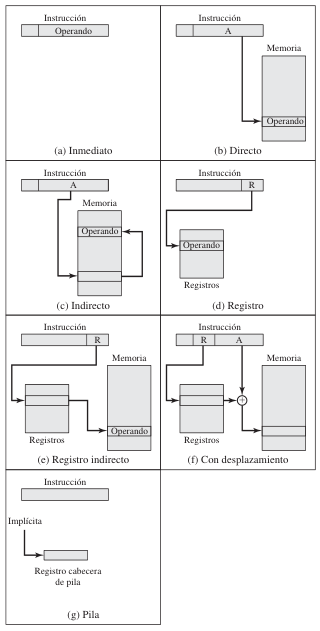
\includegraphics[width=0.6\linewidth]{images/modosdireccionamiento} 

}

\caption{Modos de direccionamiento }\label{fig:ModDir}
\end{figure}

\begin{itemize}
\tightlist
\item
  A = contenido de un campo de dirección en la instrucción
\item
  R = contenido de un campo de dirección en la instrucción que referencia a un registro
\item
  EA = dirección real (efectiva) de la posición que contiene el operando que se referencia
\end{itemize}

La tabla \ref{tab:tabmoddir} detalla el cálculo de la dirección para cada modo de direccionamiento.

\begin{table}[!h]
\centering
\caption{\label{tab:tabmoddir}Modos de direccionamiento básicos}
\centering
\resizebox{\ifdim\width>\linewidth\linewidth\else\width\fi}{!}{
\fontsize{10}{12}\selectfont
\begin{tabular}[t]{>{\raggedright\arraybackslash}p{4cm}|>{\raggedright\arraybackslash}p{4cm}>{\raggedright\arraybackslash}p{4cm}>{\raggedright\arraybackslash}p{4cm}}
\toprule
\multicolumn{1}{>{\centering\arraybackslash}p{4cm}}{\cellcolor[HTML]{D3D3D3}{\textbf{Modo}}} & \multicolumn{1}{>{\centering\arraybackslash}p{4cm}}{\cellcolor[HTML]{D3D3D3}{\textbf{Algoritmo}}} & \multicolumn{1}{>{\centering\arraybackslash}p{4cm}}{\cellcolor[HTML]{D3D3D3}{\textbf{Ventaja}}} & \multicolumn{1}{>{\centering\arraybackslash}p{4cm}}{\cellcolor[HTML]{D3D3D3}{\textbf{Desventaja}}}\\
\midrule
\textbf{Inmediato} & Operando ← A & No referencia a memoria & Operando de magnitud limitada\\
\addlinespace[10pt]
\textbf{Directo} & EA ← A & Es sencillo & Espacio de direcciones limitado\\
\addlinespace[10pt]
\textbf{Indirecto} & EA ← (A) & Espacio de direcciones grande & Referencias múltiples a memoria\\
\addlinespace[10pt]
\textbf{Registro} & EA ← R & No referencia a memoria & Número limitado de registros\\
\addlinespace[10pt]
\textbf{Indirecto con registro} & EA ← (R) & Espacio de direcciones grande & Referencia extra a memoria\\
\addlinespace[10pt]
\addlinespace
\textbf{Con desplazamiento} & EA ← A + (R) & Flexibilidad & Complejidad\\
\addlinespace[10pt]
\textbf{Pila} & EA ← puntero de pila & No referencia a memoria & Aplicabilidad limitada\\
\addlinespace[10pt]
\bottomrule
\end{tabular}}
\end{table}

\hypertarget{formato-de-las-instrucciones}{%
\subsection{Formato de las instrucciones}\label{formato-de-las-instrucciones}}

El formato de las instrucciones especifica la disposición y codificación de los elementos que conforman una instrucción, como el código de operación (opcode), los operandos, los modos de direccionamiento y otros campos auxiliares. Esta organización impacta directamente en la facilidad de decodificación y en el rendimiento del procesador. Este formato afecta la rapidez de decodificación y la eficiencia general del procesador \protect\hyperlink{ref-hennessy2017computer}{{[}13{]}}, \protect\hyperlink{ref-tanenbaum_structured_2016}{{[}22{]}}:

\begin{itemize}
\tightlist
\item
  \textbf{Longitud de la instrucción}: puede ser fija o variable. Las instrucciones de longitud fija permiten una decodificación más rápida y simplifican la lógica de control del procesador. En cambio, las instrucciones de longitud variable permiten una codificación más eficiente del espacio de memoria, a costa de una mayor complejidad en la etapa de decodificación.
\item
  \textbf{Cantidad de operandos}: las instrucciones pueden trabajar con diferentes números de operandos (de 0 a 3 o más). Una mayor cantidad de operandos incrementa la expresividad de las instrucciones, pero también puede derivar en una mayor complejidad de codificación y en un mayor uso de recursos del procesador.
\item
  \textbf{Campos de instrucción}: incluyen el opcode y campos adicionales como operandos, modos de direccionamiento y flags de condición. Estos campos determinan cuántas y qué tipo de operaciones puede ejecutar el procesador en un ciclo de reloj.
\end{itemize}

La Figura \ref{fig:forminst} muestra un ejemplo representativo de formato de instrucción, donde se visualizan los campos que la componen y su disposición en el código binario.

\begin{figure}

{\centering 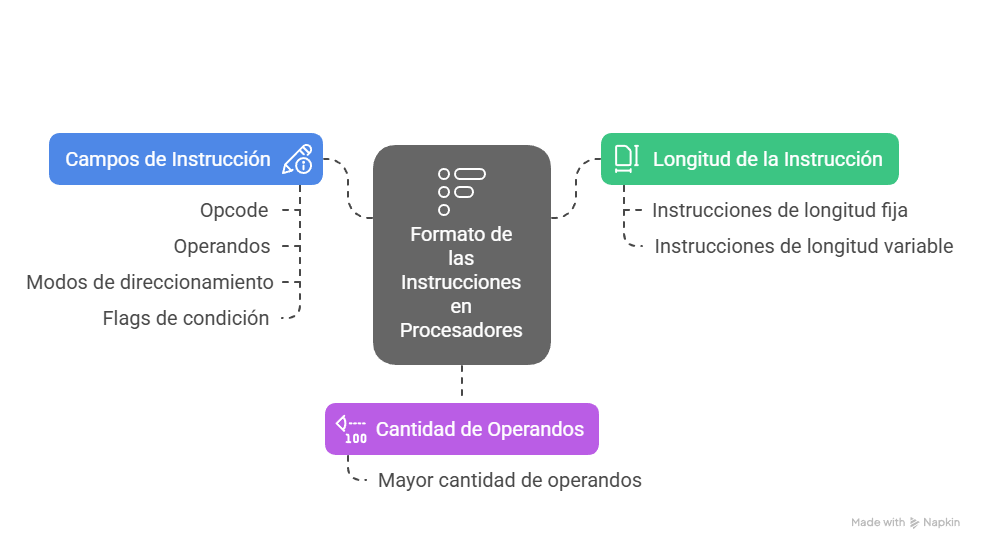
\includegraphics[width=1\linewidth]{images/formatoinst} 

}

\caption{Formato de instrucciones }\label{fig:forminst}
\end{figure}

\hypertarget{comparativa-de-repertorios-de-instrucciones-reales}{%
\subsection{Comparativa de repertorios de instrucciones reales}\label{comparativa-de-repertorios-de-instrucciones-reales}}

La siguiente tabla \ref{tab:comparativaISA} resume las características principales de los repertorios de instrucciones en tres arquitecturas ampliamente utilizadas: x86, ARM y RISC-V. Se consideran aspectos como la longitud de las instrucciones, la cantidad de operandos, su complejidad y los modos de direccionamiento que permiten.

\begin{table}[!h]
\centering
\caption{\label{tab:comparativaISA}Comparativa de repertorios de instrucciones reales}
\centering
\resizebox{\ifdim\width>\linewidth\linewidth\else\width\fi}{!}{
\begin{tabular}[t]{>{}l|>{\raggedright\arraybackslash}p{4cm}>{\raggedright\arraybackslash}p{4cm}>{\raggedright\arraybackslash}p{4cm}>{\raggedright\arraybackslash}p{4cm}}
\toprule
\multicolumn{1}{c}{\cellcolor[HTML]{D3D3D3}{\textbf{Arquitectura}}} & \multicolumn{1}{>{\centering\arraybackslash}p{4cm}}{\cellcolor[HTML]{D3D3D3}{\textbf{Longitud instrucción}}} & \multicolumn{1}{>{\centering\arraybackslash}p{4cm}}{\cellcolor[HTML]{D3D3D3}{\textbf{Nº operandos}}} & \multicolumn{1}{>{\centering\arraybackslash}p{4cm}}{\cellcolor[HTML]{D3D3D3}{\textbf{Tipos de operandos}}} & \multicolumn{1}{>{\centering\arraybackslash}p{4cm}}{\cellcolor[HTML]{D3D3D3}{\textbf{Modos de direccionamiento}}}\\
\midrule
\textbf{x86} & Variable & 0–3+ & Complejos & Muchos\\
\textbf{ARM} & Fija (32 bits) & 3 & Simples & Limitados\\
\textbf{RISC-V} & Fija (32 bits) & 3 & Simples & Extensible\\
\bottomrule
\end{tabular}}
\end{table}

\hypertarget{filosofuxedas-cisc-y-risc}{%
\section{Filosofías CISC y RISC}\label{filosofuxedas-cisc-y-risc}}

El diseño del repertorio de instrucciones es una decisión estratégica clave en la arquitectura de procesadores, ya que determina no solo el rendimiento del sistema, sino también la complejidad del hardware y del software, en particular del compilador. Dos de las filosofías más influyentes en este campo son \textbf{CISC (Complex Instruction Set Computing)} y \textbf{RISC (Reduced Instruction Set Computing)}. Mientras que \textbf{CISC} prioriza la reducción del número de instrucciones necesarias para realizar tareas complejas mediante operaciones multifuncionales, \textbf{RISC} simplifica el conjunto de instrucciones con el objetivo de maximizar la velocidad y la eficiencia energética. En esta sección se analizan ambos enfoques y sus implicaciones en el diseño de procesadores \protect\hyperlink{ref-hennessy2017computer}{{[}13{]}}, \protect\hyperlink{ref-patterson_computer_2014}{{[}28{]}}.

El debate entre las filosofías CISC y RISC se remonta a fines de la década de 1970, cuando se comenzaron a cuestionar los beneficios reales de los repertorios de instrucciones complejos. Mientras las primeras generaciones de computadoras buscaban reducir el número de instrucciones por programa, investigaciones posteriores demostraron que un conjunto reducido y eficiente de instrucciones podía mejorar significativamente el rendimiento al simplificar la ejecución y optimizar el uso del hardware.

La evolución de los procesadores ha llevado a un enfoque más equilibrado, donde las arquitecturas modernas combinan elementos de ambas filosofías. Las arquitecturas modernas tienden a incorporar elementos de ambas filosofías. Por ejemplo, x86 adopta técnicas de ejecución interna propias de RISC para aumentar su rendimiento, mientras que procesadores RISC como ARM han introducido extensiones complejas para tareas específicas, acercándose parcialmente al enfoque CISC \protect\hyperlink{ref-hennessy2017computer}{{[}13{]}}, \protect\hyperlink{ref-patterson_computer_2014}{{[}28{]}}.

\hypertarget{cisc}{%
\subsection{CISC}\label{cisc}}

Las arquitecturas \textbf{CISC}, como la \textbf{x86}, se caracterizan por su enfoque en reducir el número de instrucciones requeridas para completar operaciones complejas. Esto se logra mediante la inclusión de instrucciones que combinan múltiples operaciones en un solo ciclo. Como resultado, los programadores necesitan escribir menos líneas de código para alcanzar un objetivo específico.

Sin embargo, este diseño implica ciertas desventajas. La \textbf{decodificación} y \textbf{ejecución} de instrucciones CISC requiere un hardware considerablemente más complejo, y las instrucciones de longitud variable, típicas de estas arquitecturas, pueden aumentar el tiempo de decodificación. Esto genera cuellos de botella en el pipeline y limita el rendimiento.

Un ejemplo representativo es la arquitectura x86, que ha incorporado técnicas internas de ejecución similares a RISC ---como la descomposición de instrucciones mediante microcódigo--- con el fin de mejorar el rendimiento sin abandonar su repertorio complejo. Utiliza microcódigo para descomponer las instrucciones complejas en operaciones más simples, parecidas a las de un procesador RISC. Aunque esta estrategia mejora la eficiencia de ejecución en algunos casos, el diseño sigue siendo más costoso en términos de consumo energético y complejidad \protect\hyperlink{ref-patterson_computer_2014}{{[}28{]}}.

En consecuencia, el diseño del repertorio de instrucciones ---incluyendo operaciones, modos de direccionamiento y formatos--- constituye la interfaz crítica entre hardware y software, afectando tanto la eficiencia de ejecución como la expresividad de los programas. Su diseño influye directamente en la eficiencia del procesamiento y en la forma en que los programas interactúan con la arquitectura subyacente, lo que refuerza su relevancia en el estudio de la arquitectura de computadoras.

\hypertarget{RISC}{%
\subsection{RISC}\label{RISC}}

Las arquitecturas basadas en RISC, en contraste con CISC, se caracterizan por emplear instrucciones simples y de longitud fija. Esta simplificación facilita la decodificación y permite que muchas instrucciones se ejecuten en un solo ciclo de reloj. Además, esta filosofía favorece la implementación de técnicas avanzadas como el pipelining y la predicción de ramas, optimizando así el rendimiento.

A nivel de hardware, RISC prioriza la eficiencia energética, una característica crucial en dispositivos móviles y sistemas embebidos. Por ello, procesadores como los basados en ARM han dominado estos mercados, especialmente en dispositivos móviles, debido a su bajo consumo energético. La simplicidad y el bajo CPI (ciclos por instrucción) han sido factores determinantes en su adopción \protect\hyperlink{ref-hennessy2017computer}{{[}13{]}}.

\hypertarget{comparativa-entre-cisc-y-risc}{%
\subsection{Comparativa entre CISC y RISC}\label{comparativa-entre-cisc-y-risc}}

Las diferencias entre CISC y RISC son evidentes tanto a nivel de diseño como de implementación. En las arquitecturas RISC, las instrucciones tienen una longitud fija, lo que simplifica la decodificación, reduce la latencia y mejora la predictibilidad del rendimiento. Además, este formato mejora la eficiencia del uso de la memoria caché, al ocupar menos espacio y facilitar accesos más rápidos.

En cambio, las arquitecturas CISC, como x86, emplean instrucciones de longitud variable, lo que les permite ofrecer una mayor flexibilidad y un repertorio más amplio de operaciones. Sin embargo, esta flexibilidad conlleva un mayor tiempo de decodificación y una complejidad adicional en la implementación del pipeline. Esto puede causar problemas como interrupciones en el flujo debido a errores de predicción de ramas, aunque se mitiguen mediante técnicas avanzadas como la predicción dinámica de saltos y el prefetching \protect\hyperlink{ref-tanenbaum_structured_2016}{{[}22{]}}.

Por ejemplo, en RISC, los modos de direccionamiento son simples y permiten un acceso más rápido a los operandos, reduciendo la latencia en el pipeline \protect\hyperlink{ref-stallings_computer_2021}{{[}14{]}}. En CISC, los modos de direccionamiento más complejos proporcionan flexibilidad a costa de una mayor latencia, lo que impacta negativamente en el rendimiento general del sistema.

\hypertarget{ejemplos-de-instrucciones}{%
\subsubsection{Ejemplos de instrucciones}\label{ejemplos-de-instrucciones}}

Para ilustrar la diferencia entre ambas filosofías, se presenta el siguiente ejemplo: cargar dos valores de memoria, sumarlos y almacenar el resultado en una dirección de memoria.

RISC:

\begin{lstlisting}
  ; Carga el valor inmediato 10 en el registro R0
  LOAD R1, [mem1]    # Cargar el valor de mem1 en el registro R1
  LOAD R2, [mem2]    # Cargar el valor de mem2 en el registro R2
  ADD  R3, R1, R2    # Sumar los valores en los registros R1 y R2, guardar en R3
  STORE R3, [mem1]   # Guardar el resultado en mem1
  \end{lstlisting}

CISC:

\begin{lstlisting}
  MOV EAX, [mem1]    # Cargar el valor de mem1 en el registro EAX
  ADD EAX, [mem2]    # Sumar el valor de mem2 con EAX
  MOV [mem1], EAX    # Guardar el resultado de la suma de vuelta en mem1
  \end{lstlisting}

La tabla \ref{tab:ciscrisc} sintetiza las principales diferencias estructurales y operativas entre las filosofías CISC y RISC, destacando sus implicancias en el diseño del hardware y el rendimiento general del sistema.

\begin{table}[!h]
\centering
\caption{\label{tab:ciscrisc}Comparativa entre CISC y RISC}
\centering
\resizebox{\ifdim\width>\linewidth\linewidth\else\width\fi}{!}{
\fontsize{10}{12}\selectfont
\begin{tabular}[t]{>{\raggedright\arraybackslash}p{6cm}|>{\raggedright\arraybackslash}p{5cm}>{\raggedright\arraybackslash}p{5cm}}
\toprule
\multicolumn{1}{>{\centering\arraybackslash}p{6cm}}{\cellcolor[HTML]{D3D3D3}{\textbf{Aspecto}}} & \multicolumn{1}{>{\centering\arraybackslash}p{5cm}}{\cellcolor[HTML]{D3D3D3}{\textbf{CISC}}} & \multicolumn{1}{>{\centering\arraybackslash}p{5cm}}{\cellcolor[HTML]{D3D3D3}{\textbf{RISC}}}\\
\midrule
\textbf{Objetivo principal} & Minimizar el número de instrucciones para operaciones complejas & Simplificar el conjunto de instrucciones para optimizar velocidad y eficiencia energética\\
\addlinespace[10pt]
\textbf{Tipo de instrucciones} & Instrucciones complejas, longitud variable & Instrucciones simples, longitud fija\\
\addlinespace[10pt]
\textbf{Decodificación y ejecución} & Requiere hardware más complejo, posibles cuellos de botella en el pipeline & Decodificación más sencilla, facilita el uso de técnicas avanzadas como pipelining\\
\addlinespace[10pt]
\textbf{Longitud de instrucciones} & Longitud variable, puede aumentar el tiempo de decodificación & Longitud fija, simplifica la decodificación y mejora la predictibilidad del rendimiento\\
\addlinespace[10pt]
\textbf{Eficiencia energética} & Menor eficiencia energética en comparación con RISC & Mayor eficiencia energética, especialmente en dispositivos móviles\\
\addlinespace[10pt]
\addlinespace
\textbf{Modos de direccionamiento} & Flexibilidad a costa de mayor latencia & Acceso más rápido a los operandos, menor latencia\\
\addlinespace[10pt]
\bottomrule
\end{tabular}}
\end{table}

\hypertarget{convergencia-de-filosofuxedas}{%
\subsubsection{Convergencia de filosofías}\label{convergencia-de-filosofuxedas}}

A pesar de sus diferencias, las arquitecturas modernas tienden a integrar características de ambas filosofías. Por ejemplo, los procesadores x86 adoptan técnicas propias de RISC para mejorar la eficiencia energética y el rendimiento. Esta convergencia refleja cómo los avances en diseño de procesadores buscan combinar lo mejor de cada enfoque, maximizando la flexibilidad y la eficiencia para adaptarse a las necesidades actuales y futuras del mercado.

La Figura \ref{fig:convergen} muestras la convergencia entre estas dos filosofías:

\begin{figure}

{\centering 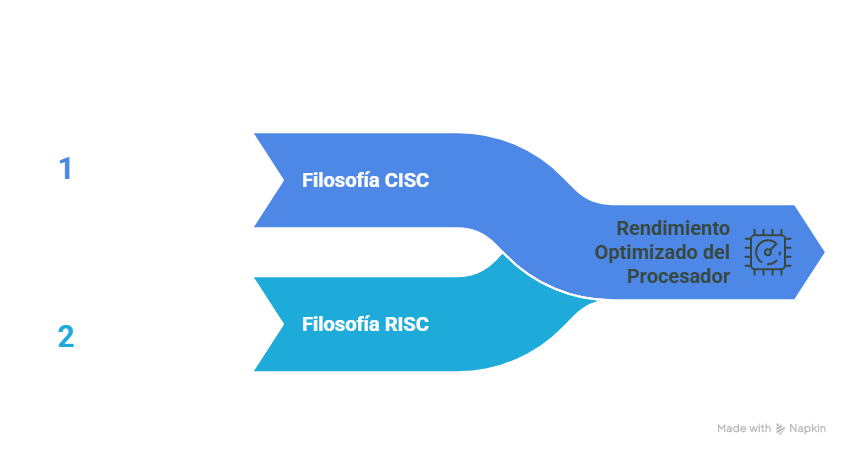
\includegraphics[width=1\linewidth]{images/convergen} 

}

\caption{Convergencia de filosofías}\label{fig:convergen}
\end{figure}

En síntesis, las filosofías CISC y RISC representan enfoques contrastantes pero complementarios en el diseño de arquitecturas de procesadores. Su comprensión no solo es esencial para analizar el rendimiento y la eficiencia energética de los sistemas modernos, sino también para formar una base sólida en la enseñanza de arquitectura de computadoras, especialmente en contextos donde se emplean simuladores didácticos.

\hypertarget{arquitectura-x86-1}{%
\section{Arquitectura x86}\label{arquitectura-x86-1}}

La arquitectura x86, reconocida por su amplia adopción en computadoras personales, estaciones de trabajo y servidores, se introdujo en 1978 con el procesador Intel 8086, basado en una arquitectura de 16 bits. Desde entonces, ha evolucionado en capacidad y complejidad, con hitos clave como la introducción del Intel 80386 (32 bits) en 1985 y la extensión a 64 bits con AMD64 en 2003. Esta evolución ha permitido mejoras significativas en el rendimiento, el direccionamiento de memoria y la compatibilidad con aplicaciones exigentes. \protect\hyperlink{ref-stallings_computer_2021}{{[}14{]}}, \protect\hyperlink{ref-intel_64_2025}{{[}15{]}}, \protect\hyperlink{ref-amd_developer_2024}{{[}16{]}}, \protect\hyperlink{ref-abel_ibm_2000}{{[}17{]}}.

\hypertarget{evoluciuxf3n-de-la-arquitectura-x86}{%
\subsection{Evolución de la arquitectura x86}\label{evoluciuxf3n-de-la-arquitectura-x86}}

Uno de los pilares del éxito de la arquitectura x86 ha sido su retrocompatibilidad, permitiendo la ejecución de aplicaciones de 16, 32 y 64 bits en un mismo sistema. Dicha propiedad no solo ha garantizado la continuidad del ecosistema x86, sino que también ha protegido las inversiones en software y sistemas operativos, una característica fundamental en entornos empresariales y académicos.

A continuación, se presenta la tabla \ref{tab:hitosx86} que resume los hitos clave en la evolución de los procesadores x86:

\begin{table}[!h]
\centering
\caption{\label{tab:hitosx86}Hitos en la evolución x86}
\centering
\resizebox{\ifdim\width>\linewidth\linewidth\else\width\fi}{!}{
\fontsize{10}{12}\selectfont
\begin{tabular}[t]{>{\raggedright\arraybackslash}p{4cm}|>{\raggedleft\arraybackslash}p{4cm}>{\raggedleft\arraybackslash}p{4cm}>{\raggedright\arraybackslash}p{4cm}}
\toprule
\multicolumn{1}{>{\centering\arraybackslash}p{4cm}}{\cellcolor[HTML]{D3D3D3}{\textbf{Procesador}}} & \multicolumn{1}{>{\centering\arraybackslash}p{4cm}}{\cellcolor[HTML]{D3D3D3}{\textbf{Año de Lanzamiento}}} & \multicolumn{1}{>{\centering\arraybackslash}p{4cm}}{\cellcolor[HTML]{D3D3D3}{\textbf{Número de Bits}}} & \multicolumn{1}{>{\centering\arraybackslash}p{4cm}}{\cellcolor[HTML]{D3D3D3}{\textbf{Extensiones de 64 bits}}}\\
\midrule
\textbf{Intel 8086} & 1978 & 16 & Arquitectura inicial\\
\addlinespace[10pt]
\textbf{Intel 80386} & 1985 & 32 & Memoria virtual\\
\addlinespace[10pt]
\textbf{AMD64} & 2003 & 64 & Extensiones de 64 bits\\
\addlinespace[10pt]
\bottomrule
\end{tabular}}
\end{table}

La tabla \ref{tab:evolucionx86} muestra cómo la evolución de x86 ha estado marcada por avances tecnológicos que han impulsado la informática hacia nuevas fronteras:

\begin{table}[!h]
\centering
\caption{\label{tab:evolucionx86}Línea de Tiempo de la Evolución de la Arquitectura x86}
\centering
\resizebox{\ifdim\width>\linewidth\linewidth\else\width\fi}{!}{
\fontsize{10}{12}\selectfont
\begin{tabular}[t]{>{\raggedleft\arraybackslash}p{6cm}|>{\raggedright\arraybackslash}p{5cm}>{\raggedright\arraybackslash}p{5cm}}
\toprule
\multicolumn{1}{>{\centering\arraybackslash}p{6cm}}{\cellcolor[HTML]{D3D3D3}{\textbf{Año}}} & \multicolumn{1}{>{\centering\arraybackslash}p{5cm}}{\cellcolor[HTML]{D3D3D3}{\textbf{Procesador}}} & \multicolumn{1}{>{\centering\arraybackslash}p{5cm}}{\cellcolor[HTML]{D3D3D3}{\textbf{Innovación}}}\\
\midrule
\textbf{1978} & Intel 8086 & Introducción de la arquitectura x86, 16 bits\\
\addlinespace[10pt]
\textbf{1982} & Intel 80286 & Modos de operación adicionales\\
\addlinespace[10pt]
\textbf{1985} & Intel 80386 & Arquitectura de 32 bits, memoria virtual\\
\addlinespace[10pt]
\textbf{1989} & Intel 80486 & Unidad de punto flotante integrada, mejor caché\\
\addlinespace[10pt]
\textbf{1993} & Intel Pentium & Ejecución superescalar, predicción de saltos\\
\addlinespace[10pt]
\addlinespace
\textbf{1995} & Intel Pentium Pro & Ejecución fuera de orden, caché L2 integrada\\
\addlinespace[10pt]
\textbf{2003} & AMD64 & Extensiones a 64 bits, mayor acceso a memoria\\
\addlinespace[10pt]
\textbf{2006} & Intel Core & Optimización de rendimiento y eficiencia energética\\
\addlinespace[10pt]
\bottomrule
\end{tabular}}
\end{table}

\hypertarget{repertorio-de-instrucciones-x86}{%
\subsection{Repertorio de instrucciones x86}\label{repertorio-de-instrucciones-x86}}

La arquitectura x86 destaca por su complejidad y flexibilidad, reflejada en un repertorio de instrucciones extenso y de longitud variable. Esto contrasta con arquitecturas RISC, donde predominan instrucciones de longitud fija y decodificación sencilla \protect\hyperlink{ref-hennessy2017computer}{{[}13{]}}. Aunque esta flexibilidad implica una mayor capacidad expresiva y compatibilidad hacia atrás, también introduce desafíos de diseño, tales como la necesidad de decodificadores complejos, técnicas de predicción de instrucciones y ejecución fuera de orden para lograr un rendimiento competitivo.

\hypertarget{estructura-de-una-instrucciuxf3n-x86}{%
\subsubsection{Estructura de una instrucción x86}\label{estructura-de-una-instrucciuxf3n-x86}}

Una instrucción típica de x86 puede incluir los siguientes componentes \protect\hyperlink{ref-stallings_computer_2021}{{[}14{]}}:

\begin{itemize}
\tightlist
\item
  \textbf{Prefijos}: modifican la operación principal de la instrucción. Por ejemplo, el prefijo \texttt{0x66} cambia el tamaño del operando.
\item
  \textbf{Código de operación (Opcode)}: indica la operación a realizar. Por ejemplo, \texttt{0x89} corresponde \texttt{MOV}.
\item
  \textbf{Modificadores de dirección (ModR/M y SIB)}: definen registros y direccionamiento. El byte \textbf{SIB} (Scale, Index, Base) es especialmente útil para operaciones complejas, como el acceso a matrices.
\item
  \textbf{Desplazamiento e inmediato}: Agregan flexibilidad en el manejo de datos, aunque aumentan la complejidad.
\end{itemize}

\begin{figure}

{\centering 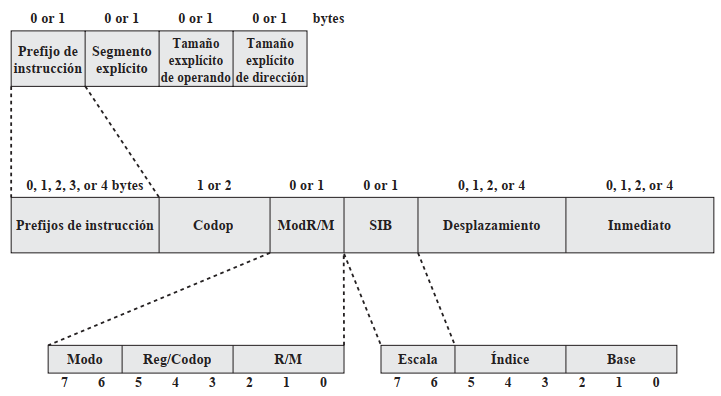
\includegraphics[width=1\linewidth]{images/formatoinstruccionx86} 

}

\caption{Formato de instrucciones del Pentium x86}\label{fig:FormatoInst}
\end{figure}

Un ejemplo típico de instrucción es:

\begin{lstlisting}
  ; Carga el valor inmediato 10 en el registro R0
  MOV AX, [BX+SI+16]
  \end{lstlisting}

Esta instrucción utiliza varios componentes, que el procesador debe decodificar antes de ejecutarla. Aunque esta flexibilidad es una ventaja en términos de funcionalidad, requiere técnicas avanzadas, como predicción de saltos y paralelización, para mantener la eficiencia en procesadores modernos \protect\hyperlink{ref-hennessy2017computer}{{[}13{]}}, \protect\hyperlink{ref-patterson_computer_2014}{{[}28{]}}.

\hypertarget{lenguaje-muxe1quina-y-lenguaje-ensamblador}{%
\section{Lenguaje máquina y lenguaje ensamblador}\label{lenguaje-muxe1quina-y-lenguaje-ensamblador}}

El lenguaje máquina es el conjunto de instrucciones que un procesador puede entender y ejecutar directamente. Cada procesador tiene su propio conjunto de instrucciones, que se representan en forma de números binarios. Estas instrucciones son específicas para cada arquitectura y están diseñadas para realizar operaciones básicas como sumar, restar, mover datos entre registros y acceder a la memoria. El lenguaje máquina es el nivel más bajo de programación y está compuesto por secuencias de bits que representan operaciones y operandos específicos del procesador
\protect\hyperlink{ref-hennessy2017computer}{{[}13{]}}, \protect\hyperlink{ref-irvine2011assembly}{{[}43{]}}.

El procesador ejecuta directamente las instrucciones codificadas en lenguaje máquina, sin requerir traducción desde niveles superiores de abstracción. Sin embargo, la escritura manual de código en lenguaje máquina es un proceso extremadamente laborioso, propenso a errores y difícil de mantener. Cada instrucción debe representarse como una cadena precisa de ceros y unos. Esta codificación depende de las reglas específicas del procesador, que incluyen los modos de direccionamiento, los formatos de instrucción y la organización de la memoria \protect\hyperlink{ref-stallings_computer_2021}{{[}14{]}}, \protect\hyperlink{ref-tanenbaum_structured_2016}{{[}22{]}}, \protect\hyperlink{ref-null_essentials_2014}{{[}27{]}}, \protect\hyperlink{ref-irvine2011assembly}{{[}43{]}}.

Por ejemplo, si un estudiante o desarrollador deseara sumar dos números en lenguaje máquina, tendría que especificar manualmente cada secuencia binaria correspondiente a la operación de suma, así como las direcciones de memoria donde se encuentran los operandos. Este enfoque no solo es tedioso, sino que también aumenta la probabilidad de errores, especialmente cuando se requiere modificar o depurar el código.

Ante las limitaciones del lenguaje máquina en términos de legibilidad y mantenibilidad, se desarrolló un lenguaje de bajo nivel con mayor legibilidad que el lenguaje máquina que permitiera al programador escribir instrucciones de forma más comprensible: el lenguaje ensamblador. Este lenguaje permite a los programadores escribir instrucciones más comprensibles mediante mnemónicos simbólicos, que actúan como representaciones legibles de las instrucciones en lenguaje máquina. Cada arquitectura de procesador define su propio conjunto de instrucciones (ISA, Instruction Set Architecture), lo que implica que el lenguaje ensamblador asociado debe ajustarse a la codificación binaria, modos de direccionamiento y sintaxis específicos de dicha ISA \protect\hyperlink{ref-stallings_computer_2021}{{[}14{]}}.

En el ámbito educativo, el lenguaje ensamblador se destaca como una herramienta fundamental para comprender cómo se comunican el software y el hardware \protect\hyperlink{ref-tanenbaum_structured_2016}{{[}22{]}}, \protect\hyperlink{ref-null_essentials_2014}{{[}27{]}}. Permite a los estudiantes visualizar la ejecución de instrucciones individuales, analizar el uso de registros y explorar la estructura de la memoria, convirtiéndose en un recurso valioso para este propósito.

Un programa en lenguaje ensamblador suele estar compuesto por instrucciones que especifican un mnemónico, uno o más operandos, y eventualmente el modo de direccionamiento. Por ejemplo:

\begin{lstlisting}
  ; Carga el valor inmediato 10 en el registro R0
  MOV AX, 5
  ADD AX, BX
  \end{lstlisting}

Estas líneas indican que el valor 5 se mueve al registro AX y luego se suma el contenido de BX. A través de este tipo de instrucciones, el estudiante puede visualizar de forma explícita cómo opera el procesador sobre sus registros y memoria.

\hypertarget{ensamblador}{%
\subsection{Ensamblador}\label{ensamblador}}

El ensamblador es un programa que traduce las instrucciones simbólicas escritas en lenguaje ensamblador a lenguaje máquina, es decir, las convierte en las secuencias binarias que el procesador puede interpretar y ejecutar. Este proceso de traducción es prácticamente directo, ya que existe una correspondencia uno a uno entre las instrucciones en ensamblador y las instrucciones en lenguaje máquina \protect\hyperlink{ref-stallings_computer_2021}{{[}14{]}}, \protect\hyperlink{ref-tanenbaum_structured_2016}{{[}22{]}}. En contraste, los lenguajes de programación de alto nivel, como C o Python, suelen generar múltiples instrucciones máquina por cada línea de código fuente, lo que los distancia más de la arquitectura subyacente \protect\hyperlink{ref-hennessy2017computer}{{[}13{]}}.

La Figura \ref{fig:ensambla} muestra el proceso de traducción de un programa en lenguaje ensamblador a lenguaje máquina. En este proceso, el ensamblador toma cada línea de código en ensamblador y la convierte en su representación binaria correspondiente, generando así un archivo ejecutable que puede ser cargado y ejecutado por el procesador.

\begin{figure}

{\centering 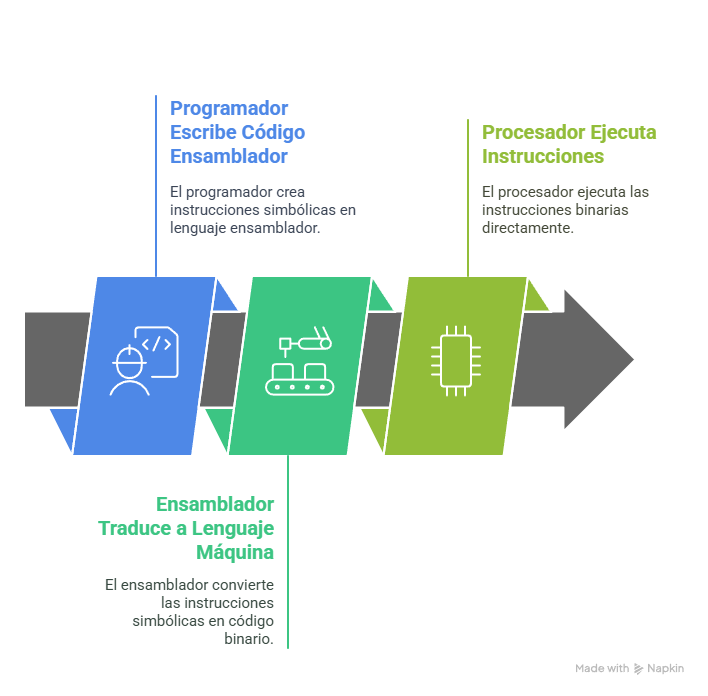
\includegraphics[width=1\linewidth]{images/ensamblador} 

}

\caption{Proceso de ensamblado}\label{fig:ensambla}
\end{figure}

\hypertarget{ensambladores-x86}{%
\subsection{Ensambladores x86}\label{ensambladores-x86}}

En el caso de la arquitectura x86, los programadores pueden elegir entre diversos ensambladores, como TASM (Turbo Assembler) \protect\hyperlink{ref-tasm}{{[}44{]}}, MASM (Microsoft Macro Assembler) \protect\hyperlink{ref-masm}{{[}45{]}} y NASM (Netwide Assembler) \protect\hyperlink{ref-nasm}{{[}46{]}}. Aunque cada ensamblador tiene características y sintaxis particulares, todos comparten el objetivo fundamental de convertir las instrucciones ensamblador en código binario ejecutable por los procesadores x86 \protect\hyperlink{ref-hyde2010art}{{[}47{]}}.

A continuación, se presenta una tabla comparativa \ref{tab:ensambladores} que resume las principales características de tres ensambladores ampliamente utilizados en la arquitectura x86. La información compilada permite visualizar diferencias relevantes en términos de sintaxis, compatibilidad, funcionalidades adicionales y contexto de uso, lo que resulta particularmente útil al momento de seleccionar herramientas adecuadas para entornos educativos o de desarrollo de bajo nivel.

\begin{table}[!h]
\centering
\caption{\label{tab:ensambladores}Comparación de ensambladores arquitectura x86}
\centering
\resizebox{\ifdim\width>\linewidth\linewidth\else\width\fi}{!}{
\fontsize{10}{12}\selectfont
\begin{tabular}[t]{>{\raggedright\arraybackslash}p{4cm}|>{\raggedright\arraybackslash}p{4cm}>{\raggedright\arraybackslash}p{4cm}>{\raggedright\arraybackslash}p{4cm}}
\toprule
\multicolumn{1}{>{\centering\arraybackslash}p{4cm}}{\cellcolor[HTML]{D3D3D3}{\textbf{Característica}}} & \multicolumn{1}{>{\centering\arraybackslash}p{4cm}}{\cellcolor[HTML]{D3D3D3}{\textbf{TASM}}} & \multicolumn{1}{>{\centering\arraybackslash}p{4cm}}{\cellcolor[HTML]{D3D3D3}{\textbf{MASM}}} & \multicolumn{1}{>{\centering\arraybackslash}p{4cm}}{\cellcolor[HTML]{D3D3D3}{\textbf{NASM}}}\\
\midrule
\textbf{Desarrollador} & Borland & Microsoft & Simon Tatham et al.\\
\addlinespace[10pt]
\textbf{Año de lanzamiento} & 1985 & 1981 & 1996\\
\addlinespace[10pt]
\textbf{Sistema operativo} & MS-DOS, Windows & MS-DOS, Windows & Multiplataforma (Windows, Linux, macOS)\\
\addlinespace[10pt]
\textbf{Sintaxis} & Sintaxis similar a Intel con extensiones & Sintaxis de Intel con soporte avanzado & Sintaxis de Intel, modular y extensible\\
\addlinespace[10pt]
\textbf{Soporte de macros} & Macros y directivas avanzadas & Macros y directivas extensivas & Macros avanzadas y preprocesamiento\\
\addlinespace[10pt]
\addlinespace
\textbf{Compatibilidad} & Compatibilidad con x86 antiguo & Compatibilidad con x86 antiguo & Compatibilidad con x86, x86-64 y otros\\
\addlinespace[10pt]
\textbf{Capacidades adicionales} & Integración con herramientas Borland & Integración con Visual Studio & Soporte para múltiples formatos (binario, ELF, etc.)\\
\addlinespace[10pt]
\textbf{Licencia} & Comercial & Comercial & Código abierto\\
\addlinespace[10pt]
\textbf{Uso actual} & Menos común, usado en entornos heredados & Ampliamente usado en desarrollo Windows & Popular en sistemas y software libre\\
\addlinespace[10pt]
\bottomrule
\end{tabular}}
\end{table}

\hypertarget{simulacion}{%
\chapter{Simulación}\label{simulacion}}

En este capítulo se analiza el papel de la simulación desde una perspectiva didáctica, destacando su relevancia como herramienta de apoyo en la enseñanza de Arquitectura de Computadoras. Se abordan los beneficios que ofrecen los simuladores en el proceso educativo y los desafíos que ayudan a superar en la formación de los estudiantes.

\hypertarget{introducciuxf3n-a-la-simulaciuxf3n}{%
\section{Introducción a la simulación}\label{introducciuxf3n-a-la-simulaciuxf3n}}

La simulación constituye una herramienta esencial en múltiples dominios, incluidos la medicina, la defensa, el entretenimiento y particularmente la educación, debido a su capacidad para representar procesos complejos y facilitar la toma de decisiones en entornos seguros y controlados. Su principal valor radica en su capacidad para modelar sistemas complejos, generar hipótesis, realizar análisis predictivos y explorar escenarios de manera segura y eficiente.

Banks define la simulación como el proceso de replicar el comportamiento de un sistema a lo largo del tiempo mediante un modelo conceptual que representa sus características y dinámicas principales \protect\hyperlink{ref-banks_discrete-event_2010}{{[}2{]}}. Estos modelos evolucionan simulando las interacciones entre sus componentes, lo que permite estudiar su respuesta ante diferentes variables y escenarios \protect\hyperlink{ref-robinson_simulation_2014}{{[}4{]}}.

La posibilidad de analizar sistemas complejos sin intervenir directamente en ellos convierte a la simulación en una herramienta indispensable en el contexto actual, marcado por el avance de la tecnología y la creciente complejidad de los sistemas. Además, la simulación permite optimizar diseños, prever comportamientos y reducir los costos de desarrollo antes de implementar soluciones reales \protect\hyperlink{ref-law_simulation_2015}{{[}3{]}}, \protect\hyperlink{ref-zeigler_theory_2000}{{[}20{]}}.

\hypertarget{aplicaciones-de-la-simulaciuxf3n-en-la-industria}{%
\subsection{Aplicaciones de la simulación en la industria}\label{aplicaciones-de-la-simulaciuxf3n-en-la-industria}}

En sectores como la industria automotriz, la simulación es fundamental para el diseño y prueba de sistemas de seguridad, como airbags y frenos. Gracias a modelos virtuales, se realizan pruebas de colisión y análisis de rendimiento sin necesidad de recurrir a costosas pruebas físicas. Asimismo, la simulación permite optimizar diseños de motores, analizar el flujo aerodinámico y prever el comportamiento de materiales en condiciones extremas, contribuyendo a mejorar tanto la eficiencia como la seguridad de los vehículos \protect\hyperlink{ref-stork_towards_2008}{{[}48{]}}.

En la aviación, los simuladores de vuelo son esenciales para entrenar pilotos, replicando condiciones reales de vuelo sin riesgos. Durante el diseño de aeronaves, estas herramientas permiten evaluar la aerodinámica y el rendimiento en diversos entornos, reduciendo significativamente el tiempo y los costos de desarrollo mientras incrementan la seguridad \protect\hyperlink{ref-jentsch_simulation_2017}{{[}49{]}}.

Estos principios generales encuentran aplicaciones concretas en diversos sectores industriales, donde la simulación cumple un papel clave tanto en el diseño como en el entrenamiento, la evaluación y la toma de decisiones.

\begin{table}[!h]
\centering
\caption{\label{tab:unnamed-chunk-2}Aplicaciones de la simulación en distintos sectores}
\centering
\resizebox{\ifdim\width>\linewidth\linewidth\else\width\fi}{!}{
\fontsize{10}{12}\selectfont
\begin{tabular}[t]{>{\raggedright\arraybackslash}p{4cm}|>{\raggedright\arraybackslash}p{4cm}>{\raggedright\arraybackslash}p{4cm}}
\toprule
\multicolumn{1}{>{\centering\arraybackslash}p{4cm}}{\cellcolor[HTML]{D3D3D3}{\textbf{Sector}}} & \multicolumn{1}{>{\centering\arraybackslash}p{4cm}}{\cellcolor[HTML]{D3D3D3}{\textbf{Aplicación}}} & \multicolumn{1}{>{\centering\arraybackslash}p{4cm}}{\cellcolor[HTML]{D3D3D3}{\textbf{Beneficio principal}}}\\
\midrule
\textbf{Automotriz} & Pruebas de colisión virtuales & Reducción de costos y aumento de seguridad\\
\addlinespace[10pt]
\textbf{Aeroespacial} & Simuladores de vuelo & Entrenamiento sin riesgo\\
\addlinespace[10pt]
\textbf{Medicina} & Simulación de cirugías & Entrenamiento sin comprometer pacientes\\
\addlinespace[10pt]
\textbf{Educación} & Simuladores para arquitectura de computadoras & Comprensión de procesos abstractos\\
\addlinespace[10pt]
\bottomrule
\end{tabular}}
\end{table}

Estos ejemplos ilustran cómo la simulación contribuye significativamente a la optimización de procesos, la reducción de riesgos y la mejora continua en el desarrollo de sistemas complejos. Su uso no solo ha transformado sectores productivos, sino que también ofrece un modelo replicable en contextos educativos especializados, como la enseñanza de arquitectura de computadoras.

\hypertarget{simulaciuxf3n-en-la-educaciuxf3n}{%
\section{Simulación en la educación}\label{simulaciuxf3n-en-la-educaciuxf3n}}

En contextos educativos, la simulación se ha consolidado como una estrategia pedagógica eficaz para facilitar la comprensión de fenómenos complejos, especialmente en disciplinas que requieren alto nivel de abstracción y razonamiento sistémico. A través de simuladores, los estudiantes pueden interactuar con sistemas virtuales y experimentar escenarios realistas, lo que mejora la comprensión de ideas abstractas y favorece la aplicación práctica de conocimientos teóricos \protect\hyperlink{ref-lion_simuladores_2005}{{[}5{]}}.

En contraste con enfoques instruccionales tradicionales centrados en la transmisión de información, los simuladores favorecen metodologías activas basadas en el aprendizaje por descubrimiento, la resolución de problemas y la construcción significativa del conocimiento, las herramientas de simulación integran tecnologías que vinculan conceptos teóricos con situaciones reales. Esto promueve una pedagogía interactiva, basada en la resolución de problemas y el aprendizaje por descubrimiento, estimulando la exploración y el razonamiento inferencial \protect\hyperlink{ref-contreras_uso_2010}{{[}6{]}}.

En definitiva, la simulación enriquece la experiencia de aprendizaje al proporcionar una plataforma dinámica y participativa que facilita tanto la experimentación como la asimilación profunda de los contenidos.

\hypertarget{el-rol-de-la-simulaciuxf3n-en-la-enseuxf1anza-de-arquitectura-de-computadoras}{%
\subsection{El rol de la simulación en la enseñanza de Arquitectura de Computadoras}\label{el-rol-de-la-simulaciuxf3n-en-la-enseuxf1anza-de-arquitectura-de-computadoras}}

En la carrera de Licenciatura en Sistemas, la asignatura Arquitectura de Computadoras persigue varios objetivos esenciales:
- Comprender la estructura y funcionamiento de las computadoras.
- Conocer las diferentes arquitecturas de sistemas microprocesadores.
- Evaluar medidas de rendimiento y comparar arquitecturas.
- Analizar el impacto de la tecnología de las computadoras en contextos sociales y económicos.

Enseñar los fundamentos teóricos de la organización y arquitectura interna de las computadoras puede ser un reto debido a la complejidad de los procesos involucrados. Los estudiantes necesitan desarrollar altos niveles de abstracción para construir modelos mentales que les permitan entender conceptos como la ejecución de instrucciones, la gestión de memoria o la interacción entre componentes del sistema.

En este contexto, los simuladores se configuran como mediadores didácticos que permiten representar gráficamente procesos abstractos, facilitando la manipulación de parámetros y el análisis de resultados en un entorno seguro, repetible y sin restricciones físicas. Estas herramientas permiten a los alumnos experimentar con configuraciones y parámetros, observar su impacto en el rendimiento del sistema y explorar escenarios hipotéticos sin necesidad de hardware físico.

Además, la simulación actúa como un puente entre la teoría y la práctica, facilitando que los docentes refuercen conceptos abstractos con experiencias concretas. En conjunto, estas ventajas hacen de la simulación una metodología pedagógica invaluable, promoviendo la experimentación y el aprendizaje activo en la enseñanza de Arquitectura de Computadoras \protect\hyperlink{ref-garcia-garcia_pbbcache_2020}{{[}7{]}}, \protect\hyperlink{ref-nova_tool_2013}{{[}8{]}}, \protect\hyperlink{ref-skrien_cpu_2001}{{[}18{]}}.

\hypertarget{el-formalismo-devs-discrete-event-system-specification}{%
\section{El Formalismo DEVS (Discrete Event System Specification)}\label{el-formalismo-devs-discrete-event-system-specification}}

El formalismo DEVS es una metodología modular y jerárquica que permite modelar y analizar sistemas representables como sistemas de eventos discretos, continuos o híbridos. Desarrollado por Bernard P. Zeigler en la década de 1970, este enfoque amplía el concepto de las máquinas de Moore al añadir una estructura que permite representar el comportamiento de sistemas mediante eventos temporizados que provocan cambios de estado, capturando así tanto la dinámica interna como las interacciones externas del sistema \protect\hyperlink{ref-zeigler_theory_2000}{{[}20{]}}.

\hypertarget{estructura-del-formalismo-devs}{%
\subsection{Estructura del formalismo DEVS}\label{estructura-del-formalismo-devs}}

Esta estructura permite capturar tanto el comportamiento interno como la interacción externa del sistema modelado.

DEVS describe el comportamiento de un sistema real utilizando eventos de entrada y salida, así como transiciones entre estados definidos. Un sistema en este formalismo se compone de dos tipos principales de modelos:

\begin{itemize}
\tightlist
\item
  \textbf{Modelos atómicos}: representan las unidades fundamentales de comportamiento.
\item
  \textbf{Modelos acoplados}: integran modelos atómicos y/o otros modelos acoplados, permitiendo la construcción jerárquica de sistemas más complejos.
\end{itemize}

Esta organización modular facilita el análisis y la gestión de sistemas, permitiendo probar subsistemas de manera aislada antes de integrarlos en un modelo completo.

La siguiente figura \ref{fig:devs} ilustra la organización modular del formalismo DEVS, mostrando cómo se integran modelos atómicos dentro de modelos acoplados:

\begin{figure}

{\centering 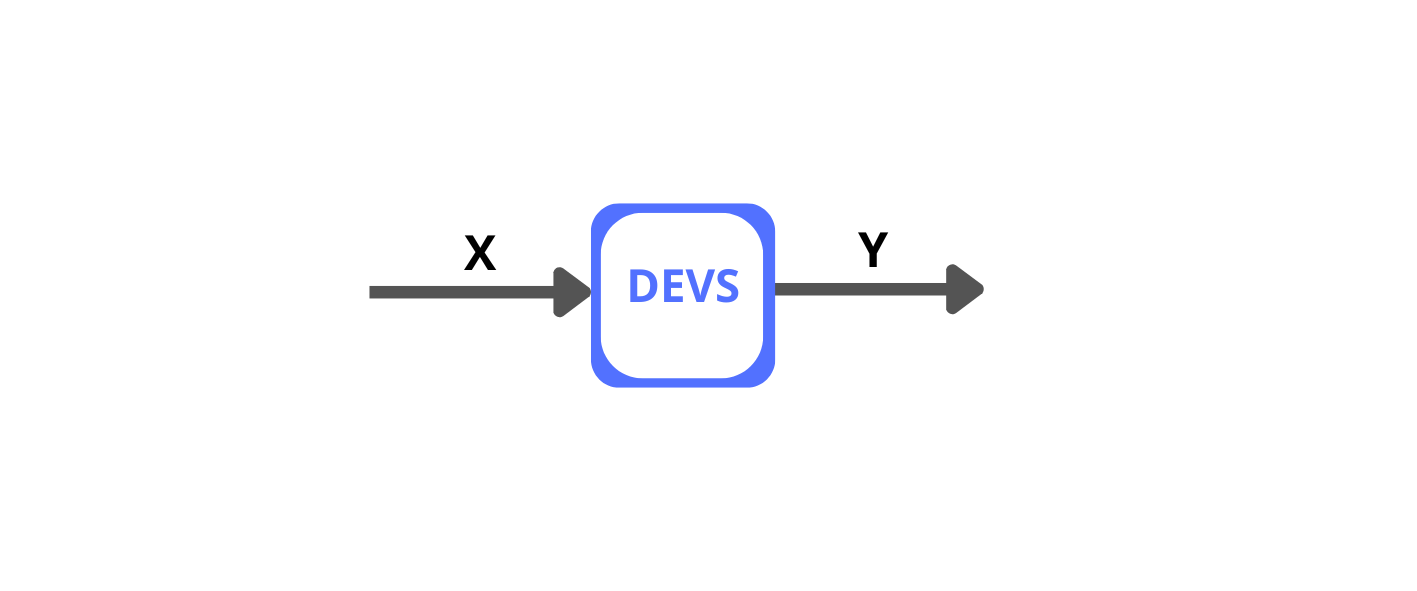
\includegraphics[width=1\linewidth]{images/devs} 

}

\caption{Relación entre modelos atómicos y modelos acoplados en DEVS}\label{fig:devs}
\end{figure}

\hypertarget{aplicaciones-del-formalismo-devs}{%
\subsection{Aplicaciones del formalismo DEVS}\label{aplicaciones-del-formalismo-devs}}

``El formalismo DEVS encuentra aplicación en diversos ámbitos, como las redes de comunicación \protect\hyperlink{ref-fujimoto2001parallel}{{[}50{]}}, donde permite simular el enrutamiento de paquetes y la congestión de redes; en entornos de manufactura \protect\hyperlink{ref-zeigler_theory_2000}{{[}20{]}}, donde se modelan flujos de producción y control de calidad; y en sistemas de transporte, para la optimización de flujos vehiculares \protect\hyperlink{ref-barros1997modeling}{{[}51{]}}. También se utiliza en la simulación de sistemas biológicos, como la propagación de enfermedades o el comportamiento de poblaciones \protect\hyperlink{ref-zeigler2004continuity}{{[}52{]}}. En el ámbito de la educación, DEVS se ha implementado en simuladores para la enseñanza de arquitectura de computadoras, permitiendo a los estudiantes explorar y comprender conceptos complejos mediante la visualización y manipulación de modelos \protect\hyperlink{ref-calvo2010simulador}{{[}53{]}}.

Estas aplicaciones destacan su versatilidad para optimizar sistemas complejos en escenarios del mundo real.

\hypertarget{devs-en-la-enseuxf1anza-de-la-arquitectura-de-computadoras}{%
\subsection{DEVS en la enseñanza de la Arquitectura de Computadoras}\label{devs-en-la-enseuxf1anza-de-la-arquitectura-de-computadoras}}

La implementación de entornos de simulación basados en DEVS en la enseñanza de arquitectura de computadoras aporta múltiples ventajas que enriquecen el proceso de aprendizaje:

\begin{itemize}
\tightlist
\item
  \textbf{Representación visual}: ofrece diagramas y representaciones dinámicas que ayudan a los estudiantes a visualizar y comprender procesos internos, como la ejecución de instrucciones y la gestión de recursos.
\item
  \textbf{Interactividad}: permite modificar configuraciones y parámetros, fomentando la experimentación y mostrando el impacto directo de estas variables en el rendimiento del sistema.
\item
  \textbf{Exploración de escenarios}: posibilita simular escenarios hipotéticos y evaluar el comportamiento de sistemas complejos sin la necesidad de hardware físico.
\end{itemize}

Estas funcionalidades enriquecen la experiencia educativa al integrar la teoría con la práctica y fomentar una participación activa en el análisis de los principios fundamentales de la arquitectura computacional. Al adoptar DEVS como parte del entorno educativo, se potencia la capacidad de los estudiantes para abordar problemas complejos y explorar soluciones innovadoras \protect\hyperlink{ref-calvo_valdes_simulador_2010}{{[}54{]}}.

En conclusión, el formalismo DEVS no solo es una herramienta valiosa para el modelado y análisis de sistemas, sino que también representa un recurso poderoso para facilitar la enseñanza de conceptos complejos, como los que se encuentran en la arquitectura de computadoras.

\hypertarget{comparativa}{%
\chapter{Comparativa de simuladores}\label{comparativa}}

Este capítulo presenta un análisis comparativo de simuladores basados en la arquitectura x86, con el objetivo de determinar su adecuación para su integración en la asignatura Arquitectura de Computadoras de la Licenciatura en Sistemas de Información.

La selección y evaluación de estos simuladores se fundamenta en criterios específicos diseñados para medir su efectividad en un entorno educativo. El objetivo principal es identificar las herramientas que mejor respalden el proceso de enseñanza y aprendizaje. Los criterios definidos abarcan aspectos clave para la enseñanza de arquitectura de computadoras: facilidad de uso, funcionalidades del entorno de programación, calidad de los recursos de apoyo, mecanismos de ejecución de programas, precisión en la emulación de la arquitectura x86, características técnicas del software y su alineación con los contenidos curriculares.

Los resultados de esta investigación fueron publicados en el XVII Congreso de Tecnología en Educación y Educación en Tecnología (2022), en el trabajo titulado Herramientas de software para dar soporte en la enseñanza y aprendizaje de la arquitectura x86 \protect\hyperlink{ref-colombani_herramientas_2022}{{[}55{]}}.

\hypertarget{estudios-similares}{%
\section{Estudios similares}\label{estudios-similares}}

Existen antecedentes de estudios comparativos que evalúan simuladores aplicados a la enseñanza en cursos de arquitectura de computadoras:
- ``A survey and evaluation of simulators suitable for teaching courses in computer architecture and organization'', 2009 \protect\hyperlink{ref-nikolic_survey_2009}{{[}11{]}}: este estudio analiza simuladores considerando dos categorías principales. La primera, relacionada con las características de simulación, incluye criterios como granularidad, usabilidad, disponibilidad, presentación visual y flujo de simulación. La segunda categoría evalúa la cobertura de los contenidos establecidos en los planes de estudio.
- ``Survey and evaluation of simulators suitable for teaching for computer architecture and organization Supporting undergraduate students at Sir Syed University of Engineering \& Technology'', 2012 \protect\hyperlink{ref-hasan_survey_2012}{{[}12{]}}: este trabajo evalúa aspectos como la usabilidad, disponibilidad, fundamentos de arquitectura informática, jerarquía de sistemas de memoria, comunicación e interfaz, y diseño de sistemas de procesadores.

A diferencia de los estudios mencionados, este trabajo propone una evaluación centrada exclusivamente en simuladores de arquitectura x86, mediante el uso de criterios diseñados ad hoc para analizar tanto las funcionalidades de simulación como su adecuación a los contenidos específicos de la asignatura Arquitectura de Computadoras dictada en la Licenciatura en Sistemas de la Universidad Nacional de Entre Ríos.

\hypertarget{simuladores-bajo-anuxe1lisis}{%
\section{Simuladores bajo análisis}\label{simuladores-bajo-anuxe1lisis}}

Un simulador de arquitectura es una herramienta de software que emula el hardware de un sistema de cómputo, permitiendo representar aspectos arquitectónicos y funcionales del mismo. Estos simuladores ofrecen un entorno controlado para realizar pruebas, modificaciones y ejecución de programas sin riesgo de dañar componentes físicos o enfrentar limitaciones de hardware \protect\hyperlink{ref-radivojevic_design_2011}{{[}10{]}}.

Algunos simuladores destacan por proporcionar una representación visual e interactiva de la organización y arquitectura interna de una computadora, facilitando la comprensión de su funcionamiento. Algunos ejemplos relevantes de simuladores son: Assembly Debugger (x86), Simple 8-bit Assembler Simulator, Microprocessor Simulator, Simulador de ensamblador de 16 bits y Emu8086. Estas herramientas juegan un papel fundamental en el aprendizaje de la arquitectura de computadoras, al conectar conceptos teóricos con experiencias prácticas y simplificar abstracciones complejas, además de servir como soporte en la labor docente \protect\hyperlink{ref-nikolic_survey_2009}{{[}11{]}}, \protect\hyperlink{ref-hasan_survey_2012}{{[}12{]}}, \protect\hyperlink{ref-hennessy2017computer}{{[}13{]}}, \protect\hyperlink{ref-stallings_computer_2021}{{[}14{]}}, \protect\hyperlink{ref-behrooz_computer_2005}{{[}56{]}}.

\hypertarget{criterios-de-evaluaciuxf3n}{%
\section{Criterios de evaluación}\label{criterios-de-evaluaciuxf3n}}

Los criterios de evaluación se definieron con el objetivo de realizar un análisis integral y sistemático de los simuladores seleccionados. A continuación, se presentan estos criterios junto con sus respectivos indicadores y escalas:

\begin{itemize}
\tightlist
\item
  \textbf{Usabilidad}: evalúa la facilidad de uso del simulador.

  \begin{itemize}
  \tightlist
  \item
    \textbf{Indicadores}:

    \begin{itemize}
    \tightlist
    \item
      Facilidad de aprendizaje (tiempo necesario para familiarizarse con la herramienta).
    \item
      Interfaz de usuario (claridad y organización).
    \item
      Documentación y ayuda (accesibilidad y calidad de tutoriales y guías).
    \end{itemize}
  \item
    \textbf{Escala}: Difícil - Media - Fácil.
  \end{itemize}
\item
  \textbf{Editor}: analiza las funcionalidades para escribir y depurar código ensamblador.

  \begin{itemize}
  \tightlist
  \item
    \textbf{Indicadores}:

    \begin{itemize}
    \tightlist
    \item
      Capacidad de edición (resaltado de sintaxis, puntos de interrupción, etc.).
    \item
      Manejo de errores de sintaxis.
    \item
      Opciones de almacenamiento (guardar y cargar programas).
    \end{itemize}
  \item
    \textbf{Escala}: Baja - Media - Alta.
  \end{itemize}
\item
  \textbf{Documentación}: valora la disponibilidad y calidad de los recursos de aprendizaje proporcionados.

  \begin{itemize}
  \tightlist
  \item
    \textbf{Indicadores}:

    \begin{itemize}
    \tightlist
    \item
      Manual de usuario.
    \item
      Tutoriales de aprendizaje.
    \item
      Exhaustividad en la descripción del repertorio de instrucciones.
    \end{itemize}
  \item
    \textbf{Escala}: Mínima - Media - Completa.
  \end{itemize}
\item
  \textbf{Ejecución de simulación}: mide la facilidad para controlar y observar la ejecución de programas.

  \begin{itemize}
  \tightlist
  \item
    \textbf{Indicadores}:

    \begin{itemize}
    \tightlist
    \item
      Control de simulación (pausa, reanudación, retroceso).
    \item
      Visualización del flujo de ejecución.
    \item
      Configurabilidad (ajuste de parámetros como la velocidad del reloj).
    \end{itemize}
  \item
    \textbf{Escala}: Baja - Media - Alta.
  \end{itemize}
\item
  \textbf{Nivel de especificación de la Organización y Arquitectura del sistema simulado}: determina la precisión en la representación de la arquitectura x86.

  \begin{itemize}
  \tightlist
  \item
    \textbf{Indicadores}:

    \begin{itemize}
    \tightlist
    \item
      Fidelidad en la representación de la arquitectura.
    \item
      Completitud del conjunto de instrucciones implementadas.
    \item
      Inclusión y funcionalidad de memoria y módulos de E/S.
    \end{itemize}
  \item
    \textbf{Escala}: Mínima - Media - Completa.
  \end{itemize}
\item
  \textbf{Características del producto software}: evalúa las propiedades generales del simulador.

  \begin{itemize}
  \tightlist
  \item
    \textbf{Indicadores}:

    \begin{itemize}
    \tightlist
    \item
      Tipo de licencia (open source o privativa).
    \item
      Frecuencia de actualizaciones.
    \item
      Plataforma (aplicación web o de escritorio)
    \end{itemize}
  \item
    \textbf{Escala}: Mala - Buena - Muy buena.
  \end{itemize}
\item
  \textbf{Cobertura de los contenidos preestablecidos en la currícula}: mide el grado en que el simulador abarca los contenidos de la asignatura.

  \begin{itemize}
  \tightlist
  \item
    \textbf{Indicadores}:

    \begin{itemize}
    \tightlist
    \item
      Alineación con los tópicos del currículum.
    \item
      Profundidad en el tratamiento de los temas.
    \end{itemize}
  \item
    \textbf{Escala}: Baja - Media - Alta.
  \end{itemize}
\end{itemize}

La Tabla \ref{tab:criterios} resume los criterios, indicadores y escalas utilizadas.

\begin{table}[!h]
\centering
\caption{\label{tab:criterios}Criterios e indicadores de evaluación de simuladores}
\centering
\resizebox{\ifdim\width>\linewidth\linewidth\else\width\fi}{!}{
\begin{tabular}[t]{>{\raggedright\arraybackslash}p{4cm}|>{\raggedright\arraybackslash}p{5cm}>{\raggedright\arraybackslash}p{5cm}}
\toprule
\multicolumn{1}{>{\centering\arraybackslash}p{4cm}}{\cellcolor[HTML]{D3D3D3}{\textbf{Criterio}}} & \multicolumn{1}{>{\centering\arraybackslash}p{5cm}}{\cellcolor[HTML]{D3D3D3}{\textbf{Indicadores}}} & \multicolumn{1}{>{\centering\arraybackslash}p{5cm}}{\cellcolor[HTML]{D3D3D3}{\textbf{Escala}}}\\
\midrule
\textbf{Usabilidad} & Facilidad de aprendizaje, interfaz, documentación & Difícil - Fácil\\
\textbf{Funcionalidad del editor} & Sintaxis, manejo de errores, guardar/cargar & Baja - Alta\\
\textbf{Calidad de la documentación} & Manuales, tutoriales, repertorio de instrucciones & Mínima - Completa\\
\textbf{Ejecución de simulación} & Control de simulación, visualización del flujo, configurabilidad & Baja - Alta\\
\textbf{Especificación de arquitectura x86} & Fidelidad de la arquitectura, repertorio, memoria y E/S & Mínima - Completa\\
\addlinespace
\textbf{Propiedades técnicas y de distribución} & Licencia, actualizaciones, plataforma & Mala - Muy buena\\
\textbf{Alineación con contenidos curriculares} & Cobertura de tópicos, profundidad del tratamiento & Baja - Alta\\
\bottomrule
\end{tabular}}
\end{table}

\hypertarget{selecciuxf3n-de-simuladores}{%
\section{Selección de simuladores}\label{selecciuxf3n-de-simuladores}}

Mediante una exploración exhaustiva de fuentes disponibles en línea, foros académicos y repositorios educativos, se identificaron los siguientes simuladores de arquitectura x86: Assembly Debugger (x86), Simple 8-bit Assembler Simulator, Microprocessor Simulator, Simulador de ensamblador de 16 bits, Emu8086, VonSim, Orga1 y Qsim. Estos simuladores fueron seleccionados por su relevancia en el ámbito educativo y su potencial para facilitar la enseñanza de la arquitectura x86.

La selección se basó en una evaluación preliminar que consideró el tiempo necesario para su análisis y el grado de cumplimiento de los criterios definidos, priorizando aquellos simuladores que ofrecieran un balance adecuado entre funcionalidad, usabilidad, documentación y alineación con los contenidos curriculares de la asignatura Arquitectura de Computadoras. De esta preselección, se eligieron tres herramientas que, a priori, cumplían con la mayor cantidad de criterios evaluativos: \textbf{Emu8086}, \textbf{VonSim} y \textbf{Simple 8-bit Assembler Simulator}.

\begin{table}[!h]
\centering
\caption{\label{tab:simuladores}Proceso de selección de simuladores}
\centering
\resizebox{\ifdim\width>\linewidth\linewidth\else\width\fi}{!}{
\begin{tabular}[t]{>{}l|>{\raggedright\arraybackslash}p{4cm}>{\raggedright\arraybackslash}p{4cm}}
\toprule
\multicolumn{1}{c}{\cellcolor[HTML]{D3D3D3}{\textbf{Simulador}}} & \multicolumn{1}{>{\centering\arraybackslash}p{4cm}}{\cellcolor[HTML]{D3D3D3}{\textbf{Exploración.Previa}}} & \multicolumn{1}{>{\centering\arraybackslash}p{4cm}}{\cellcolor[HTML]{D3D3D3}{\textbf{Evaluación.Final}}}\\
\midrule
\textbf{Assembly Debugger (x86)} & 1 & 0\\
\textbf{Simple 8-bit Assembler Simulator} & 1 & 1\\
\textbf{Microprocessor Simulator} & 1 & 0\\
\textbf{Simulador de ensamblador de 16 bits} & 1 & 0\\
\textbf{Emu8086} & 1 & 1\\
\addlinespace
\textbf{VonSim} & 1 & 1\\
\textbf{Orga1} & 1 & 0\\
\textbf{Qsim} & 1 & 0\\
\bottomrule
\end{tabular}}
\end{table}

\hypertarget{participantes-en-la-evaluaciuxf3n}{%
\section{Participantes en la evaluación}\label{participantes-en-la-evaluaciuxf3n}}

La evaluación fue llevada a cabo por un equipo conformado por tres docentes de la asignatura Arquitectura de Computadoras ---Marcelo A. Colombani, José M. Ruiz y Amalia G. Delduca---, quienes aportaron su experiencia en el uso pedagógico de simuladores. Asimismo, se contó con la participación de un asesor externo, Marcelo A. Falappa, quien aportó una perspectiva independiente y validó tanto la metodología como los resultados obtenidos.

\hypertarget{anuxe1lisis-comparativo}{%
\section{Análisis comparativo}\label{anuxe1lisis-comparativo}}

A continuación, se presenta un análisis detallado de los simuladores seleccionados, basado en los criterios previamente establecidos:

\hypertarget{simple-8-bit-assembler-simulator}{%
\subsection{Simple 8-bit Assembler Simulator}\label{simple-8-bit-assembler-simulator}}

\begin{itemize}
\tightlist
\item
  \textbf{Usabilidad}: Nivel medio. Todos los componentes se muestran en una sola pantalla, lo que puede resultar abrumador para usuarios principiantes.
\item
  \textbf{Editor}: Nivel bajo. Incluye notificaciones de errores de sintaxis al ensamblar, pero carece de resaltado de sintaxis, puntos de interrupción (breakpoints) y opciones para guardar o cargar programas.
\item
  \textbf{Documentación}: Nivel mínimo. Consta solo de un manual de instrucciones implementadas.
\item
  \textbf{Ejecución de simulación}: Nivel medio. Permite ajustar la velocidad del reloj de la CPU y proporciona controles básicos de simulación.
\item
  \textbf{Nivel de especificación}: Nivel mínimo. Simplifica la arquitectura x86 a un CPU de 8 bits con 256 bytes de memoria y sin soporte para operaciones de entrada/salida (IN/OUT).
\item
  \textbf{Desarrollo del producto}: Nivel bueno. Licencia MIT, última actualización en 2015, desarrollado como una plataforma web.
\item
  \textbf{Cobertura de contenidos}: Nivel bajo. No incluye memoria independiente para módulos de entrada y salida, rutinas de interrupciones ni representación visual del ciclo de instrucción.
\end{itemize}

\hypertarget{vonsim}{%
\subsection{VonSim}\label{vonsim}}

\begin{itemize}
\tightlist
\item
  \textbf{Usabilidad}: Nivel medio. Utiliza solapas para presentar los componentes, lo que puede ser confuso para usuarios iniciales.
\item
  \textbf{Editor}: Nivel medio. Proporciona notificaciones de errores de sintaxis, resaltado de código y puntos de interrupción mediante software.
\item
  \textbf{Documentación}: Nivel medio. Incluye un manual de uso y un tutorial interactivo.
\item
  \textbf{Ejecución de simulación}: Nivel medio. Permite ajustar la velocidad del reloj de la CPU y ofrece controles básicos de simulación.
\item
  \textbf{Nivel de especificación}: Nivel medio. Representa una simplificación del procesador 8088 con arquitectura de 16 bits y memoria direccionable de 16 KiB.
\item
  \textbf{Desarrollo del producto}: Nivel muy bueno. Licencia GNU Affero General Public License v3.0, última versión en 2020, con amplia evidencia de uso académico.
\item
  \textbf{Cobertura de contenidos}: Nivel medio. Implementa dispositivos internos y externos, pero carece de visualización del ciclo de instrucción y métricas de rendimiento.
\end{itemize}

\hypertarget{emu8086}{%
\subsection{Emu8086}\label{emu8086}}

\begin{itemize}
\tightlist
\item
  \textbf{Usabilidad}: Nivel fácil. Inicialmente muestra el editor y permite activar los componentes del simulador a medida que se cargan programas.
\item
  \textbf{Editor}: Nivel alto. Incluye notificaciones de errores de sintaxis, resaltado de código, puntos de interrupción y opciones para guardar/cargar programas.
\item
  \textbf{Documentación}: Nivel completo. Ofrece un manual de instrucciones con ejemplos, un tutorial de aprendizaje y una guía de uso detallada.
\item
  \textbf{Ejecución de simulación}: Nivel alto. Proporciona control avanzado de la simulación, como retroceder una instrucción (``step back'').
\item
  \textbf{Nivel de especificación}: Nivel completo. Detalla la arquitectura del procesador 8086, con memoria direccionable de 1 MiB y soporte para interrupciones de software y hardware.
\item
  \textbf{Desarrollo del producto}: Nivel bueno. Licencia privativa, última actualización en 2023, desarrollado para plataformas de escritorio.
\item
  \textbf{Cobertura de contenidos}: Nivel alto. Emula el arranque (bootstrapping) de una IBM PC desde un disco flexible (floppy disk) y soporta todos los modos de direccionamiento.
\end{itemize}

\begin{longtable}[]{@{}llll@{}}
\caption{\label{tab:tabla-comparativa-criterios}Comparativa según criterios de evaluación preestablecidos}\tabularnewline
\toprule\noalign{}
Criterio.de.Evaluación & Simple.8.bit & VonSim & Emu8086 \\
\midrule\noalign{}
\endfirsthead
\toprule\noalign{}
Criterio.de.Evaluación & Simple.8.bit & VonSim & Emu8086 \\
\midrule\noalign{}
\endhead
\bottomrule\noalign{}
\endlastfoot
Usabilidad & Medio & Medio & Fácil \\
Editor & Bajo & Medio & Alto \\
Documentación & Mínima & Media & Completa \\
Ejecución de simulación & Medio & Medio & Alta \\
Nivel de especificación x86 & Mínima & Media & Completa \\
Características del producto & Buena & Muy buena & Buena \\
Cobertura de contenidos & Baja & Media & Alta \\
\end{longtable}

\hypertarget{resultados}{%
\section{Resultados}\label{resultados}}

La asignatura promueve el uso de simuladores para apoyar la enseñanza y el aprendizaje, permitiendo aplicar los contenidos desarrollados en máquinas reales. Emu8086 es la herramienta más adecuada para esta finalidad, ya que facilita la implementación de programas en hardware real. Sin embargo, su dependencia de MS-DOS complica su ejecución en sistemas operativos actuales, requiriendo el uso de emuladores de MS-DOS, lo que añade complejidad al proceso de enseñanza y aprendizaje.

Desde 2018, la asignatura utiliza la versión 4.08 de Emu8086. La herramienta tiene un periodo de evaluación gratuito de 14 días, después del cual se debe adquirir una licencia. Esto es un inconveniente, ya que se busca que los estudiantes puedan acceder a las herramientas de forma libre y gratuita.

Utilizar lenguaje NASM (Netwide Assembler) garantiza soporte tanto para Linux como Windows a través de herramientas libres como GCC (GNU Compiler Collection), generando programas para la arquitectura x86 de 16, 32 y 64 bits.

Emu8086 destaca por su interfaz dinámica, que muestra componentes como la pila, flags, teclado y pantalla solo cuando son necesarios, a diferencia de otros simuladores que presentan todos sus componentes desde el inicio.

Emu8086 sobresale particularmente en los aspectos vinculados a la edición, documentación y control de la ejecución. Su editor permite establecer puntos de ruptura, retroceder una instrucción, y guardar o recuperar programas desde la interfaz. Además, ofrece una documentación extensa, que incluye un repertorio de instrucciones con ejemplos, un tutorial para el aprendizaje del lenguaje ensamblador y un manual detallado del entorno de desarrollo. Estas características lo posicionan como una herramienta completa en términos de acompañamiento a los procesos de enseñanza y aprendizaje.

En el criterio de evaluación cuatro, Emu8086 se destaca por ofrecer una mayor cantidad de controladores para gestionar el flujo de ejecución, como la capacidad de retroceder la ejecución de una instrucción y recargar el programa actual.

En cuanto al nivel de especificación, Emu8086 representa con gran precisión la arquitectura x86, incluyendo soporte para interrupciones del sistema operativo MS-DOS. Esta característica permite simular de manera realista programas que podrían ejecutarse en un entorno compatible, constituyendo una ventaja significativa frente a los otros simuladores analizados.

En el criterio de evaluación seis VonSim se destaca del resto debido a que es licencia libre y posee una comunidad que respalda el proyecto.

En cuanto al último criterio, ninguna de las herramientas evaluadas cubre todos los contenidos que se pretende desarrollar con la ayuda de una herramienta, quedando excluido pasos del ciclo de instrucción y medidas de rendimientos (tiempo de CPU y CPI: ciclo por instrucción).

A partir del análisis comparativo, se destacan las siguientes observaciones clave:

\begin{itemize}
\tightlist
\item
  \textbf{Emu8086} presenta la interfaz más intuitiva y completa, con amplia documentación y una simulación precisa de la arquitectura x86. Sin embargo, su licencia privativa y la necesidad de emuladores para su ejecución en sistemas actuales constituyen limitaciones relevantes.
\item
  \textbf{VonSim}, con su licencia libre y actualización reciente, representa una alternativa interesante desde una perspectiva de software abierto, aunque su cobertura de contenidos y nivel de especificación son limitados en comparación.
\item
  \textbf{Simple 8-bit Assembler Simulator} resulta insuficiente para cubrir los objetivos curriculares de la asignatura, debido a su bajo nivel de complejidad, escasa documentación y capacidades limitadas de simulación.
\end{itemize}

En conclusión, si bien cada simulador ofrece ventajas puntuales, ninguno logra satisfacer plenamente los requerimientos pedagógicos y técnicos de la asignatura en su totalidad. Por ello, se recomienda continuar utilizando Emu8086 de manera transitoria, mientras se avanza en el desarrollo de un simulador propio que integre sus fortalezas, opere con licencia libre y sea compatible con entornos modernos. Esta iniciativa permitirá una mayor adecuación curricular, accesibilidad tecnológica y sostenibilidad en el tiempo.

\hypertarget{publicaciuxf3n}{%
\subsection{Publicación}\label{publicaciuxf3n}}

Este análisis comparativo fue publicado en el XVII Congreso de Tecnología en Educación y Educación en Tecnología (2022), bajo el título ``Herramientas de software para dar soporte en la enseñanza y aprendizaje de la arquitectura x86''\protect\hyperlink{ref-colombani_herramientas_2022}{{[}55{]}}.

Además, durante este proceso se estableció contacto con un desarrollador de VonSim, logrando implementar mejoras significativas, como animaciones de ejecución y documentación en línea, disponibles en su última versión publicada en agosto de 2023.

\hypertarget{desarrollo}{%
\chapter{Diseño y Construcción del Simulador}\label{desarrollo}}

En este capítulo se describe el diseño y desarrollo de una herramienta de simulación específica para la arquitectura x86, orientada a facilitar la enseñanza de los principios de arquitectura de computadoras. Se detalla la justificación del diseño, los pasos seguidos para su construcción y los métodos utilizados para validar su funcionalidad.

En el capítulo anterior se analizaron y evaluaron las herramientas de simulación existentes para la arquitectura x86. Esta revisión exhaustiva permitió identificar las limitaciones de las soluciones actuales y fundamentar la necesidad de desarrollar una herramienta específica, cuyos resultados fueron publicados posteriormente.

Para cumplir con este objetivo, el diseño de la herramienta sigue una serie de requisitos establecidos que guían su desarrollo, validación y alineación con los objetivos pedagógicos.

\hypertarget{requisitos-de-la-herramienta}{%
\section{Requisitos de la herramienta}\label{requisitos-de-la-herramienta}}

La herramienta de simulación está diseñada para cumplir los siguientes requisitos:

\begin{enumerate}
\def\labelenumi{\arabic{enumi}.}
\tightlist
\item
  \textbf{Representación global de la estructura y funcionamiento de la computadora:}

  \begin{itemize}
  \tightlist
  \item
    Representar de forma gráfica la arquitectura general de la computadora (CPU, bus, memoria y dispositivos de E/S) durante la ejecución de programas, destacando los componentes relevantes en cada etapa del proceso.
  \end{itemize}
\item
  \textbf{Soporte para la generación y ejecución de programas en ensamblador:}

  \begin{itemize}
  \tightlist
  \item
    Permitir tanto la ejecución paso a paso como la ejecución completa de programas en lenguaje ensamblador, promoviendo la comprensión detallada de cada instrucción.
  \end{itemize}
\item
  \textbf{Repertorio de instrucciones reducido y habilitación progresiva:}

  \begin{itemize}
  \tightlist
  \item
    Seleccionar un subconjunto esencial de instrucciones x86, que se habiliten progresivamente según avance la asignatura, adaptándose al ritmo de aprendizaje de los estudiantes. Esta estrategia didáctica facilita la asimilación gradual del conjunto de instrucciones (ISA) y es consistente con enfoques pedagógicos en el área de organización y arquitectura de computadores \protect\hyperlink{ref-null2018essentials}{\textbf{null2018essentials?}}, \protect\hyperlink{ref-stallings2021computer}{\textbf{stallings2021computer?}}.
  \end{itemize}
\item
  \textbf{Simulación visual e interactiva de micropasos de instrucciones:}

  \begin{itemize}
  \tightlist
  \item
    Representar el flujo de datos con el lenguaje de transferencia entre registros (RTL), destacando visualmente cada componente involucrado en la ejecución de un programa.
  \end{itemize}
\item
  \textbf{Gestión básica de interrupciones y periféricos:}

  \begin{itemize}
  \tightlist
  \item
    Incorporar un vector de interrupción predefinido para interactuar con dispositivos como teclado y monitor. También incluir instrucciones IN y OUT, junto con un módulo simplificado de entrada/salida.
  \end{itemize}
\item
  \textbf{Métricas de rendimiento:}

  \begin{itemize}
  \tightlist
  \item
    Proporcionar indicadores clave como tiempo de ciclo, tiempo de CPU y ciclos por instrucción (CPI) para analizar la ejecución de programas. Según Hennessy y Patterson \protect\hyperlink{ref-hennessy2017computer}{{[}13{]}}, estos indicadores permiten evaluar la eficiencia del procesamiento a nivel de arquitectura.
  \end{itemize}
\end{enumerate}

\hypertarget{diseuxf1o-conceptual}{%
\section{Diseño conceptual}\label{diseuxf1o-conceptual}}

Una vez establecidos los requisitos funcionales y pedagógicos de la herramienta, se procede a detallar su diseño conceptual, el cual traduce dichos lineamientos en una arquitectura concreta del simulador. Esta planificación garantiza la coherencia entre el diseño técnico y los objetivos de enseñanza propuestos.

La Figura \ref{fig:esquemavonsim8} representa la arquitectura general del simulador. Esta representación visual permite distinguir los flujos diferenciados de control e información durante la ejecución de los programas, facilitando la comprensión de la segmentación funcional del sistema simulado.

\begin{figure}

{\centering 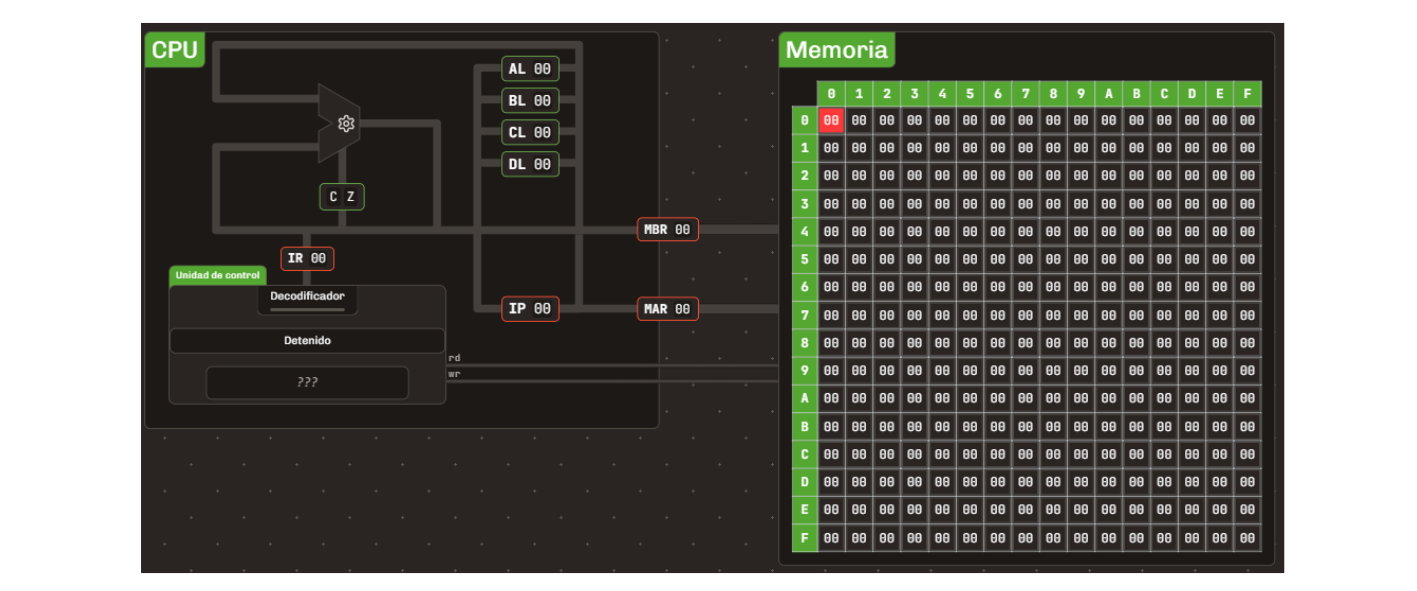
\includegraphics[width=0.85\linewidth]{images/esquemavonsim8} 

}

\caption{Arquitectura general del simulador}\label{fig:esquemavonsim8}
\end{figure}

\hypertarget{modelo-arquitectuxf3nico}{%
\subsection{Modelo arquitectónico}\label{modelo-arquitectuxf3nico}}

Se propone una versión simplificada de \textbf{8 bits} basada en la arquitectura \textbf{x86}, diseñada con un repertorio de instrucciones reducido y un conjunto de componentes esenciales. La elección de una arquitectura de 8 bits responde a una estrategia didáctica: al reducir la complejidad del sistema original, se prioriza la comprensión conceptual sobre la fidelidad técnica, conservando la esencia del repertorio x86.

\hypertarget{principales-bloques-funcionales}{%
\subsubsection{Principales bloques funcionales}\label{principales-bloques-funcionales}}

El simulador se compone de los siguientes bloques funcionales:

\begin{table}[!h]
\centering
\caption{\label{tab:bloquesfuncionales}Bloques funcionales principales}
\centering
\resizebox{\ifdim\width>\linewidth\linewidth\else\width\fi}{!}{
\fontsize{10}{12}\selectfont
\begin{tabular}[t]{>{\raggedright\arraybackslash}p{6cm}|>{\raggedright\arraybackslash}p{9cm}}
\toprule
\multicolumn{1}{>{\centering\arraybackslash}p{6cm}}{\cellcolor[HTML]{D3D3D3}{\textbf{Bloque Funcional}}} & \multicolumn{1}{>{\centering\arraybackslash}p{9cm}}{\cellcolor[HTML]{D3D3D3}{\textbf{Descripción}}}\\
\midrule
\textbf{Unidad Central de Procesamiento (CPU)} & Simulación de registros, Unidad de Control (UC) y Unidad Aritmética y Lógica (ALU).\\
\addlinespace[10pt]
\textbf{Memoria} & Estructura de memoria y simulación de operaciones de lectura y escritura.\\
\addlinespace[10pt]
\textbf{Sistema de Entrada/Salida (E/S)} & Interacción con periféricos y manejo de interrupciones.\\
\addlinespace[10pt]
\textbf{Bus de datos, direcciones y control} & Modelado de la comunicación entre componentes.\\
\addlinespace[10pt]
\bottomrule
\end{tabular}}
\end{table}

\hypertarget{caracteruxedsticas-del-cpu}{%
\subsubsection{Características del CPU}\label{caracteruxedsticas-del-cpu}}

En correspondencia con los bloques funcionales anteriormente mencionados, a continuación se describen las características específicas del CPU simulado.

El diseño del CPU simplificado se describe en la siguiente tabla \ref{tab:arq}:

\begin{table}[!h]
\centering
\caption{\label{tab:arq}Componentes del CPU x86}
\centering
\resizebox{\ifdim\width>\linewidth\linewidth\else\width\fi}{!}{
\fontsize{10}{12}\selectfont
\begin{tabular}[t]{>{\raggedright\arraybackslash}p{6cm}|>{\raggedright\arraybackslash}p{9cm}}
\toprule
\multicolumn{1}{>{\centering\arraybackslash}p{6cm}}{\cellcolor[HTML]{D3D3D3}{\textbf{Componente}}} & \multicolumn{1}{>{\centering\arraybackslash}p{9cm}}{\cellcolor[HTML]{D3D3D3}{\textbf{Características}}}\\
\midrule
\textbf{Arquitectura} & Von Neumann, memoria compartida para datos e instrucciones.\\
\addlinespace[10pt]
\textbf{Registros} & 4 registros de propósito general (`AL`, `BL`, `CL` y `DL`) de 8 bits cada uno.\\
\addlinespace[10pt]
\textbf{} & 4 registros de propósito específico:\begin{itemize} \item `IP` (Instruction Pointer) \item `IR` (Instruction Register) \item `SP` (Stack Pointer) \item `RS` (registro de estado) \end{itemize}\\
\addlinespace[10pt]
\textbf{} & 2 registros intermedios (`MAR`: buffer de direcciones y `MBR`: buffer de datos) para comunicación entre CPU y memoria.\\
\addlinespace[10pt]
\textbf{Memoria} & Memoria de 256 posiciones, con una capacidad de un byte por posición.\\
\addlinespace[10pt]
\addlinespace
\textbf{Buses} & Bus de datos y direcciones de 8 bits.\\
\addlinespace[10pt]
\textbf{Instrucciones} & Longitud variable de instrucciones (1, 2 y 3 Bytes). Modos de direccionamiento: registro a registro, directo, indirecto e inmediato.\\
\addlinespace[10pt]
\bottomrule
\end{tabular}}
\end{table}

\hypertarget{implementaciuxf3n-del-repertorio-de-instrucciones}{%
\section{Implementación del repertorio de instrucciones}\label{implementaciuxf3n-del-repertorio-de-instrucciones}}

\hypertarget{selecciuxf3n-del-repertorio-inicial}{%
\subsection{Selección del repertorio inicial}\label{selecciuxf3n-del-repertorio-inicial}}

El repertorio se diseñó como una simplificación de la arquitectura x86, orientada a mejorar la enseñanza y el aprendizaje. En una primera etapa, se introducen únicamente las instrucciones esenciales para abordar los contenidos iniciales de la asignatura:

\begin{table}[!h]
\centering
\caption{\label{tab:setreducido}Tabla de instrucciones y códigos de operación}
\centering
\resizebox{\ifdim\width>\linewidth\linewidth\else\width\fi}{!}{
\fontsize{10}{12}\selectfont
\begin{tabular}[t]{>{\raggedright\arraybackslash}p{6cm}|>{\raggedright\arraybackslash}p{6cm}>{\raggedright\arraybackslash}p{4cm}>{\raggedright\arraybackslash}p{6cm}}
\toprule
\multicolumn{1}{>{\centering\arraybackslash}p{6cm}}{\cellcolor[HTML]{D3D3D3}{\textbf{Instrucciones}}} & \multicolumn{1}{>{\centering\arraybackslash}p{6cm}}{\cellcolor[HTML]{D3D3D3}{\textbf{Código operación}}} & \multicolumn{1}{>{\centering\arraybackslash}p{4cm}}{\cellcolor[HTML]{D3D3D3}{\textbf{nemónico}}} & \multicolumn{1}{>{\centering\arraybackslash}p{6cm}}{\cellcolor[HTML]{D3D3D3}{\textbf{Acción}}}\\
\midrule
\textbf{Transferencia de datos} & {0, 1, 2} & MOV & \begin{itemize} \item 0 - Operación entre registros \item 1 - Operación carga a registro \item 2 - Operación almacena en memoria \end{itemize}\\
\addlinespace[8pt]
\textbf{Pocesamiento de datos} & {3, 4, 5} & ADD & 3-4-5 Sumar\\
\addlinespace[8pt]
\textbf{} & {6, 7, 8} & SUB & 6-7-8 Restar\\
\addlinespace[8pt]
\textbf{} & {9, 10, 11} & CMP & 9-10-11 Comparar\\
\addlinespace[8pt]
\textbf{Control de flujo} & {12} & JMP & 12-a Salto incondicional\\
\addlinespace[8pt]
\addlinespace
\textbf{} &  & JZ & 12-b Salto condicional si Z=1\\
\addlinespace[8pt]
\textbf{} &  & JC & 12-c Salto condicional si C=1\\
\addlinespace[8pt]
\bottomrule
\end{tabular}}
\end{table}

\hypertarget{justificaciuxf3n-de-la-simplificaciuxf3n}{%
\subsection{Justificación de la simplificación}\label{justificaciuxf3n-de-la-simplificaciuxf3n}}

La arquitectura x86 destaca por su complejidad debido a su extenso repertorio de instrucciones y características avanzadas. Por ello, el simulador se desarrolla bajo un enfoque pedagógico que considera:

\begin{itemize}
\tightlist
\item
  \textbf{Reducir la carga cognitiva}: la simplificación del repertorio y de los componentes permite a los estudiantes enfocarse en principios fundamentales.
\item
  \textbf{Aprendizaje progresivo}: se adopta un enfoque escalonado, empezando con un modelo simplificado y avanzando hacia representaciones más completas de x86.
\item
  \textbf{Claridad pedagógica}: las prácticas son manejables en términos de tiempo y esfuerzo, promoviendo un aprendizaje práctico sin frustraciones.
\end{itemize}

\hypertarget{beneficios-de-la-simplificaciuxf3n}{%
\subsection{Beneficios de la simplificación}\label{beneficios-de-la-simplificaciuxf3n}}

El diseño del simulador contribuye a:

\begin{itemize}
\tightlist
\item
  \textbf{Comprensión fundamental}: los estudiantes pueden enfocarse en el ciclo de instrucciones, interacción de componentes y flujo básico de datos.
\item
  \textbf{Análisis crítico}: comparar el modelo simplificado con x86 real fomenta un aprendizaje reflexivo y profundo.
\item
  \textbf{Experimentación práctica}: proporciona un entorno accesible para explorar conceptos y corregir errores.
\end{itemize}

\hypertarget{formato-de-instrucciones}{%
\subsection{Formato de instrucciones}\label{formato-de-instrucciones}}

El formato definido para las instrucciones incluye los siguientes casos tabla \ref{tab:codtraducido}:

\begin{table}[!h]
\centering
\caption{\label{tab:codtraducido}Tabla de codificación de instrucciones}
\centering
\resizebox{\ifdim\width>\linewidth\linewidth\else\width\fi}{!}{
\begin{tabular}[t]{>{\raggedright\arraybackslash}p{3cm}>{\raggedright\arraybackslash}p{5cm}>{\raggedright\arraybackslash}p{5cm}>{\raggedright\arraybackslash}p{6cm}}
\toprule
Tipo & Operación & Codificación & Parámetros\\
\midrule
 & A: entre registros & \_\_\_\_XXYY & XX = Registro destino
YY = Registro fuente\\
Transferencia y procesamiento & B: Cargar a registro & \_\_\_\_XX00 MMMMMMMM & XX = Registro destino
M = Dirección de \vphantom{2} memoria\\
 & C: Almacenar en memoria & \_\_\_\_00YY MMMMMMMM & YY = Registro fuente
M = Dirección de \vphantom{1} memoria\\
\midrule
Control & D: control de flujo & \_\_\_\_ffff MMMMMMMM & ffff = funcionalidad
M = Dirección de memoria\\
\bottomrule
\end{tabular}}
\end{table}

Considerando:

\begin{itemize}
\item
  \texttt{\_\_\_\_}: Código de operación de la instrucción, número de 4 bits.
\item
  \texttt{XX} o \texttt{YY}: Índices de registros, número entre \texttt{0} y \texttt{3}, cada índice es de 2 bits.
\item
  \texttt{M}: Dirección de memoria, número de 8 bits.
\item
  \texttt{ffff}: representan el comportamiento de la instrucción, número de 4 bits.
\end{itemize}

\hypertarget{modos-de-direccionamiento-1}{%
\subsection{Modos de direccionamiento}\label{modos-de-direccionamiento-1}}

Los modos de direccionamiento definidos en esta etapa son:

\begin{itemize}
\tightlist
\item
  Registro a registro (\texttt{Rx},\texttt{Ry}): operandos son registros del procesador.
\item
  Directo (\texttt{{[}M{]}}): operando es el contenido de una dirección de memoria.
\end{itemize}

\hypertarget{banco-de-registros}{%
\subsubsection{Banco de registros}\label{banco-de-registros}}

\begin{longtable}[]{@{}llr@{}}
\toprule\noalign{}
Registros (R) & Binario & Decimal \\
\midrule\noalign{}
\endhead
\bottomrule\noalign{}
\endlastfoot
AL & 00 & 0 \\
BL & 01 & 1 \\
CL & 10 & 2 \\
DL & 11 & 3 \\
\end{longtable}

En esta primera etapa se implementan las siguientes instrucciones con estos modos de direccionamiento y formato de instrucciones:

\begin{table}[!h]
\centering
\caption{\label{tab:tablainst}Tabla de Instrucciones y Codificación}
\centering
\resizebox{\ifdim\width>\linewidth\linewidth\else\width\fi}{!}{
\begin{tabular}[t]{>{\raggedright\arraybackslash}p{1cm}>{\raggedright\arraybackslash}p{3cm}>{\raggedright\arraybackslash}p{5cm}>{\raggedright\arraybackslash}p{5cm}}
\toprule
\# & Instrucción & Acción & Codificación\\
\midrule
0 & MOV Rx, Ry & Rx ← Ry & 0000 XXYY\\
1 & MOV Rx, [M] & Rx ← Mem[Dirección] & 0001 00YY MMMMMMMM\\
2 & MOV [M], Ry & Mem[Dirección] ← Rx & 0010 XX00 MMMMMMMM\\
3 & ADD Rx, Ry & Rx ← Rx + Ry & 0011 XXYY\\
4 & ADD Rx, [M] & Rx ← Rx + Mem[Dirección] & 0100 00YY MMMMMMMM\\
\addlinespace
5 & ADD [M], Ry & Mem[Dirección] ← Mem[Dirección] + Ry & 0101 XX00 MMMMMMMM\\
6 & SUB Rx, Ry & Rx ← Rx - Ry & 0110 XXYY\\
7 & SUB Rx, [M] & Rx ← Rx - Mem[Dirección] & 0111 00YY MMMMMMMM\\
8 & SUB [M], Ry & Mem[Dirección] ← Mem[Dirección] - Ry & 1000 XX00 MMMMMMMM\\
9 & CMP Rx, Ry & Modifica flags de Rx - Ry & 1001 XXYY\\
\addlinespace
A & CMP Rx, [M] & Modifica flags de Rx - Mem[Dirección] & 1010 00YY MMMMMMMM\\
B & CMP [M], Ry & Modifica flags de Mem[Dirección] - Ry & 1011 XX00 MMMMMMMM\\
C & JMP M & IP ← Dirección & 1100 0000 MMMMMMMM\\
C & JC M & Si flag C=1 entonces IP ← Dirección & 1100 0001 MMMMMMMM\\
C & JZ M & Si flag Z=1 entonces IP ← Dirección & 1100 0011 MMMMMMMM\\
\bottomrule
\end{tabular}}
\end{table}

\hypertarget{ciclo-de-la-instrucciuxf3n-etapas-de-captaciuxf3n-y-ejecuciuxf3n}{%
\subsection{Ciclo de la instrucción: Etapas de captación y ejecución}\label{ciclo-de-la-instrucciuxf3n-etapas-de-captaciuxf3n-y-ejecuciuxf3n}}

En este apartado se detalla el proceso llevado a cabo por la Unidad de Control (UC) para ejecutar cada instrucción, destacando los aspectos clave:

\begin{itemize}
\tightlist
\item
  Secuencia de pasos.
\item
  Registros involucrados en cada etapa del proceso.
\item
  Uso de los buses de datos, direcciones y control.
\item
  Señales de control generadas.
\end{itemize}

El \textbf{ciclo de la instrucción} se define como la secuencia de microoperaciones necesarias para ejecutar una instrucción en el sistema. Estas microoperaciones se expresan mediante un lenguaje de transferencia entre registros, representado de la forma:

\texttt{destino} \(\leftarrow\) \texttt{origen}

\hypertarget{etapa-de-captaciuxf3n}{%
\subsubsection{Etapa de Captación:}\label{etapa-de-captaciuxf3n}}

En esta etapa, común a todas las instrucciones, consiste en la lectura de la instrucción desde la memoria.

\begin{enumerate}
\def\labelenumi{\arabic{enumi}.}
\tightlist
\item
  \textbf{\texttt{MAR} \(\leftarrow\) \texttt{IP}}:
  el contenido del registro puntero de instrucciones \texttt{IP} se transfiere al registro de direcciones de memoria \texttt{MAR}. La UC genera la señal necesaria para seleccionar el valor del \texttt{IP} y copiarlo en el \texttt{MAR}.
\item
  \textbf{\texttt{MDR} \(\leftarrow\) \texttt{read(Memoria{[}MAR{]})} ; \texttt{IP} \(\leftarrow\) \texttt{IP} + 1}:
  la UC activa la señal de lectura (read) hacia la memoria, utilizando el valor del \texttt{MAR} como dirección. El dato leído se transfiere al registro de datos de memoria \texttt{MBR} a través del bus de datos. Simultáneamente, el \texttt{IP} se incrementa en 1 para apuntar al siguiente byte.
\item
  \textbf{\texttt{IR} \(\leftarrow\) \texttt{MBR}}:
  el contenido del \texttt{MBR} se transfiere al registro de instrucciones \texttt{IR}, completando la etapa de captación.
\end{enumerate}

\hypertarget{etapa-de-ejecuciuxf3n}{%
\subsubsection{Etapa de Ejecución:}\label{etapa-de-ejecuciuxf3n}}

En esta etapa, las operaciones específicas dependen del tipo de instrucción. A continuación, se describen algunos casos representativos:

\begin{itemize}
\tightlist
\item
  MOV \texttt{Rx}, \texttt{Ry} (Copia entre registros)

  \begin{enumerate}
  \def\labelenumi{\arabic{enumi}.}
  \tightlist
  \item
    \textbf{\texttt{Rx} \(\leftarrow\) \texttt{Ry}}:
    el contenido del registro \texttt{Ry} se copia en el registro \texttt{Rx}.
  \end{enumerate}
\item
  MOV \texttt{Rx}, \texttt{{[}Dirección{]}} (Carga a registro)

  \begin{enumerate}
  \def\labelenumi{\arabic{enumi}.}
  \tightlist
  \item
    \textbf{\texttt{MAR} \(\leftarrow\) \texttt{IP}}:
    el valor del \texttt{IP} se transfiere a \texttt{MAR}.
  \item
    \textbf{\texttt{MBR} \(\leftarrow\) \texttt{read(Memoria{[}MAR{]})}; \texttt{IP} \(\leftarrow\) \texttt{IP} + 1}:
    se lee (read) de memoria el contenido de la dirección indicada por \texttt{MAR} y se almacena en \texttt{MBR}.Simultáneamente, el \texttt{IP} se incrementa.
  \item
    \textbf{\texttt{MAR} \(\leftarrow\) \texttt{MBR}}:
    el contenido de \texttt{MBR} se transfiere a \texttt{MAR}.
  \item
    \textbf{\texttt{MBR} \(\leftarrow\) \texttt{read(Memoria{[}MAR{]})}}:
    se lee de memoria el contenido de la dirección indicada por \texttt{MAR} y se almacena en \texttt{MBR}.
  \item
    \textbf{\texttt{Rx} \(\leftarrow\) \texttt{MBR}}:
    el contenido del \texttt{MBR} se copia al registro \texttt{Rx}.
  \end{enumerate}
\item
  MOV \texttt{{[}Dirección{]}}, \texttt{Ry} (Almacenar en memoria)

  \begin{enumerate}
  \def\labelenumi{\arabic{enumi}.}
  \item
    \begin{enumerate}
    \def\labelenumii{\arabic{enumii}.}
    \setcounter{enumii}{1}
    \item
      \begin{enumerate}
      \def\labelenumiii{\arabic{enumiii}.}
      \setcounter{enumiii}{2}
      \tightlist
      \item
        igual que MOV \texttt{Rx}, \texttt{{[}Dirección{]}}.
      \end{enumerate}
    \end{enumerate}
  \item
    \textbf{\texttt{MBR} \(\leftarrow\) \texttt{Ry}}:
    el contenido de \texttt{Ry} se transfiere a \texttt{MBR}.
  \item
    \textbf{\texttt{write(Memoria{[}MAR{]})} \(\leftarrow\) \texttt{MBR}}:
    el contenido de \texttt{MBR} se escribe (write) en memoria en la dirección apuntada por el \texttt{MAR}.
  \end{enumerate}
\item
  ADD \texttt{Rx}, \texttt{{[}Dirección{]}} (Sumar a registro)

  \begin{enumerate}
  \def\labelenumi{\arabic{enumi}.}
  \item
    \begin{enumerate}
    \def\labelenumii{\arabic{enumii}.}
    \setcounter{enumii}{1}
    \item
      \begin{enumerate}
      \def\labelenumiii{\arabic{enumiii}.}
      \setcounter{enumiii}{2}
      \item
        \begin{enumerate}
        \def\labelenumiv{\arabic{enumiv}.}
        \setcounter{enumiv}{3}
        \tightlist
        \item
          igual que MOV \texttt{Rx}, \texttt{{[}Dirección{]}}.
        \end{enumerate}
      \end{enumerate}
    \end{enumerate}
  \item
    \textbf{\texttt{Rx} \(\leftarrow\) \texttt{Rx} + \texttt{MBR}}:
    la Unidad Aritmético-Lógica (ALU) realiza la suma entre \texttt{Rx} y \texttt{MBR}, almacenando el resultado en \texttt{Rx}. El Registro de Estado \texttt{RS} se actualiza con los indicadores correspondientes.
  \end{enumerate}
\item
  SUB \texttt{{[}Dirección{]}}, \texttt{Ry} (Restar a memoria)

  \begin{enumerate}
  \def\labelenumi{\arabic{enumi}.}
  \item
    \begin{enumerate}
    \def\labelenumii{\arabic{enumii}.}
    \setcounter{enumii}{1}
    \item
      \begin{enumerate}
      \def\labelenumiii{\arabic{enumiii}.}
      \setcounter{enumiii}{2}
      \item
        \begin{enumerate}
        \def\labelenumiv{\arabic{enumiv}.}
        \setcounter{enumiv}{3}
        \tightlist
        \item
          igual que MOV \texttt{Rx}, \texttt{{[}Dirección{]}}.
        \end{enumerate}
      \end{enumerate}
    \end{enumerate}
  \item
    \textbf{\texttt{MBR} \(\leftarrow\) \texttt{Ry} - \texttt{MBR}}:
    la ALU resta el contenido de \texttt{MBR} al de \texttt{Ry}, almacenando el resultado en \texttt{MBR}. El \texttt{RS} se actualiza.
  \item
    \textbf{\texttt{write(Memoria{[}MAR{]})} \(\leftarrow\) \texttt{MBR}}:
    el contenido de \texttt{MBR} se escribe en memoria en la dirección apuntada por el \texttt{MAR}.
  \end{enumerate}
\item
  CMP \texttt{Rx}, \texttt{{[}Dirección{]}} (Comparar a registro)

  \begin{enumerate}
  \def\labelenumi{\arabic{enumi}.}
  \item
    \begin{enumerate}
    \def\labelenumii{\arabic{enumii}.}
    \setcounter{enumii}{1}
    \item
      \begin{enumerate}
      \def\labelenumiii{\arabic{enumiii}.}
      \setcounter{enumiii}{2}
      \item
        \begin{enumerate}
        \def\labelenumiv{\arabic{enumiv}.}
        \setcounter{enumiv}{3}
        \tightlist
        \item
          igual que MOV \texttt{Rx}, \texttt{{[}Dirección{]}}.
        \end{enumerate}
      \end{enumerate}
    \end{enumerate}
  \item
    \textbf{\texttt{Rx} - \texttt{MBR}}:
    la ALU realiza la resta entre el contenido de \texttt{Rx} y \texttt{MBR}. Aunque el resultado no se almacena, el \texttt{RS} se actualiza con los indicadores de comparación.
  \end{enumerate}
\item
  JMP \texttt{Dirección} (Salto incondicional)

  \begin{enumerate}
  \def\labelenumi{\arabic{enumi}.}
  \item
    \begin{enumerate}
    \def\labelenumii{\arabic{enumii}.}
    \setcounter{enumii}{1}
    \tightlist
    \item
      igual que MOV \texttt{Rx}, \texttt{{[}Dirección{]}}.
    \end{enumerate}
  \item
    \textbf{\texttt{IP} \(\leftarrow\) \texttt{MBR}}:
    El contenido del \texttt{MBR} se transfiere al registro \texttt{IP}, estableciendo la nueva dirección de ejecución.
  \end{enumerate}
\item
  JC \texttt{Dirección} (Salto condicional si C=1)

  \begin{enumerate}
  \def\labelenumi{\arabic{enumi}.}
  \item
    \begin{enumerate}
    \def\labelenumii{\arabic{enumii}.}
    \setcounter{enumii}{1}
    \tightlist
    \item
      Igual que MOV \texttt{Rx}, \texttt{{[}Dirección{]}}.
    \end{enumerate}
  \item
    \texttt{Si\ C} == 1: \textbf{\texttt{IP} \(\leftarrow\) \texttt{MBR}}:
    si la bandera de acarreo (\texttt{C}) está activa, el contenido del \texttt{MBR} se transfiere al registro \texttt{IP}.
  \end{enumerate}
\item
  JZ \texttt{Dirección} (Salto condicional si Z=1)

  \begin{enumerate}
  \def\labelenumi{\arabic{enumi}.}
  \item
    \begin{enumerate}
    \def\labelenumii{\arabic{enumii}.}
    \setcounter{enumii}{1}
    \tightlist
    \item
      igual que MOV \texttt{Rx}, \texttt{{[}Dirección{]}}.
    \end{enumerate}
  \item
    \texttt{Si\ Z} == 1: \textbf{\texttt{IP} \(\leftarrow\) \texttt{MBR}}:
    si la bandera de cero (\texttt{Z}) está activa, el contenido del \texttt{MBR} se transfiere al registro \texttt{IP}.
  \end{enumerate}
\end{itemize}

\hypertarget{modos-de-direccionamiento-adicionales}{%
\subsection{Modos de direccionamiento adicionales}\label{modos-de-direccionamiento-adicionales}}

Se incoporan los siguientes modos de direccionamiento:

\begin{itemize}
\tightlist
\item
  Indirecto por registro (\texttt{{[}BL{]}}): la dirección del operando se encuentra en el registro \texttt{BL} del procesador.
\item
  Inmediato (\texttt{d}): operando es un valor contenido en la instrucción.
\end{itemize}

\hypertarget{formato-ampliado}{%
\subsection{Formato ampliado}\label{formato-ampliado}}

Las instrucciones ahora se codifican con 1, 2 o 3 bytes dependiendo del modo:

Las instrucciones de cargar a registro (B):

\begin{longtable}[]{@{}
  >{\raggedright\arraybackslash}p{(\columnwidth - 4\tabcolsep) * \real{0.0808}}
  >{\raggedright\arraybackslash}p{(\columnwidth - 4\tabcolsep) * \real{0.0505}}
  >{\raggedright\arraybackslash}p{(\columnwidth - 4\tabcolsep) * \real{0.8687}}@{}}
\toprule\noalign{}
\begin{minipage}[b]{\linewidth}\raggedright
Función
\end{minipage} & \begin{minipage}[b]{\linewidth}\raggedright
Byte
\end{minipage} & \begin{minipage}[b]{\linewidth}\raggedright
Interpretación
\end{minipage} \\
\midrule\noalign{}
\endhead
\bottomrule\noalign{}
\endlastfoot
00 & 2 & Directo \texttt{M} = Dirección de memoria \\
01 & 1 & Indirecto utiliza como operando implícito el registro \texttt{BL} y no requiere operando \texttt{M} \\
10 & 2 & Inmediato \texttt{d} = Dato inmediato \\
11 & 2 & Indirecto la dirección se calcula operando implícito \texttt{BL} + Dato inmediato \\
\end{longtable}

Las instrucciones de almacenar en memoria (C):

\begin{longtable}[]{@{}
  >{\raggedright\arraybackslash}p{(\columnwidth - 4\tabcolsep) * \real{0.0909}}
  >{\raggedright\arraybackslash}p{(\columnwidth - 4\tabcolsep) * \real{0.0568}}
  >{\raggedright\arraybackslash}p{(\columnwidth - 4\tabcolsep) * \real{0.8523}}@{}}
\toprule\noalign{}
\begin{minipage}[b]{\linewidth}\raggedright
Función
\end{minipage} & \begin{minipage}[b]{\linewidth}\raggedright
Byte
\end{minipage} & \begin{minipage}[b]{\linewidth}\raggedright
Interpretación
\end{minipage} \\
\midrule\noalign{}
\endhead
\bottomrule\noalign{}
\endlastfoot
00YY & 2 & directo \texttt{D} = Dirección de memoria, \texttt{YY} = Registro fuente \\
01YY & 1 & indirecto \texttt{BL}, \texttt{YY} = Registro fuente \\
01YY & 2 & Indirecto la dirección se calcula operando implícito \texttt{BL} + Dato Inmediato \\
1100 & 3 & Inmediato a memoria \\
1101 & 2 & Inmediato a memoria mediante indirecto \texttt{BL} \\
1110 & 3 & Inmediato a memoria mediante indirecto \texttt{BL}+ Dato Inmediato \\
\end{longtable}

El formato ampliado para las instrucciones incluye los siguientes casos tabla \ref{tab:formatoampliado}:

\begin{table}[!h]
\centering
\caption{\label{tab:formatoampliado}Tabla de codificación de instrucciones ampliado}
\centering
\resizebox{\ifdim\width>\linewidth\linewidth\else\width\fi}{!}{
\begin{threeparttable}
\begin{tabular}[t]{>{\raggedright\arraybackslash}p{4cm}>{\raggedright\arraybackslash}p{5cm}>{\raggedright\arraybackslash}p{5cm}>{\raggedright\arraybackslash}p{6cm}}
\toprule
Tipo & Operación & Codificación & Parámetros\\
\midrule
Transferencia y procesamiento & A: entre registros & \_\_\_\_XXYY & XX = Registro destino, YY = Registro fuente\\
 & B: Cargar a registro & \_\_\_\_XX00 MMMMMMMM & XX00 = Registro destino y M = Dirección de memoria\\
 &  & \_\_\_\_XX01 & XX01 = Registro destino y direccion en registro [BL]\\
 &  & \_\_\_\_XX00 dddddddd & XX10 = Registro destino y d = Dato inmediato\\
\midrule
 & C: Almacenar en memoria & \_\_\_\_00YY MMMMMMMM dddddddd & YY = Registro fuente, `M` = Dirección de memoria,  `d` = Dato Inmediato\\
\addlinespace
Control & D: control de flujo & \_\_\_\_ffff MMMMMMMM & ffff = funcionalidad, M = Dirección de memoria\\
\bottomrule
\end{tabular}
\begin{tablenotes}
\item \textit{Nota: } 
\item d = dato inmediato, no puede ser destino de la instrucción.
\end{tablenotes}
\end{threeparttable}}
\end{table}

\begin{table}[!h]
\centering
\caption{\label{tab:formampl2}Tabla de codificación de instrucciones ampliado}
\centering
\resizebox{\ifdim\width>\linewidth\linewidth\else\width\fi}{!}{
\begin{tabular}[t]{>{\raggedright\arraybackslash}p{4cm}>{\raggedright\arraybackslash}p{5cm}>{\raggedright\arraybackslash}p{5cm}>{\raggedright\arraybackslash}p{6cm}}
\toprule
CodOp & Instrucción & Acción & Codificación\\
\midrule
0 & `MOV Rx, Ry` & `Rx` ← `Ry` & `0000 XXYY`\\
1 & `MOV Rx, [M]` & `Rx` ← `Mem[Dirección]` & `0001 XX00 MMMMMMMM`\\
1 & `MOV Rx, [BL]` & `Rx` ← `Mem[BL]` & `0001 XX01`\\
1 & `MOV Rx, D` & `Rx` ← `Dato` & `0001 XX10 MMMMMMMM`\\
1 & `MOV Rx, [BL + D]` & `Rx` ← `Mem[BL + Dato]` & `0001 XX11 MMMMMMMM`\\
\addlinespace
2 & `MOV [M], Ry` & `Mem[Dirección]` ← `Rx` & `0010 00YY MMMMMMMM`\\
2 & `MOV [BL], Ry` & `Mem[BL]` ← `Rx` & `0010 01YY`\\
2 & `MOV [BL + D], Ry` & `Mem[BL + Dato]` ← `Rx` & `0010 10YY MMMMMMMM`\\
2 & `MOV [M], D` & `Mem[Dirección]` ← `Dato` & `0010 1100 MMMMMMMM dddddddd`\\
2 & `MOV [BL], D` & `Mem[BL]` ← `Dato` & `0010 1101 MMMMMMMM`\\
\addlinespace
2 & `MOV [BL + D], D` & `Mem[BL + Dato]` ← `Dato` & `0010 1110 MMMMMMMM`\\
3 & `ADD Rx, Ry` & `Rx` ← `Rx + Ry` & `0011 XXYY`\\
4 & `ADD Rx, --` & Carga en registro & `0100 ---- --------`\\
5 & `ADD [M], --` & Almacenar en memoria & `0101 ---- -------- --------`\\
6 & `SUB Rx, Ry` & `Rx` ← `Rx - Ry` & `0110 XXYY`\\
\addlinespace
7 & `SUB Rx, --` & Carga en registro & `0111 ---- --------`\\
8 & `SUB [M], --` & Almacenar en memoria & `1000 ---- -------- --------`\\
9 & `CMP Rx, Ry` & `Rx - Ry`: bo almacena el resultado en Rx & `1001 XXYY`\\
A & `CMP Rx, --` & registro - memoria & `1010 ---- --------`\\
B & `CMP [M], --` & memoria - registro & `1011 ---- -------- --------`\\
\addlinespace
C & `JMP M` & `IP` ← `Dirección` & `1100 0000 MMMMMMMM`\\
C & `JC M` & Si `C` = 1 entonces `IP` ← `Dirección` & `1100 0001 MMMMMMMM`\\
C & `JZ M` & Si `Z` = 1 entonces `IP` ← `Dirección` & `1100 0011 MMMMMMMM`\\
C & `Jxx M` & Se pueden implementar más flags y CALL & `1100 ffff MMMMMMMM`\\
\midrule\\
\bottomrule
\end{tabular}}
\end{table}

\hypertarget{ciclo-de-la-instrucciuxf3n-modos-adicionales}{%
\subsection{Ciclo de la instrucción: modos adicionales}\label{ciclo-de-la-instrucciuxf3n-modos-adicionales}}

\begin{itemize}
\tightlist
\item
  MOV \texttt{Rx}, \texttt{{[}BL{]}} (Carga indirecto)

  \begin{enumerate}
  \def\labelenumi{\arabic{enumi}.}
  \tightlist
  \item
    \textbf{\texttt{MAR} \(\leftarrow\) \texttt{IP}}:
    El valor del \texttt{IP} se transfiere a \texttt{MAR}.
  \item
    \textbf{\texttt{MBR} \(\leftarrow\) \texttt{read(Memoria{[}MAR{]})}; \texttt{IP} \(\leftarrow\) \texttt{IP} + 1}:
    Se lee (read) de memoria el contenido de la dirección indicada por \texttt{MAR} y se almacena en \texttt{MBR}.Simultáneamente, el \texttt{IP} se incrementa.
  \item
    \textbf{\texttt{MAR} \(\leftarrow\) \texttt{BL}}:
    El contenido de \texttt{BL} se transfiere a \texttt{MAR}.
  \item
    \textbf{\texttt{MBR} \(\leftarrow\) \texttt{read(Memoria{[}MAR{]})}}:
    Se lee de memoria el contenido de la dirección indicada por \texttt{MAR} y se almacena en \texttt{MBR}.
  \item
    \textbf{\texttt{Rx} \(\leftarrow\) \texttt{MBR}}:
    El contenido del \texttt{MBR} se copia al registro \texttt{Rx}.
  \end{enumerate}
\item
  MOV \texttt{Rx}, \texttt{Dato} (Carga valor inmediato)

  \begin{enumerate}
  \def\labelenumi{\arabic{enumi}.}
  \tightlist
  \item
    \textbf{\texttt{MAR} \(\leftarrow\) \texttt{IP}}:
    El valor del \texttt{IP} se transfiere a \texttt{MAR}.
  \item
    \textbf{\texttt{MBR} \(\leftarrow\) \texttt{read(Memoria{[}MAR{]})}; \texttt{IP} \(\leftarrow\) \texttt{IP} + 1}:
    Se lee (read) de memoria el contenido de la dirección indicada por \texttt{MAR} y se almacena en \texttt{MBR}.Simultáneamente, el \texttt{IP} se incrementa.
  \item
    \textbf{\texttt{Rx} \(\leftarrow\) \texttt{MBR}}:
    El contenido del \texttt{MBR} se copia al registro \texttt{Rx}.
  \end{enumerate}
\end{itemize}

\hypertarget{tercera-etapa}{%
\section{Tercera etapa}\label{tercera-etapa}}

En esta etapa se incorporaron las instrucciones de manejo de pila y de interrupciones, ampliando la funcionalidad del simulador para cubrir un conjunto más completo de operaciones propias de la arquitectura x86.
A continuación, se detalla el conjunto completo de instrucciones, incluyendo su clasificación, nemónicos y las acciones que representan.

\begin{longtable}[t]{>{\raggedright\arraybackslash}p{4cm}|>{\raggedright\arraybackslash}p{5cm}>{\raggedright\arraybackslash}p{5cm}>{\raggedright\arraybackslash}p{6cm}}
\caption{\label{tab:isacompleta}Tabla de Instrucciones y Códigos de Operación de la Arquitectura x86}\\
\toprule
\textbf{Código operación} & \textbf{Instrucciones} & \textbf{nemónico} & \textbf{Acción}\\
\midrule
\textbf{MOV} & Transferencia de datos & MOV destino, origen & 1- Copiar entre registros 2- Cargar a registro 3- Almacenar en memoria\\
\textbf{ADD} & Aritmética & ADD destino, origen & 1- Sumar  2- Restar 3- Comparar\\
\textbf{JMP} & Control de flujo & JMP destino & Salto incondicional JMP. Saltos condicionales Jxx.Llamadas a rutinas CALL y retorno RET\\
\textbf{PUSH, POP, OUT, IN} & Pila y E/S & PUSH, POP, OUT, IN & Poner en la pila PUSH Retirar de la pila POP Enviar un byte al puerto del dispositivo de E/S Recibir un byte del dispositivo de E/S\\
\textbf{INT , IRET} & Interrupciones & INT , IRET & Llamar a una rutina de tratamiento de interrupción INT Retornar de una rutina de tratamiento de interrupción IRET\\
\addlinespace
\textbf{NOP , HLT} & Control & NOP , HLT & No opera NOP Detiene el CPU HLT\\
\bottomrule
\end{longtable}

\hypertarget{simulaciuxf3n-visual-e-interactiva}{%
\section{Simulación visual e interactiva}\label{simulaciuxf3n-visual-e-interactiva}}

Esta sección detalla la implementación de las características visuales e interactivas del simulador, diseñadas para facilitar la comprensión del flujo de datos y las microoperaciones dentro de la arquitectura x86.

\hypertarget{representaciuxf3n-gruxe1fica-de-componentes}{%
\subsection{Representación gráfica de componentes}\label{representaciuxf3n-gruxe1fica-de-componentes}}

\begin{itemize}
\tightlist
\item
  \textbf{Diseño de la interfaz visual}: incluye elementos como registros, buses y memoria, presentados de manera clara y organizada.
\item
  \textbf{Resaltado dinámico}: los componentes relevantes se destacan visualmente durante la ejecución, proporcionando un seguimiento en tiempo real del flujo de datos.
\end{itemize}

\hypertarget{ejecuciuxf3n-paso-a-paso}{%
\subsection{Ejecución paso a paso}\label{ejecuciuxf3n-paso-a-paso}}

\begin{itemize}
\tightlist
\item
  \textbf{Flujo interactivo}: permite avanzar por cada etapa del ciclo de instrucción, desde la captura hasta la finalización.
\item
  \textbf{Opciones de visualización}: se pueden observar los micropasos que conforman cada etapa de la ejecución, fomentando una comprensión detallada del proceso.
\end{itemize}

\hypertarget{gestiuxf3n-de-interrupciones-y-perifuxe9ricos}{%
\section{Gestión de interrupciones y periféricos}\label{gestiuxf3n-de-interrupciones-y-perifuxe9ricos}}

Se describe la simulación de interrupciones y operaciones de entrada/salida, proporcionando una implementación básica para la interacción con periféricos.

\hypertarget{manejo-del-vector-de-interrupciones}{%
\subsection{Manejo del vector de interrupciones}\label{manejo-del-vector-de-interrupciones}}

\begin{itemize}
\tightlist
\item
  \textbf{Vector predefinido}: se incluye un conjunto de interrupciones estándar.
\item
  \textbf{Simulación de interrupciones}: ejemplos como las interacciones con teclado y pantalla están modeladas para su análisis práctico.
\end{itemize}

\hypertarget{instrucciones-in-y-out}{%
\subsection{Instrucciones IN y OUT}\label{instrucciones-in-y-out}}

\begin{itemize}
\tightlist
\item
  \textbf{Operaciones de entrada/salida}: se implementan y simulan las instrucciones básicas para la interacción con periféricos.
\end{itemize}

\hypertarget{segunda-etapa}{%
\subsection{Segunda etapa}\label{segunda-etapa}}

En esta etapa, se amplían los modos de direccionamiento e instrucciones:

\hypertarget{integraciuxf3n-de-muxe9tricas-de-rendimiento}{%
\section{Integración de métricas de rendimiento}\label{integraciuxf3n-de-muxe9tricas-de-rendimiento}}

El simulador incorpora métricas clave para analizar el impacto del rendimiento en la arquitectura de computadoras.

\hypertarget{muxe9tricas-calculadas}{%
\subsection{Métricas calculadas}\label{muxe9tricas-calculadas}}

\begin{itemize}
\tightlist
\item
  \textbf{Indicadores}: tiempo de ciclo, tiempo de CPU y ciclos por instrucción (CPI).
\item
  \textbf{Visualización}: las métricas se presentan en tiempo real durante la simulación, facilitando su análisis.
\end{itemize}

\hypertarget{anuxe1lisis-de-casos-de-estudio}{%
\subsection{Análisis de casos de estudio}\label{anuxe1lisis-de-casos-de-estudio}}

\begin{itemize}
\tightlist
\item
  Se incluyen ejemplos que ilustran cómo interpretar las métricas para optimizar el rendimiento.
\end{itemize}

\hypertarget{proceso-de-validaciuxf3n}{%
\section{Proceso de validación}\label{proceso-de-validaciuxf3n}}

El proceso de validación garantiza que el simulador cumple con los requisitos pedagógicos y funcionales.

\hypertarget{validaciuxf3n-funcional}{%
\subsection{Validación funcional}\label{validaciuxf3n-funcional}}

\begin{itemize}
\tightlist
\item
  \textbf{Pruebas de módulos}: cada componente se verificó de manera individual.
\item
  \textbf{Ejecución completa}: programas de prueba comprobaron la correcta implementación de las instrucciones.
\end{itemize}

\hypertarget{evaluaciuxf3n-pedaguxf3gica}{%
\subsection{Evaluación pedagógica}\label{evaluaciuxf3n-pedaguxf3gica}}

\begin{itemize}
\tightlist
\item
  \textbf{Retroalimentación}: opiniones de estudiantes y docentes guiaron los ajustes realizados.
\item
  \textbf{Objetivos educativos}: el simulador prioriza la claridad conceptual sin sacrificar la precisión técnica.
\end{itemize}

\hypertarget{portabilidad-y-mantenibilidad}{%
\section{Portabilidad y Mantenibilidad}\label{portabilidad-y-mantenibilidad}}

\begin{itemize}
\tightlist
\item
  \textbf{Portabilidad}: la herramienta se implementa como una aplicación web, compatible con cualquier navegador moderno.
\item
  \textbf{Mantenibilidad}: el código modular y bien documentado facilita futuras actualizaciones y mejoras.
\end{itemize}

\hypertarget{Biblio}{%
\chapter{Bibliografía}\label{Biblio}}

\hypertarget{refs}{}
\begin{CSLReferences}{0}{0}
\leavevmode\vadjust pre{\hypertarget{ref-colombani_pid_2022}{}}%
\CSLLeftMargin{{[}1{]} }%
\CSLRightInline{M. A. Colombani, M. A. Falappa, A. G. Delduca, and J. M. Ruiz, {``{PID} novel 7065: {Enseñanza}/aprendizaje de asignatura {Arquitectura} de {Computadoras} con herramientas de simulación de sistemas de cómputos.''} Feb. 2022. Accessed: Jul. 10, 2024. {[}Online{]}. Available: \url{https://proyectos.uner.edu.ar/aplicacion.php?ah=st668e6d47663eb&ai=gestion_extinv\%7C\%7C23000105}}

\leavevmode\vadjust pre{\hypertarget{ref-banks_discrete-event_2010}{}}%
\CSLLeftMargin{{[}2{]} }%
\CSLRightInline{J. Banks, J. S. Carson, B. L. Nelson, and D. M. Nicol, \emph{Discrete-event system simulation}, 5th ed. Prentice Hall, 2010.}

\leavevmode\vadjust pre{\hypertarget{ref-law_simulation_2015}{}}%
\CSLLeftMargin{{[}3{]} }%
\CSLRightInline{A. M. Law, \emph{Simulation {Modeling} \& {Analysis}}, 5th ed. New York, NY, USA: McGraw-Hill, 2015.}

\leavevmode\vadjust pre{\hypertarget{ref-robinson_simulation_2014}{}}%
\CSLLeftMargin{{[}4{]} }%
\CSLRightInline{S. Robinson, \emph{Simulation: {The} {Practice} of {Model} {Development} and {Use}}, 2nd edition. Wiley, 2014.}

\leavevmode\vadjust pre{\hypertarget{ref-lion_simuladores_2005}{}}%
\CSLLeftMargin{{[}5{]} }%
\CSLRightInline{C. Lion, {``Los simuladores. {Su} potencial para la enseñanza universitaria,''} \emph{Cuadernos de Investigación Educativa}, vol. 2, no. 12, pp. 53--66, 2005.}

\leavevmode\vadjust pre{\hypertarget{ref-contreras_uso_2010}{}}%
\CSLLeftMargin{{[}6{]} }%
\CSLRightInline{G. Contreras, R. G. Torres, and M. S. R. Montoya, {``Uso de simuladores como recurso digital para la transferencia de conocimiento,''} \emph{Apertura: Revista de Innovación Educativa}, vol. 2, no. 1, pp. 86--100, 2010.}

\leavevmode\vadjust pre{\hypertarget{ref-garcia-garcia_pbbcache_2020}{}}%
\CSLLeftMargin{{[}7{]} }%
\CSLRightInline{A. Garcia-Garcia, J. C. Saez, J. L. Risco-Martin, and M. Prieto-Matias, {``{PBBCache}: {An} open-source parallel simulator for rapid prototyping and evaluation of cache-partitioning and cache-clustering policies,''} \emph{Journal of Computational Science}, vol. 42, p. 101102, 2020.}

\leavevmode\vadjust pre{\hypertarget{ref-nova_tool_2013}{}}%
\CSLLeftMargin{{[}8{]} }%
\CSLRightInline{B. Nova, J. C. Ferreira, and A. Araújo, {``Tool to support computer architecture teaching and learning,''} in \emph{Engineering {Education} ({CISPEE}), 2013 1st {International} {Conference} of the {Portuguese} {Society} for}, IEEE, 2013, pp. 1--8.}

\leavevmode\vadjust pre{\hypertarget{ref-mustafa_evaluating_2010}{}}%
\CSLLeftMargin{{[}9{]} }%
\CSLRightInline{B. Mustafa, {``Evaluating {A} {System} {Simulator} {For} {Computer} {Architecture} {Teaching} {And} {Learning} {Support},''} \emph{Innovation in Teaching and Learning in Information and Computer Sciences}, vol. 9, no. 1, pp. 100--104, 2010, doi: \href{https://doi.org/10.11120/ital.2010.09010100}{10.11120/ital.2010.09010100}.}

\leavevmode\vadjust pre{\hypertarget{ref-radivojevic_design_2011}{}}%
\CSLLeftMargin{{[}10{]} }%
\CSLRightInline{Z. Radivojevic, M. Cvetanovic, and J. Ðordevic, {``Design of the simulator for teaching computer architecture and organization,''} in \emph{2011 {Second} {Eastern} {European} {Regional} {Conference} on the {Engineering} of {Computer} {Based} {Systems}}, IEEE, 2011, pp. 124--130.}

\leavevmode\vadjust pre{\hypertarget{ref-nikolic_survey_2009}{}}%
\CSLLeftMargin{{[}11{]} }%
\CSLRightInline{B. Nikolic, Z. Radivojevic, J. Djordjevic, and V. Milutinovic, {``A {Survey} and {Evaluation} of {Simulators} {Suitable} for {Teaching} {Courses} in {Computer} {Architecture} and {Organization},''} \emph{IEEE Transactions on Education}, vol. 52, no. 4, pp. 449--458, Nov. 2009, doi: \href{https://doi.org/10.1109/TE.2008.930097}{10.1109/TE.2008.930097}.}

\leavevmode\vadjust pre{\hypertarget{ref-hasan_survey_2012}{}}%
\CSLLeftMargin{{[}12{]} }%
\CSLRightInline{R. Hasan and S. Mahmood, {``Survey and evaluation of simulators suitable for teaching for computer architecture and organization {Supporting} undergraduate students at {Sir} {Syed} {University} of {Engineering} \& {Technology},''} in \emph{Control ({CONTROL}), 2012 {UKACC} {International} {Conference} on}, IEEE, 2012, pp. 1043--1045.}

\leavevmode\vadjust pre{\hypertarget{ref-hennessy2017computer}{}}%
\CSLLeftMargin{{[}13{]} }%
\CSLRightInline{J. L. Hennessy and D. A. Patterson, \emph{Computer organization and design RISC-v edition: The hardware software interface}. Elsevier Science \& Technology Books, 2017.}

\leavevmode\vadjust pre{\hypertarget{ref-stallings_computer_2021}{}}%
\CSLLeftMargin{{[}14{]} }%
\CSLRightInline{W. Stallings, \emph{Computer organization and architecture: Designing for performance}, 11th ed. Boston, MA: Pearson, 2021.}

\leavevmode\vadjust pre{\hypertarget{ref-intel_64_2025}{}}%
\CSLLeftMargin{{[}15{]} }%
\CSLRightInline{Intel Corporation, \emph{Intel® 64 and IA-32 architectures software developer's manual}. 2025. Available: \url{https://www.intel.com/content/www/us/en/developer/articles/technical/intel-sdm.html}}

\leavevmode\vadjust pre{\hypertarget{ref-amd_developer_2024}{}}%
\CSLLeftMargin{{[}16{]} }%
\CSLRightInline{AMD, {``Developer guides, manuals \& ISA documents.''} Sep. 2024. Accessed: May 11, 2025. {[}Online{]}. Available: \url{https://www.amd.com/en/search/documentation/hub.html}}

\leavevmode\vadjust pre{\hypertarget{ref-abel_ibm_2000}{}}%
\CSLLeftMargin{{[}17{]} }%
\CSLRightInline{P. Abel, \emph{{IBM} {PC} {Assembly} {Language} and {Programming}}, 5th ed. Upper Saddle River, NJ, USA: Prentice Hall PTR, 2000.}

\leavevmode\vadjust pre{\hypertarget{ref-skrien_cpu_2001}{}}%
\CSLLeftMargin{{[}18{]} }%
\CSLRightInline{D. Skrien, {``{CPU} {Sim} 3.1: {A} tool for simulating computer architectures for computer organization classes,''} \emph{Journal on Educational Resources in Computing (JERIC)}, 2001.}

\leavevmode\vadjust pre{\hypertarget{ref-peterson_petri_1981}{}}%
\CSLLeftMargin{{[}19{]} }%
\CSLRightInline{J. L. Peterson, \emph{Petri net theory and the modeling of systems}. Prentice Hall PTR, 1981.}

\leavevmode\vadjust pre{\hypertarget{ref-zeigler_theory_2000}{}}%
\CSLLeftMargin{{[}20{]} }%
\CSLRightInline{B. Zeigler, H. Prähofer, and T. G. Kim, {``Theory of {Modeling} and {Simulation}: {Integrating} {Discrete} {Event} and {Continuous} {Complex} {Dynamic} {Systems},''} vol. 2, Jan. 2000.}

\leavevmode\vadjust pre{\hypertarget{ref-zeigler_theory_2018}{}}%
\CSLLeftMargin{{[}21{]} }%
\CSLRightInline{B. P. Zeigler, A. Muzy, and E. Kofman, \emph{Theory of {Modeling} and {Simulation}: {Discrete} {Event} \& {Iterative} {System} {Computational} {Foundations}}. Academic Press, 2018.}

\leavevmode\vadjust pre{\hypertarget{ref-tanenbaum_structured_2016}{}}%
\CSLLeftMargin{{[}22{]} }%
\CSLRightInline{A. S. Tanenbaum, \emph{Structured computer organization}. Pearson Education India, 2016.}

\leavevmode\vadjust pre{\hypertarget{ref-murdocca_principles_2000}{}}%
\CSLLeftMargin{{[}23{]} }%
\CSLRightInline{M. J. Murdocca and V. Heuring, \emph{Principles of computer architecture}. Pearson Education, 2000.}

\leavevmode\vadjust pre{\hypertarget{ref-bryant2015computer}{}}%
\CSLLeftMargin{{[}24{]} }%
\CSLRightInline{R. E. Bryant and D. R. O'Hallaron, \emph{Computer systems: A programmer's perspective}. Pearson, 2015.}

\leavevmode\vadjust pre{\hypertarget{ref-waterman_risc-v_2014}{}}%
\CSLLeftMargin{{[}25{]} }%
\CSLRightInline{A. Waterman and K. Asanović, \emph{The {RISC}-{V} instruction set manual, volume i: User-level ISA, version 2.0}. University of California, Berkeley, 2014. Available: \url{https://riscv.org/technical/specifications}}

\leavevmode\vadjust pre{\hypertarget{ref-harris2015digital}{}}%
\CSLLeftMargin{{[}26{]} }%
\CSLRightInline{S. Harris and D. Harris, \emph{Digital design and computer architecture}. Morgan Kaufmann, 2015.}

\leavevmode\vadjust pre{\hypertarget{ref-null_essentials_2014}{}}%
\CSLLeftMargin{{[}27{]} }%
\CSLRightInline{L. Null and J. Lobur, \emph{The essentials of computer organization and architecture}, 4th ed. Burlington, MA: Jones \& Bartlett Learning, 2014.}

\leavevmode\vadjust pre{\hypertarget{ref-patterson_computer_2014}{}}%
\CSLLeftMargin{{[}28{]} }%
\CSLRightInline{Patterson \emph{et al.}, \emph{Computer organization and design: The hardware/software interface-5th}. Morgan Kaufmann, 2014.}

\leavevmode\vadjust pre{\hypertarget{ref-patterson_computer_2016}{}}%
\CSLLeftMargin{{[}29{]} }%
\CSLRightInline{D. A. Patterson and J. L. Hennessy, \emph{Computer organization and design ARM edition: The hardware software interface}. Morgan kaufmann, 2016.}

\leavevmode\vadjust pre{\hypertarget{ref-belli2020iot}{}}%
\CSLLeftMargin{{[}30{]} }%
\CSLRightInline{L. Belli \emph{et al.}, {``IoT-enabled smart sustainable cities: Challenges and approaches,''} \emph{Smart Cities}, vol. 3, no. 3, pp. 1039--1071, 2020.}

\leavevmode\vadjust pre{\hypertarget{ref-patterson_computer_2017}{}}%
\CSLLeftMargin{{[}31{]} }%
\CSLRightInline{D. A. Patterson and J. L. Hennessy, \emph{Computer organization and design RISC-v edition: The hardware software interface}. Morgan Kaufmann, 2017.}

\leavevmode\vadjust pre{\hypertarget{ref-akram2019survey}{}}%
\CSLLeftMargin{{[}32{]} }%
\CSLRightInline{A. Akram and L. Sawalha, {``A survey of computer architecture simulation techniques and tools,''} \emph{Ieee Access}, vol. 7, pp. 78120--78145, 2019.}

\leavevmode\vadjust pre{\hypertarget{ref-menchonherramientas}{}}%
\CSLLeftMargin{{[}33{]} }%
\CSLRightInline{M. Menchón, M. Tosini, and O. Goñi, {``Herramientas de software educacional para el aprendizaje de arquitectura de procesadores.''}}

\leavevmode\vadjust pre{\hypertarget{ref-vonneumann1945first}{}}%
\CSLLeftMargin{{[}34{]} }%
\CSLRightInline{J. von Neumann, {``First draft of a report on the {EDVAC},''} Moore School of Electrical Engineering, University of Pennsylvania, Philadelphia, PA, Technical Report, 1945.}

\leavevmode\vadjust pre{\hypertarget{ref-ceruzzi_history_2003}{}}%
\CSLLeftMargin{{[}35{]} }%
\CSLRightInline{P. E. Ceruzzi, \emph{A history of modern computing}. MIT press, 2003.}

\leavevmode\vadjust pre{\hypertarget{ref-williams1998history}{}}%
\CSLLeftMargin{{[}36{]} }%
\CSLRightInline{M. R. Williams, \emph{A history of computing technology}. Prentice-Hall Englewood Cliffs, NJ, 1998.}

\leavevmode\vadjust pre{\hypertarget{ref-noergaard2012embedded}{}}%
\CSLLeftMargin{{[}37{]} }%
\CSLRightInline{T. Noergaard, \emph{Embedded systems architecture: A comprehensive guide for engineers and programmers}. Newnes, 2012.}

\leavevmode\vadjust pre{\hypertarget{ref-arm2021architecture}{}}%
\CSLLeftMargin{{[}38{]} }%
\CSLRightInline{Arm Ltd., \emph{Arm architecture reference manual: Armv9-a, for Armv9-a architecture profile}. Arm Ltd., 2021.}

\leavevmode\vadjust pre{\hypertarget{ref-intel_microarchitecture_2021}{}}%
\CSLLeftMargin{{[}39{]} }%
\CSLRightInline{Intel Corporation, \emph{Intel\textsuperscript{\textregistered} 64 and IA-32 architectures optimization reference manual}, April 2021. Intel Corporation, 2021.}

\leavevmode\vadjust pre{\hypertarget{ref-arm_evolution_2025}{}}%
\CSLLeftMargin{{[}40{]} }%
\CSLRightInline{ARM Holdings, {``The relentless evolution of the arm architecture,''} ARM Holdings, 2025. Available: \url{https://newsroom.arm.com/blog/evolution-of-arm-architecture-evolution-40-years}}

\leavevmode\vadjust pre{\hypertarget{ref-intel_whitepaper_2023}{}}%
\CSLLeftMargin{{[}41{]} }%
\CSLRightInline{I. Corporation, {``Intel xeon processor scalable family: Performance and efficiency for modern data centers,''} Intel, 2023. Available: \url{https://www.intel.com/content/www/us/en/products/docs/processors/xeon-accelerated/4th-gen-xeon-scalable-processors.html}}

\leavevmode\vadjust pre{\hypertarget{ref-patterson2016computer}{}}%
\CSLLeftMargin{{[}42{]} }%
\CSLRightInline{D. A. Patterson and J. L. Hennessy, \emph{Computer organization and design ARM edition: The hardware software interface}. Morgan kaufmann, 2016.}

\leavevmode\vadjust pre{\hypertarget{ref-irvine2011assembly}{}}%
\CSLLeftMargin{{[}43{]} }%
\CSLRightInline{K. R. Irvine and L. B. Das, \emph{Assembly language for x86 processors}. Prentice Hall, 2011.}

\leavevmode\vadjust pre{\hypertarget{ref-tasm}{}}%
\CSLLeftMargin{{[}44{]} }%
\CSLRightInline{B. International, \emph{Turbo assembler user's guide}. Borland International, 1993.}

\leavevmode\vadjust pre{\hypertarget{ref-masm}{}}%
\CSLLeftMargin{{[}45{]} }%
\CSLRightInline{M. Corporation, \emph{Microsoft macro assembler 6.1 reference}. Microsoft Press, 1992.}

\leavevmode\vadjust pre{\hypertarget{ref-nasm}{}}%
\CSLLeftMargin{{[}46{]} }%
\CSLRightInline{The NASM Project, \emph{The netwide assembler (NASM) manual}. 2023.}

\leavevmode\vadjust pre{\hypertarget{ref-hyde2010art}{}}%
\CSLLeftMargin{{[}47{]} }%
\CSLRightInline{R. Hyde, \emph{The art of assembly language}. No Starch Press, 2010.}

\leavevmode\vadjust pre{\hypertarget{ref-stork_towards_2008}{}}%
\CSLLeftMargin{{[}48{]} }%
\CSLRightInline{A. Stork, C.-A. Thole, S. Klimenko, I. Nikitin, L. Nikitina, and Y. Astakhov, {``Towards interactive simulation in automotive design,''} \emph{The Visual Computer}, vol. 24, pp. 947--953, 2008.}

\leavevmode\vadjust pre{\hypertarget{ref-jentsch_simulation_2017}{}}%
\CSLLeftMargin{{[}49{]} }%
\CSLRightInline{F. Jentsch and M. Curtis, \emph{Simulation in aviation training}. Routledge, 2017.}

\leavevmode\vadjust pre{\hypertarget{ref-fujimoto2001parallel}{}}%
\CSLLeftMargin{{[}50{]} }%
\CSLRightInline{R. M. Fujimoto, {``Parallel and distributed simulation systems,''} in \emph{Proceeding of the 2001 winter simulation conference (cat. No. 01CH37304)}, IEEE, 2001, pp. 147--157.}

\leavevmode\vadjust pre{\hypertarget{ref-barros1997modeling}{}}%
\CSLLeftMargin{{[}51{]} }%
\CSLRightInline{F. J. Barros, {``Modeling formalisms for dynamic structure systems,''} \emph{ACM Transactions on Modeling and Computer Simulation (TOMACS)}, vol. 7, no. 4, pp. 501--515, 1997.}

\leavevmode\vadjust pre{\hypertarget{ref-zeigler2004continuity}{}}%
\CSLLeftMargin{{[}52{]} }%
\CSLRightInline{B. P. Zeigler, R. Jammalamadaka, and S. R. Akerkar, {``Continuity and change (activity) are fundamentally related in DEVS simulation of continuous systems,''} in \emph{International conference on AI, simulation, and planning in high autonomy systems}, Springer, 2004, pp. 1--13.}

\leavevmode\vadjust pre{\hypertarget{ref-calvo2010simulador}{}}%
\CSLLeftMargin{{[}53{]} }%
\CSLRightInline{F. A. Calvo Valdes, J. F. Roldan Ramirez, and A. San Miguel Sanchez, {``Simulador del procesador MIPS sobre el formalismo DEVS,''} 2010.}

\leavevmode\vadjust pre{\hypertarget{ref-calvo_valdes_simulador_2010}{}}%
\CSLLeftMargin{{[}54{]} }%
\CSLRightInline{F. A. Calvo Valdés, J. F. Roldán Ramírez, and A. San Miguel Sánchez, {``Simulador del procesador {MIPS} sobre el formalismo {DEVS},''} \emph{Revista de Simulación}, 2010, Accessed: Sep. 19, 2024. {[}Online{]}. Available: \url{https://hdl.handle.net/20.500.14352/46063}}

\leavevmode\vadjust pre{\hypertarget{ref-colombani_herramientas_2022}{}}%
\CSLLeftMargin{{[}55{]} }%
\CSLRightInline{M. A. Colombani, J. M. Ruiz, A. G. Delduca, and M. A. Falappa, {``Herramientas de software para dar soporte en la enseñanza y aprendizaje de la arquitectura x86,''} 2022. Accessed: Jul. 10, 2024. {[}Online{]}. Available: \url{http://sedici.unlp.edu.ar/handle/10915/139908}}

\leavevmode\vadjust pre{\hypertarget{ref-behrooz_computer_2005}{}}%
\CSLLeftMargin{{[}56{]} }%
\CSLRightInline{P. BEHROOZ, \emph{Computer {Architecture}: {From} {Microprocessors} to {Supercomputers}}. Oxford University Press Inc, 2005.}

\end{CSLReferences}

% %%%%%%%%%%%%%%%%%%%%%%%%%%%%%%%%%%%%%%%%%%%%%%%%%
% %%% Bibliography                              %%%
% %%%%%%%%%%%%%%%%%%%%%%%%%%%%%%%%%%%%%%%%%%%%%%%%%
% \addtocontents{toc}{\vspace{.5\baselineskip}}
% \cleardoublepage
% \phantomsection
% \addcontentsline{toc}{chapter}{\protect\numberline{}{Bibliography}}
%\bibliography{tesis}


%% All books from our library (SfS) are already in a BiBTeX file
%% (Assbib). You can use Assbib combined with your personal BiBTeX file:
%% \bibliography{Myreferences,Assbib}. Of course, this will only work on
%% the computers at SfS, unless you copy the Assbib file
%%  --> /u/sfs/bib/Assbib.bib



\end{document}
